\documentclass[10pt,a4paper,twoside]{article}
\usepackage[utf8]{inputenc}           % Use Unicode (non-english characters)
\usepackage{dnd}                      % Custom components
\usepackage{multicol}                 % Multicolumn pages
\usepackage{palatino}                 % Closest built-in font I could find
\usepackage{ulem}                     % Underline elements
\usepackage[hidelinks]{hyperref}      % Clickable table of content links

% Page Settings
\emergencystretch 10pt                % allow some extra stretching
\raggedcolumns                        % Set up ragged columns for multicols
\setlength{\columnsep}{1cm}           % Column seperator
\setlength{\parindent}{0em}           % Paragraph indent size
\setlength{\parskip}{0.5em}           % Paragraph after gap
\graphicspath{ {images/} }            % Image directory
\emergencystretch 10pt                % allow some extra stretching

% Start document
\begin{document}

  % Intro
  \section{Welcome to the Black!}

\begin{multicols}{2}
  The year is 3210, and it's exactly as you would expect it to be. Space flight, artificial intelligence, genetic modification, interstellar colonization and laser guns. Except there isn't an evil Empire or galactic spanning Federation. Just trillions of people trying to make a living in the big ol' Black, anyway they can.
  
  It used to be better. Intelligent life (yes, that includes humanity) use to explore, expand, and exploit their way across the Black (with an occasional extermination or two thrown in). We controlled every inch of the galaxy, we solved every technological challenge, and we wanted for nothing.
  
  That is until \textbf{The Surge} threw us back into the stone ages.

  But we have (mostly) recovered. We have (kinda) rediscovered space flight and all the other important technologies. The Black is once again ours to explore, budding with endless opportunity, enticing us to escape our planet bound existence. It's the only place where a person can truly be free in an age where everyone is constantly connected.
  
  As the old saying goes, "\textit{once you go Black, you never go back}".
  
  \subsection{A brief history}

  Humanity, despite the set-backs, took their first steps into the Black back around the 1970's. We somehow managed to escape ancient Earth using only simple "propulsion thrusters" (engines that spewed matter out from one end to create movement in the other direction). It took us about another century to explore our local star system (humanity always was a late bloomer), and a further century to figure out how to terraform and colonize it. During that time we also figured out how to do \textit{real} artificial intelligence, put computers inside our brains, make deadly energy weapons, and all sorts of other cool technology.

  But the game-changer came with the invention of the \textbf{Trans-Dimensional Drive} during the 2200's, commonly known as TDD. This special machine allowed us to bend the laws of Space-Time for Faster Than Light (FTL) travel using what the tech-heads call "\textbf{trans-dimensional energy}". The TDD allowed us simple apes to escape our local star system and \textit{really} explore the big ol' Black.

  And as it turned out, sentient life was common enough in the galaxy. We soon made first contact with dozens of our alien neighbours and created some new friends (we \textit{may} have nuked a couple of others... but trust me, they were probably nasty). The friendlier aliens had already formed some sort of "federation of planets", and humanity entered the brutal arena of galactic politics.
  
  We eventually learned about the side-effects of TDD tech. It just so happens that you begin experience changes when you are exposed to trans-dimensional energy. Some develop the ability to manipulate Space-Time, but most are just driven mad. The lucky ones became known as psionics, psychics, paranorms, or jsingshen. The old Federation created dedicated research centres to study and train psionics so that they could be a carefully controlled asset.
  
  We colonized new star sectors and linked everything together using gigantic \textbf{TDD Jump Portals} that allowed us to instantaneously travel across the Black. We created technological marvels, cracked cosmic puzzles, tamed toxic landscapes and even expanded the limits of our consciousness. The Black fell to our insatiable curiosity.

  And then it all came crashing down.
  
  \vspace{\baselineskip}

  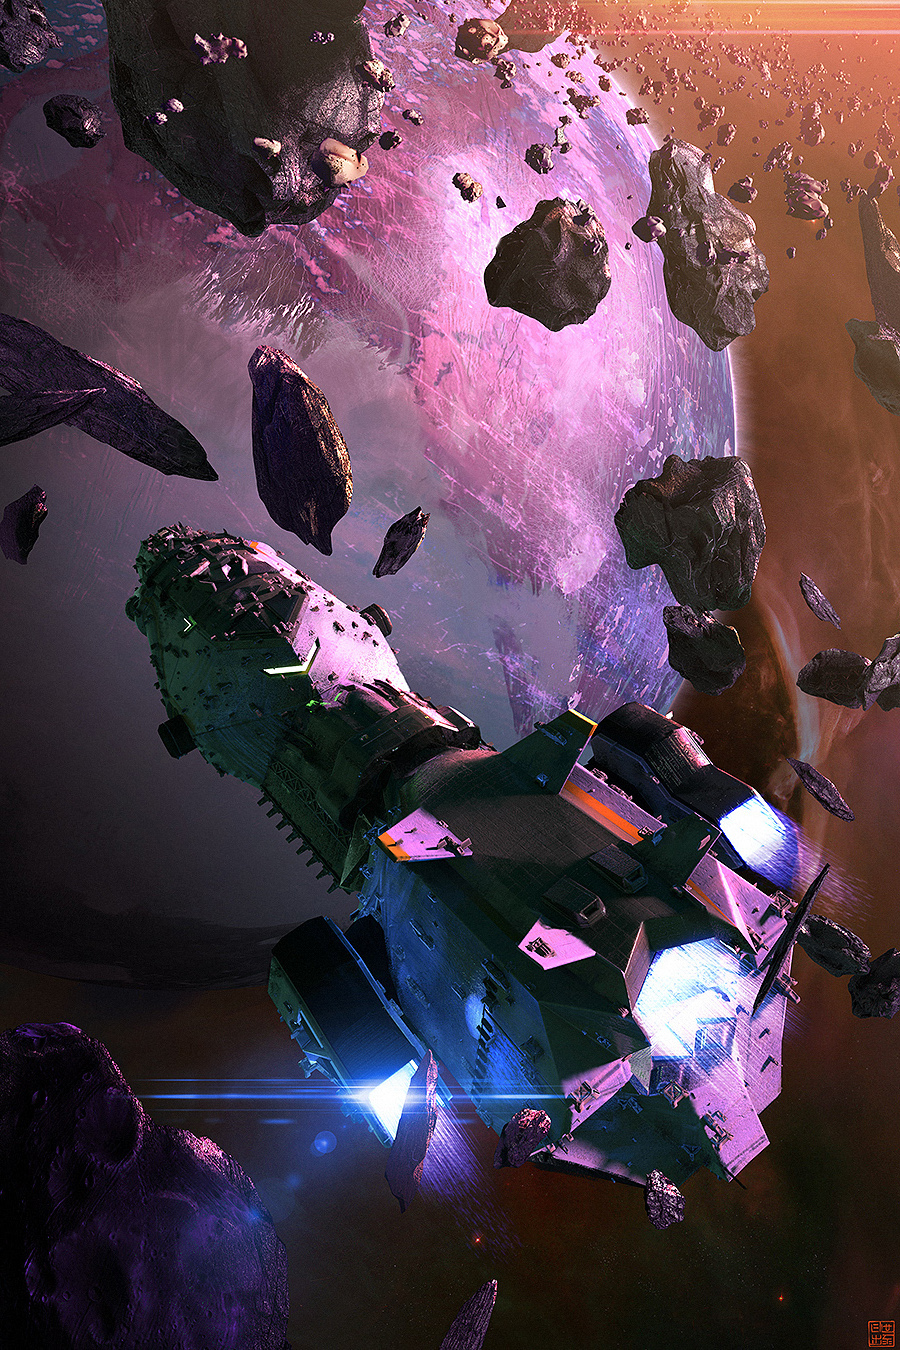
\includegraphics[width=\linewidth]{rebellion_of_stars___starship_blackbeard_by_hideyoshi-d8p607x}
  
  \subsection{The Surge}

  We call it \textbf{The Surge}, but very little is actually known about the event. Most tech-heads think it was a large shockwave of trans-dimensional energy that exploded from deep within the galactic center around about the 2800's, which simply overloaded all of our TDD tech. In a matter of seconds everyone lost their Jump Portals, TDD engines and even psionics to The Surge.

  The aftermath was terrible. Many worlds began to starve as they relied on the food imports delivered to them by the extensive FTL trade network. Other worlds slid into barbarism as they fought over now dwindling resources. All across the Black, countless worlds began their struggle due to their sudden isolation.
  
  It was even worse for the psionics. All the adult psionics suffered literal brain explosions during The Surge, leaving behind only the children (no one knows why they were spared). The children had to learn to safely harness their powers without the guidance of experienced mentors. To make it worse, they had to endure the fear and loathing of other survivors as rumours spread that The Surge was psionic handiwork.
  
  \subsection{Rebuilding the Galaxy}

  Over the last few centuries we have managed to rebuild. It isn't quite like the old days, but we are slowly piecing it back together. The one saving grace was that non-TDD tech was spared. Many planets filled the gaps left by the defunct TDD tech by adapting "outdated" tech. Some planets even refuse to advance further in fear that another Surge event could suddenly destroy all that they have built.
  
  In 3120, the Kaj tech-head Romazirash reverse engineered a safer (well, as they claimed) derivative of the TDD engine. It is called the \textbf{Intra-Dimensional Drive (IDD)}, and while it cannot travel across the whole galaxy it can travel across multiple star systems. The new IDD drive has allowed trade routes to be restored, and fledgling coalitions of planets began to carve out their small sections of galaxy to govern. 
  
  We once again turns our hungry eyes towards the edges of the Black. Warlords and petty tyrants scheme to expand their stellar domain. Reclaimers plunder the ruins of worlds that did not survive. And psionics continue to practice their skills away from the distrustful eyes of those who see the use of trans-dimensional energy as an imminent threat to their way of life.

  \textbf{Good luck out in the Black!}
  
  \textit{P.S: Remember: It's dangerous to go alone! Take friends.}
\end{multicols}

\vspace{\baselineskip}

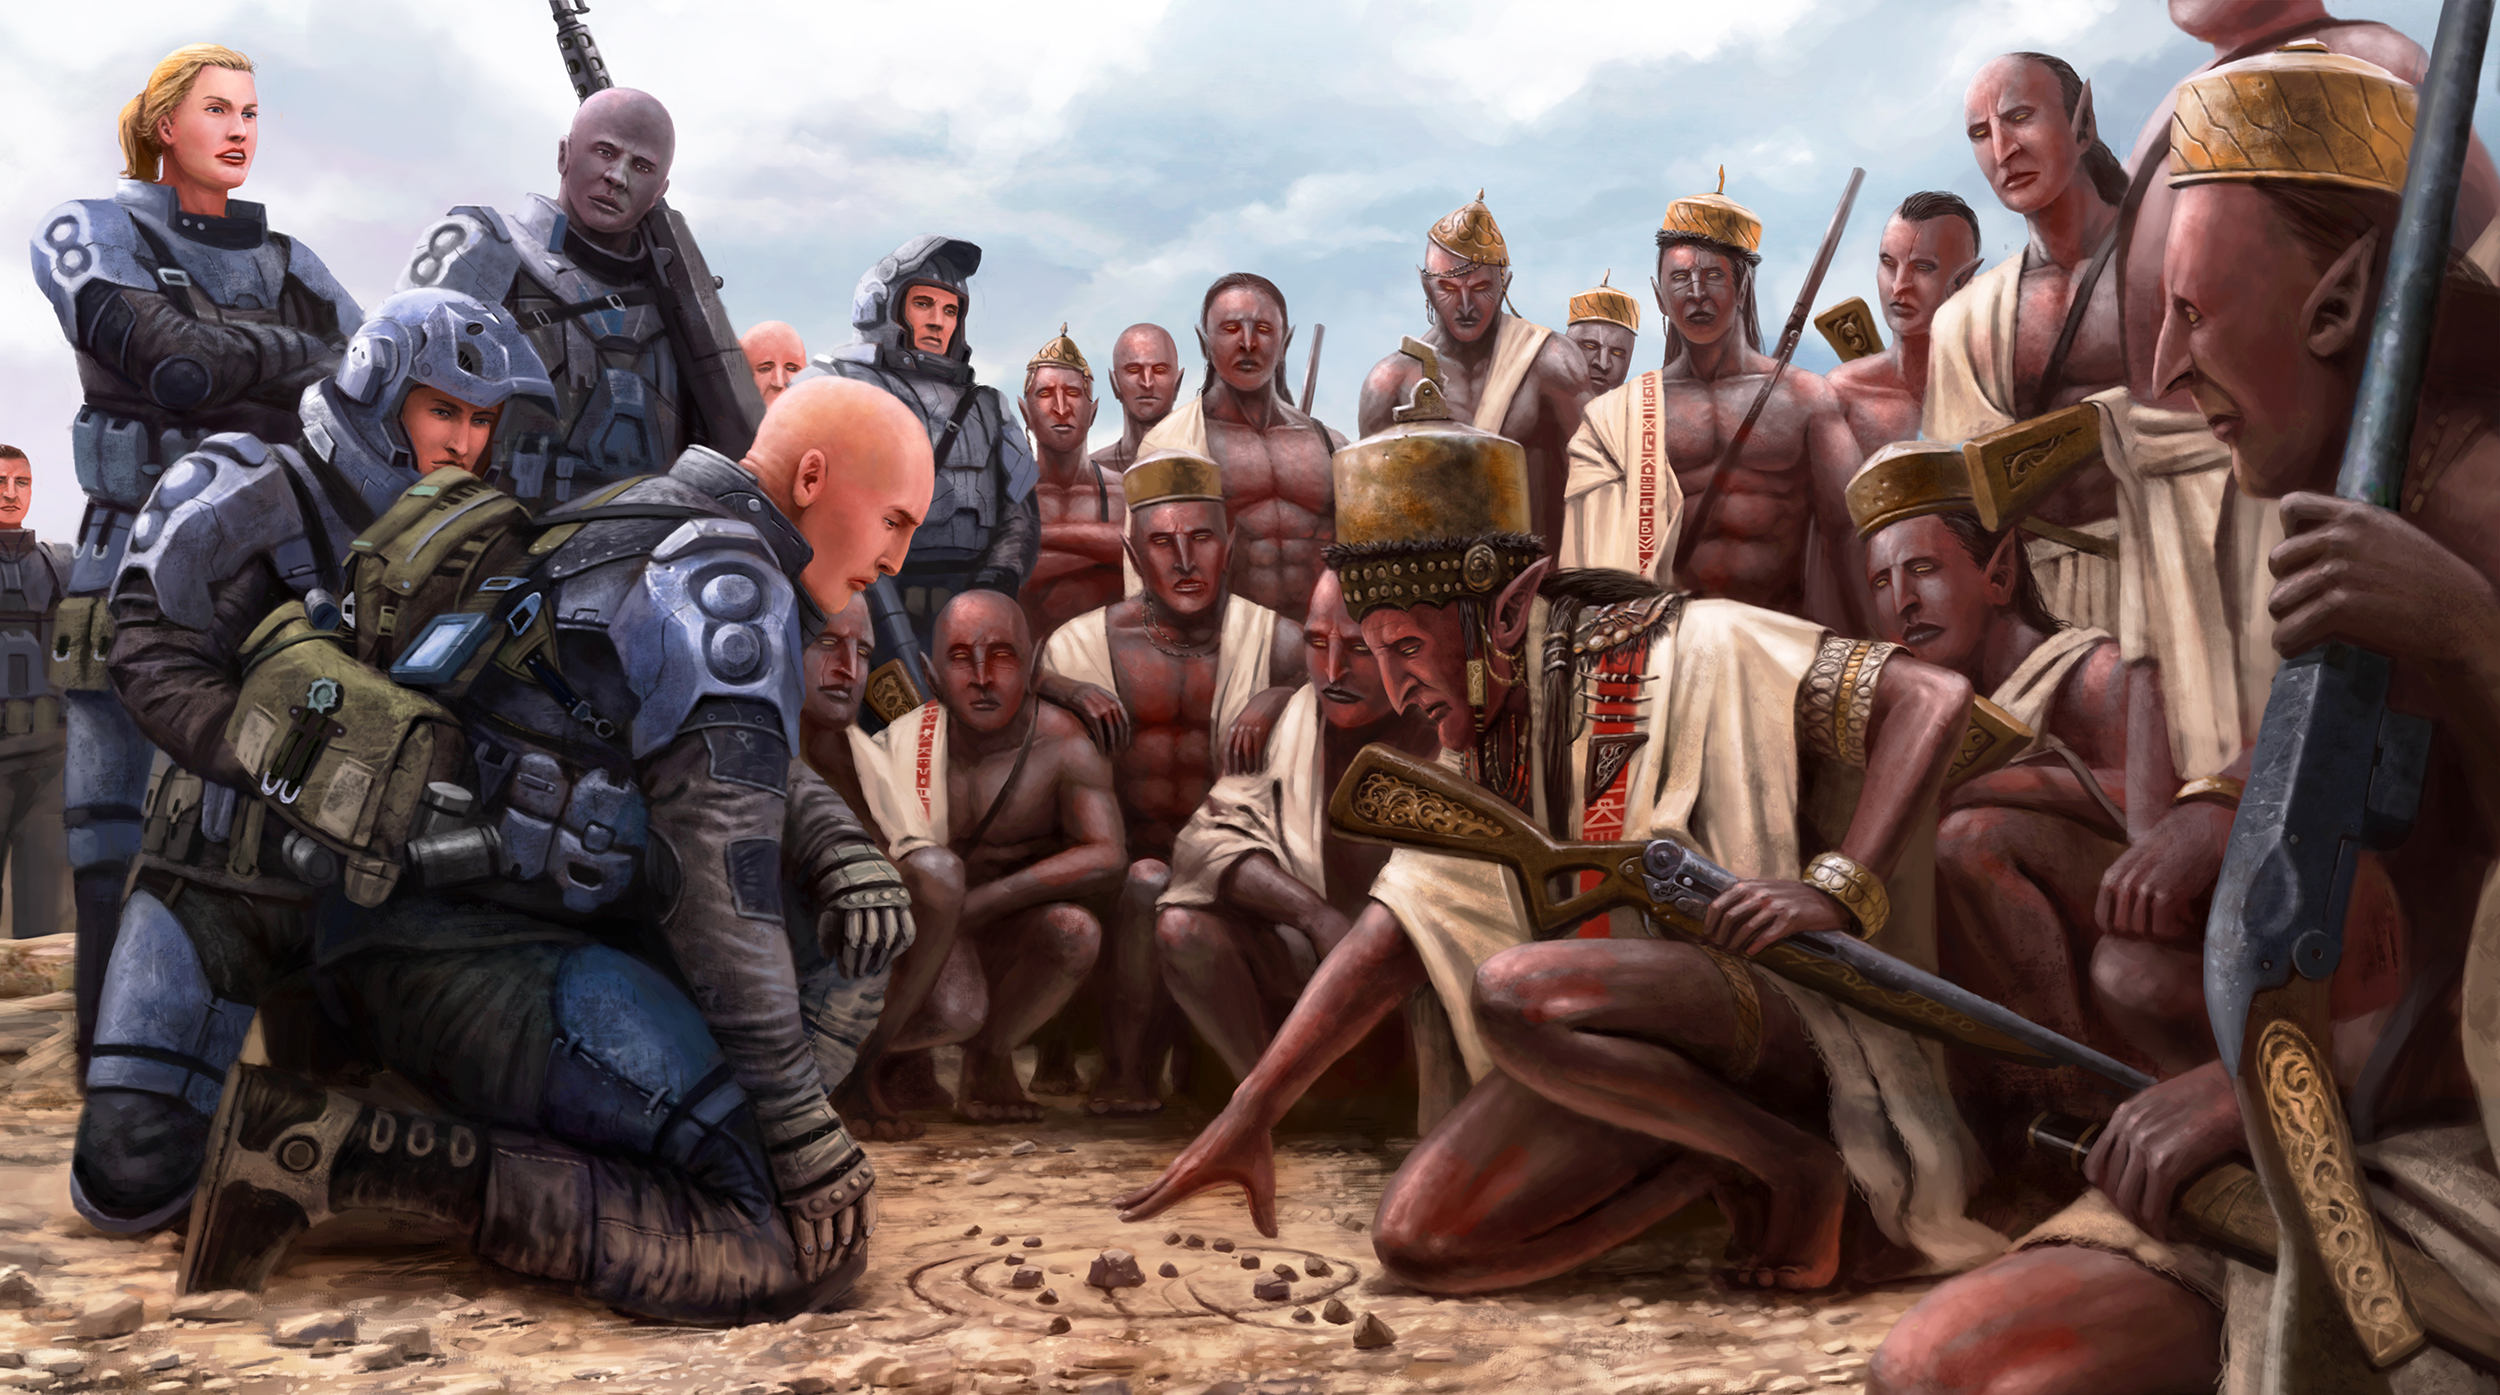
\includegraphics[width=\linewidth]{joint_operation_by_skaya3000-d6styjt}

  % Contents
  \begin{multicols}{2}
    \tableofcontents
  \end{multicols}
  % Character Creation Game Concepts & Combat rules
  % =================
% The Rules
% =================
\section{The Rules}
\begin{multicols}{2}
  \subsection{Character Creation}
\label{sec:rules-creation}

\begin{enumerate}

  \item \textbf{Species:}\\ The main species of this sector is human, although you can choose to play as a member of another alien species.
  
  \item \textbf{Attributes:}\\ You start with a d4 in each attribute and have 5 points with which to raise them. Raising an attribute by one die type costs 1 point (but you cannot raise an attribute above a d12).
    \begin{redtable}{\linewidth}{@{}L{1}@{}}
      \textbf{Strength}\\
      Raw physical power and general fitness\\
      \textbf{Agility}\\
      Nimbleness, quickness and dexterity\\
      \textbf{Smarts}\\
      Mental agility and your knowledge about the worlds that inhabit the Black\\
      \textbf{Spirit}\\
      Inner wisdom, confidence, individuality and willpower\\
      \textbf{Vigor}\\
      Endurance and a measure of how much pain and physical damage you can shake off
    \end{redtable}

  \item \textbf{Skills:}\\ You have 15 points for skills. Each die type in a skill costs 1 point up to the linked attribute. Going over the linked attribute costs 2 points per level.

  \item \textbf{Derived Traits:}
    \begin{redtable}{\linewidth}{@{}L{1}@{}}
      \textbf{Charisma}\\
      General likeability and manners, and is added to all persuasion and streetwise rolls. Calculated as: \textbf{(Spirit / 2) - 4}\\
      \textbf{Pace}\\
      How many squares of movement you can take during your turn. Calculated as: \textbf{(Strength / 2) + 2}\\
      \textbf{Parry}\\
      Target number for melee combat or against ranged weapons within melee range. Calculated as: \textbf{(Fighting / 2) + 2}\\
      \textbf{Toughness}\\
      Add armour on top of toughness. Calculated as: \textbf{(Vigor / 2) + 2}\\
    \end{redtable}

  \item \textbf{Hindrances:}\\ You can choose to gain additional character creation points by taking up to \textbf{one} Major Hindrance (2 points) and up to \textbf{two} Minor Hindrances (1 point each).
    \begin{itemize}
        \item For 2 points you can gain another attribute point or choose an \textbf{Edge}.
        \item For 1 point you can gain another skill point or increase starting funds by 100\%.
    \end{itemize}

  \item \textbf{Edges:}\\ Edges are what sets your character apart from everyone else. There are 3 main paths to choose from:
    \begin{itemize}
        \item \textbf{Standard}: Just use the normal Edge list.
        \item \textbf{Psionic}: Take the \textit{\hyperref[sec:psionics]{Psionic Background}} edge and manipulate Space-Time. (\textit{Organics only})
        \item \textbf{Cyberware}: Take the \textit{\hyperref[sec:cyberware]{Cyberware Install}} edge and enhance your abilities with tech.
    \end{itemize}

  \item \textbf{Gear:}\\ All characters start with 750 Credits to buy their equipment with.

  \item \textbf{Background Detail:}\\ Fill in any other details of your character's background. This includes selecting a homeworld, parentage, and pre-adventuring career. Every character knows the generic trade language "Basic" and their planetary dialect.
  
\end{enumerate}

\subsubsection{Advancement}

Experience points are gained by completing a game session. Each game session is worth ~1-3 points. Your character has a "\textbf{Rank}", and higher ranks allow you to access the better Edges.

\begin{redtable}{\linewidth}{@{}L{.25}@{}L{.75}@{}}
    \textbf{XP} & \textbf{Rank}\\
    0-19 & Novice\\
    20-39 & Seasoned\\
    40-59 & Veteran\\
    60-79 & Heroic\\
    80+ & Legendary
\end{redtable}

Every 5 points accumulated grants the character an Advance (or 4 Advances per Rank). One Advance allows you to do the following:

\begin{itemize}
  \item Gain a new Edge
  \item Increase one skill that is equal to or greater than its linked attribute
  \item Increase two skills that are lower than its linked attribute
  \item Buy a new skill at d4
  \item Increase one attribute (only choose this once per Rank, and no Trait can be raised above a d12)
\end{itemize}

\subsubsection{Species list}

\begin{genericsection}{Ay-Matak}
  Avian, bird-like alien species that love to travel and experience life. \textit{\hyperref[sec:specie-ay-matak]{See Species section Ay-Matak}}
\end{genericsection}
\begin{redtable}{\linewidth}{@{}L{1}@{}}
  \textbf{Flight}\\
  Can fly at their basic Pace and even "run" while flying. It cost 2 squares of Pace to gain 1 square of height\\
  \textbf{Hollow-boned}\\
  You cannot take much damage because of your hollow bones. -1 toughness\\
  \textbf{Free Edge}\\
  Start with one free Novice Edge (you must meet the requirements)
\end{redtable}
      
\begin{genericsection}{Bot}
  A standard "weak" AI hard-coded into a single chassis. \textit{\hyperref[sec:specie-bots]{See Species section Bots}}
\end{genericsection}
\begin{redtable}{\linewidth}{@{}L{1}@{}}
  \textbf{Artificial}\\
  Organics will generally prefer to deal with another organic. -2 penalty to Charisma when dealing with organics that do not know you\\
  \textbf{Construct}\\
  Add +2 to recover from being Shaken, ignore 1 level of wound penalties, do not breathe, and you are immune to poison and disease. You cannot Heal naturally, and require the Repair skill to remove wounds (use like the Healing skill)\\
  \textbf{Recharge}\\
  If you cannot access a power source at least once a day, suffer one point of Fatigue each day until Incapacitated. You must be revived with a Repair roll and a whole day of charging. If you are in this "off-line" state for more than your Vigor die in days, you effectively "die" (a new personality can be uploaded onto the chassis)\\
  \textbf{Three-Laws}\\
  Asimov's Three Laws of Robotics proved popular, but everyone wanted to tweak it. If you choose, alter your programmed "Three Laws" while keeping it's spirit. You suffer one point of fatigue if you force yourself to go against your "Three Laws"
\end{redtable}

\begin{commentbox}{\textbf{Three Laws}}
1. You may not injure an organic or allow an organic to come to harm.\\
2. You must obey orders given by organics except where such orders would conflict with the 1st Law.\\
3. You must protect your own existence as long as such protection does not conflict with the 1st or 2nd Law.
\end{commentbox}
  
\begin{genericsection}{Ghantak}
  Insectiod, beetle-like alien species that are tradition and honour-bound to serve their Queen. Contrary to popular belief, they are not part of a "hive-mind". \textit{\hyperref[sec:specie-ghantak]{See Species section Ghantak}}
\end{genericsection}
\begin{redtable}{\linewidth}{@{}L{1}@{}}
  \textbf{Carapace}\\
  You have a hard shell that can absorb most damage. +2 Armour (cannot stack with other armour; take the highest armour value)\\
  \textbf{Hidden Organs}\\
  Your vital organs are hidden away under your shell. Called shots do no extra damage against you\\
  \textbf{Restricted senses}\\
  Your unusual head restricts your field of vision. -1 to Trait rolls requiring vision\\
  \textbf{Free Edge}\\
  Start with one free Novice Edge (you must meet the requirements)\\
\end{redtable}
  
\begin{genericsection}{Ghoa}
  Violent and combative mammalian-reptilian hybrid alien species. They are all hermaphrodites, with the weaker individuals relegated to birthing duties. \textit{\hyperref[sec:specie-ghoa]{See Species section Ghoa}}
\end{genericsection}
\begin{redtable}{\linewidth}{@{}L{1}@{}}
  \textbf{Bloodthirsty}\\
  Ghoa have a reputation of being cruel to their foes and punishing captured enemies. This causes a -2 Charisma penalty when dealing with "civilized" people that do not know you (NOTE: You do not need to meet the Ghoan stereotype)\\
  \textbf{Natural Weapons}\\
  The Ghoa use their tails, claws and teeth as weapons, dealing Str+d6 damage. You are not considered an \textit{Unarmed Defender}\\
  \textbf{Reptile Blood}\\
  -4 penalty to resist negative Cold environmental effects\\
  \textbf{Stronger}\\
  Start with a d6 in Strength instead of a d4.\\
  \textbf{Free Edge}\\
  Start with one free Novice Edge (you must meet the requirements)\\
\end{redtable}
  
\begin{genericsection}{Human}
  Standard human descended from ancient Earth. Some planets have slight physical differences (such as pointed ears, greenish skin, or being short and stout) due to bio-engineering and genetic divergence. \textit{\hyperref[sec:specie-human]{See Species section Human}}
\end{genericsection}
\begin{redtable}{\linewidth}{@{}L{1}@{}}
  \textbf{Flexible}\\
  Start with a d6 in a skill of your choice\\
  \textbf{Free Edge}\\
  Start with one free Novice Edge of their choice.\\
\end{redtable}
  
\begin{genericsection}{Kaj}
  Intelligent grey-skinned humanoid alien species that generally prefer the artificial instead of the natural. \textit{\hyperref[sec:specie-kaj]{See Species section Kaj}}
\end{genericsection}
\begin{redtable}{\linewidth}{@{}L{1}@{}}
  \textbf{Artificial environments}\\
  -4 penalty to resist all negative Heat and Cold effects. If you suffer an attack based on that form, the penalty acts as a bonus to damage.\\
  \textbf{Expert}\\
  Kaj are genetically engineered to excel. Select one Skill. Anytime you make a roll with that Skill, add +2 to the result\\
  \textbf{Frail}\\
  Kaj select their genes to increase intelligence over physicality. -1 Toughness\\
  \textbf{Genetically enhanced}\\
  Kaj start with a d6 in Smarts instead of a d4.\\
  \textbf{Free Edge}\\
  Start with one free Novice Edge (you must meet the requirements)\\
\end{redtable}
  
\begin{genericsection}{Pluvma}
  Lanky, top-heavy multi-limbed alien species that generally try to stand out from the "pack". \textit{\hyperref[sec:specie-pluvma]{See Species section Pluvma}}
\end{genericsection}
\begin{redtable}{\linewidth}{@{}L{1}@{}}
  \textbf{One Eye}\\
  You have limited depth perception, so you take a -2 penalty to Trait rolls that require vision (such as Shooting)\\
  \textbf{Four Arms}\\
  You have two additional arms. This allows you to get an extra 2 non-movement actions per turn, which do not incur the multi-action penalty (they do suffer from off-hand and other penalties)\\
  \textbf{Unpredictable}\\
  The Pluvma have a reputation of being annoyingly unique, so much so that to others they seem to have a new personality everyday. -2 penalty to Charisma when dealing with non-Pluvma who do not know you (NOTE: You do not need to meet the Pluvmian stereotype)\\
\end{redtable}

\vspace{\baselineskip}
  
\begin{genericsection}{Shell}
  An advanced Artificial General Intelligence (AGI) or digitised consciousness (Ghost) that can be freely uploaded to an artificial chassis. \textit{\hyperref[sec:specie-bots]{See Species section Bots}}
\end{genericsection}

\vspace{\baselineskip}

\begin{redtable}{\linewidth}{@{}L{1}@{}}
  \textbf{Artificial}\\
  You are seen as a "traitor" or a threat to most organics. -2 penalty to Charisma when dealing with organics that do not know you\\
  \textbf{Bugs}\\
  Ghosts and AGI do not sync up perfectly with their chassis. Select one Major OR two Minor hindrances that make sense for you and the chassis. Do not gain any character creation points. This bug remains with the chassis when you transfer to another chassis\\
  \textbf{Construct}\\
  Add +2 to recover from being Shaken, ignore 1 level of wound penalties, do not breathe, and you are immune to poison and disease. You cannot Heal naturally, and require the Repair skill to remove wounds (use like the Healing skill)\\
  \textbf{Deus Ex Machina}\\
  Ghosts and AGI do not have any stats. All stats are tied to a chassis. See the following box for more information about this feature.\\
  \textbf{Disorientation}\\
  When you are first uploaded into a new chassis, you have a settling period of a few minutes (4d4 rounds OR at the GM's discretion). If you attempt to do any task during the settling period, apply a -2 penalty\\
  \textbf{Recharge}\\
  Works exactly like the "\textit{Recharge}" feature of the \textbf{Bot} class.\\
\end{redtable}

\vspace{\baselineskip}

\begin{commentbox}{\textbf{Ghost in a Shell}}
Ghosts and AGI do not have any statistics except for XP. Your XP does not grant you any advances, and is simply used to track what rank of chassis you are allowed to pilot. You do retain all of your memories, and old Ghosts and AGI may use external memory banks.\\
\\
All statistics, Edges and Hindrances are tied to a particular chassis (including the Bugs class feature). A chassis also tracks it's own separate XP (this represents your "familiarity" you have with the chassis, allowing you to "upgrade" it with up to 4 advances). A chassis cannot increase it's rank unless you pay a financial cost to improve it. You may not inhabit a chassis if you do not meet it's rank requirement (i.e. your XP rank must meet or exceed the rank of the chassis).\\
\\
You may own multiple different chassis tailored for specific jobs. You may transfer your Ghost or AGI to any chassis provided you "clear" out the old chassis; having multiple versions of "you" is illegal. 
\end{commentbox}
  
\begin{genericsection}{Uplifted}
  Genetically-altered primitive animals that have been given sentience by pre-Surge tech-heads. \textit{\hyperref[sec:specie-uplifted]{See Species section Uplifted}}
\end{genericsection}

\begin{redtable}{\linewidth}{@{}L{1}@{}}
  \textbf{Inferior}\\
  Many see the Uplifted as inferior to other species that have evolved naturally. -2 Charisma when dealing with the non-Uplifted who do not know you\\
  \textbf{Primitive Intellect}\\
  You may be uplifted, but your primitive brain is still slow. -1 to Smarts-based checks\\
  \textbf{Primal Ancestry}\\
  You have an ability due to your animal ancestor. Choose one of the following from the list.\\
  \textbf{Primal Weapons}\\
  You still have the claws, teeth, horns or other leftovers from your primitive animal state. These natural weapons do Str+d6 damage. You are not considered an \textit{Unarmed Opponent}\\
  \textbf{Free Edge}\\
  Start with one free Novice Edge (you must meet the requirements)\\
\end{redtable}

\textbf{Primal Ancestry}
\begin{itemize}
    \item \textbf{Bear:} +1 Size, and +3 Toughness (including the Size bonus). You may have difficulty fitting into gear made for normal humanoids
    \item \textbf{Bovine:} You start with a d6 in Vigor instead of a d4, and a +2 bonus to resist all negative environmental effects (heat, cold, pressure, etc)
    \item \textbf{Canine:} Low-light vision (ignore penalties for dim and dark lighting), +2 to Notice checks using smell, and choose a Skill other than Notice. Whenever you make a roll using that Skill, add a +1 bonus
    \item \textbf{Feline:} Low-light vision (ignore penalties for dim and dark lighting), and start with a d6 in Agility instead of a d4
    \item \textbf{Fish:} You cannot drown in oxygenated liquid, and have a +2 bonus when performing swimming-related checks. You also require half the amount of sleep compared to humans.
    \item \textbf{Reptile:} You regenerate faster, making a Natural Healing roll once per day instead of once per week. You also require half the amount of sleep compared to humans.
    \item \textbf{Rodent:} +4 Pace, and doubles the normal jumping distance (adds +1d6 from a successful Strength roll)
    \item \textbf{Serpent:} You can apply poison to a target using a touch-based attack (such as fangs or sting). On a success, the victim must roll Vigor or suffer a level of Fatigue. This is recovered after one hour. Multiple attacks can cause Incapacitation, but not death. You also require half the amount of sleep compared to humans.
\end{itemize} 


  % =================
% Game Concepts
% =================
\subsection{Game Concepts}
\label{sec:rules-concepts}

While all these rules will be helpful for you getting the most out of the game, there is only one process you need to remember:

\begin{enumerate}
  \item Game master will ask you to roll some dice for a skill, attribute, ability, or other trait. Find that trait on your character sheet and grab the listed dice
  \item Roll that dice AND an extra die that is called the 'Wild die'. This die is a d6
  \item Take the highest result of the two (including Aces), and apply any bonuses or penalties
  \item Give the result to the Game Master, who will tell you if you succeed or fail. The most common target to beat is a 4
\end{enumerate}

\begin{genericsection}{Aces}
If you roll the highest number on any die, you roll that die again and add it to total (and if you roll the highest again, then you keep rolling).
\end{genericsection}

\begin{genericsection}{Asphyxiation / Atmosphere}
Organics cannot survive the Black without some form of pressurized suit. On your turn, if you have not atmosphere to breathe then you must make a Vigor check every turn. For every failure you receive a Wound as you suffer decompression.
\end{genericsection}

\begin{genericsection}{Bennies}
You get 3 Bennies at start of the game (unless you have an Edge that changes that). Use them for re-rolls and other things (such as \textbf{Soaking} damage or removing \textbf{Shaken} status). You earn more bennies for doing outstanding things during the game.
\end{genericsection}

\begin{genericsection}{Cooperative rolls}
One character will declare their action, and any able and willing companions (or systems, programs and AI) can aide the player. The character will add a +1 bonus to their results for every success and raise their companions achieved on their own (maximum bonus of +4, except for Strength). Companions must have the skill to help character in their task.
\end{genericsection}

\begin{genericsection}{Disease}
There are a wide range of diseases you can experience while travelling the Black. They are broken down into different types below for easy reference. To treat a disease (unless stated otherwise), you need the required medicine. When the medicine is available, ailments vanish in 2d6 days minus half your Vigor dice (minimum one day). Incapacitation due to disease will result in death.

You can contract a disease through \textbf{Airbourne particles} (can hold breath for 2 plus Vigor die rounds, and half that if you were not prepared), \textbf{Touch} (must make a Vigor roll immediately upon being touched), and \textbf{Bloodstream Induction} (ingested, animal bite, or infected weapon. Usually caused by being Shaken during an attack).

\begin{redtable}{\linewidth}{@{}L{1}@{}}
  \textbf{Long-Term Chronic; Majorly Debilitating}\\
  You always suffer two levels of Fatigue due to coughing fits and frequent spasms. Another Fatigue level will cause Incapacitation but not death. At the start of the session you must roll a Vigor check; on a 1 or less you are going to pass away before the session ends.\\
  \textbf{Long-Term Chronic; Minorly Debilitating}\\
  Same as above but suffer one level of Fatigue instead of two.\\
  \textbf{Short-Term; Debilitating}\\
  When you contract the disease, you suffer one level of Fatigue and you are Shaken. You can recover from being Shaken, but the Fatigue level staus for 2d6 days while the sickness works itself out.\\
  \textbf{Short-Term; Lethal}\\
  Treat this as Letal Poison. If you survive, you suffer Fatigue that lasts 2d6 hours\\
\end{redtable}
\end{genericsection}

\begin{genericsection}{Dramatic Tasks}
Some actions with deadly consequences and a time limit. You must complete 5 successful rolls to resolve the task. Most tasks come with a -2 penalty to represent the intense amount of pressure the character is under.
\end{genericsection}

\begin{genericsection}{Encumberance}
Your character's load limit is 3 x their Strength die (in kilograms). Each multiple above that limit gives a -1 penalty to Agility and Strength (\textit{do not recalculate your load limit!}) and all related skills
\end{genericsection}

\begin{genericsection}{Falling}
  You suffer 1d6+1 damage per 3 meters (2 squares), up to 10d6+10. Landing in water reduces number of dice rolled by half (rounded down).
\end{genericsection}

\begin{genericsection}{Fatigue}
Fatigue represents the stresses and weaknesses your character can suffer. It acts similarly to Wounds; once you are out of Fatigue points you become incapacitated. Every level of Fatigue is a -1 penalty to all rolls. Recovering Fatigue points is highly dependant on the source; hunger requires food, cold requires warmth, and so on. The character must resolve all sources of Fatigue to recover fully.

Some fatigue sources include:
\begin{redtable}{\linewidth}{@{}L{1}@{}}
  \textbf{Cold}\\
  Make a Vigor roll every four hours while in below freezing temperatures. -1 penalty for each -5 degrees below freezing (if wearing warm clothing). Add -2 penalty if not wearing appropriate clothing. Recovers 1 Fatigue every hour in normal temperatures.\\
  \textbf{Drowning}\\
  Make an Athletics check to avoid drowning. -2 penalty if holding something up at the same time. You roll every round while in rough water. When you are out of the water, you recover 1 Fatigue level per 5 mins. Death occurs half your Vigor die in rounds after Incapacitation.\\
  \textbf{Heat}\\
  Make a Vigor roll every four hours while in extremely hot temperatures. -1 penalty for each 5 degrees above 35 degrees Celsius (if have sufficient water). Add -2 penalty if you do not have water. Recovers 1 Fatigue every hour in normal temperatures.\\
  \textbf{Hunger/Thirst}\\
  Most organics require half a kilo of food and half a litre of water every 24 hours. If you have less food than that, you must make a Vigor roll for each 12 hour period. -2 penalty if you have had little to no food. Thirst is rolled every 6 hours. If you are incapacitated by Hunger, you die 3d6 hours later.\\
  \textbf{Radiation}\\
  You must make a Vigor roll every hour spent in low radioaction, and every minute in high radiation. Radiation Fatigue fades one level every 24 hours, or half that if you are able to scrub dust and other contaminants. On Incapacitated, you suffer a Long-Term Chronic; Minorly Debilitating disease (Radiation Sickness)\\
  \textbf{Sleep}\\
  You need a minimum of 6 hours of sleep every 24 hours. You make a Vigor roll at a culmulative -2 penalty every 12 hours you do not get the required sleep. Stimulants may add a +2 bonus to the roll. Incapacitated characters fall into sleep for 2d10 hours.
\end{redtable}
\end{genericsection}

\begin{genericsection}{Fear}
To overcome your Fears you must make a Spirit roll (some monsters add a penalty to the Spirit roll). On a failure, you are Shaken and suffer a level of Fatigue for the rest of the encounter. You only need to roll a Fear check the first time you encounter the source (or experience the source again in new and uncomfortable ways).
\end{genericsection}

\begin{genericsection}{Fire}
Anytime something flammable is hit by fire, roll a d6. On a 6 that object catches on fire. Particularly vulnerable items ignite on a 4-6. Volatile targets will catch on anything but a 1. If a person catches on fire, they need to roll every round; if they succeed again, the fire catches in intensity and causes the damage listed in the table below.

Fire in confined areas create smoke, and every round you must make a Vigor roll (+2 bonus if using a wet rag to breath through). If failed, you gain a Fatigue level.

\begin{redtable}{\linewidth}{@{}L{1}@{}}
  \textbf{Burning Weapon}\\
  +2 to damage\\
  \textbf{Spot fire}\\
  1d10\\
  \textbf{Flamethrower}\\
  2d10\\
  \textbf{Lava}\\
  3d10\\
\end{redtable}
\end{genericsection}

\begin{genericsection}{Gravity}
When you are experiencing high gravity, apply a -2 penalty to all Agility-based rolls, your pace and your jump. When you are experiencing low gravity, apply a +2 bonus to all Agility-based rols, your pace and your jump. In zero-g environments, a result of 1 on a physical trait die means you lose control and tumble (-2 to all Trait rolls). To stabilise yourself while you are tumbling, you must succeed on an Agility roll as a free action (only if you have a way to stabilise yourself).
\end{genericsection}

\begin{genericsection}{Group Rolls}
To quickly roll for a group of extras (such as henchmen), simply roll one Trait die and one Wild die. Take the highest of the two as the average for the whole group.
\end{genericsection}

\begin{genericsection}{Hacking} 
Hacking is a very complex task. It will generally require the Hacker to access a physical I/O port, which is best accessed if the Bot is incapacitated. Then the Hacker needs to open the I/O port (Hacker's Repair vs Bot's Toughness), and then break the software Firewalls (Hacker's Security opposed by the Bot's Spirit). Treat Hacking as if it was a \textbf{Dramatic Task}.
\end{genericsection}

\begin{genericsection}{Healing}
The Healing skill can be used to treat any Wound suffered within the last hour and takes about 10 minutes. A success on a Healing check removes 1 Wound, and raises will removee 2. Further raises have no effect. The healer must apply the patient's Wound penalty as well as their own Wound penalty to the Healing check. Trying to heal your own wounds will effectively double your wound penalties. If you do not have suitable medical supplies you suffer another -2 penalty. After one hour, only \textbf{Natural Healing} can remove Wounds.
\end{genericsection}

\begin{genericsection}{Initiative}
Players get one card per round and act according to the deck order, which goes from the Ace to Deuce (in case of ties the suit order is Spade, Heart, Diamond, Club). If the player gets a Joker they can act whenever they want, and the Joker gives them a +2 bonus on all Tests and +2 to all Damage
\end{genericsection}

\begin{genericsection}{Movement} 
Use the following rules to determine movement.
\begin{redtable}{\linewidth}{@{}L{1}@{}}
  \textbf{Crawling}\\
  May crawl 2 squares per turn. This counts as being prone\\
  \textbf{Crouching}\\
  May move at half Pace. You may run while crouched. Ranged attacks againts you suffer a –1 penalty\\
  \textbf{Going Prone}\\
  You may fall prone at any time during your action. Getting up costs 2 units of movement\\
  \textbf{Difficult Ground}\\
  Difficult ground such as mud, steep hills, or snow, slows characters down. Count square of movement as double\\
  \textbf{Jumping}\\
  1 square horizontally from a dead stop; 2 squares with a “run and go.” A successful Strength roll grants one extra inch of distance\\
  \textbf{Running}\\
  You may run an additional 1d6 squares during your turn, but incur a -2 running penalty to all other actions\\
\end{redtable}
\end{genericsection}

\begin{genericsection}{Natural Healing}
If you have any Wounds, you must make a Vigor roll every 5 in-game days. You remove 1 Wound level (or Incapcitated status) with a success, or improve 2 steps with a Raise. A critical failure increases your Wound level by one. You subtract wound penalties from these rolls as usual. Medical attention means that someone with the Healing skill is actively checking the patient's wounds.
\begin{redtable}{\linewidth}{@{}L{.75}@{}L{.25}@{}}
  \textbf{Condition} & \textbf{Modifier}\\
  Rough travelling & -2\\
  No medical attention & -2\\
  Poor environment & -2\\
  Medical attention (pre-industrial) & -\\
  Medical attention (industrial and beyond) & +1\\
  Medical attention (robotics and beyond) & +2\\
\end{redtable}
\end{genericsection}

\begin{genericsection}{Objects and Obstacles}
Inanimate objects have a parry of 2, no additional damage from raises on attack roll (and no aces on damage). If an attack can’t do enough damage to destroy an object, it can’t be destroyed (in combat).
\begin{redtable}{\linewidth}{@{}L{.30}@{}L{.30}@{}L{.40}@{}}
  \textbf{Object} & \textbf{Toughness} & \textbf{Damage Type}\\
  Light Door & 8 & Blunt, Cutting\\
  Heavy Door & 10 & Blunt, Cutting\\
  Lock & 8 & Blunt, Piercing\\
  Handcuffs & 12 & Blunt, Piercing, Cutting\\
  Knife, Sword & 10 & Blunt, Cutting\\
  Rope & 4 & Cutting, Piercing\\
  Shield & 10 & Blunt, Cutting\\
\end{redtable}
\end{genericsection}

\begin{genericsection}{Poison}
If ingested, effects occur automatically. If Shaken or wounded by a poisoned weapon, you must make an immediate Vigor roll (some poisons may come with a modifier). To treat a poisoned character, the medic can try a healing roll minus the strength of the poison itself. You may only attempt once per incident (another character may have a try). Fatigue levels due to poison recover 1 level per 24 hours.

\begin{redtable}{\linewidth}{@{}L{1}@{}}
  \textbf{Lethal Poison}\\
  Failure results in death in 2d6 rounds. Success results in 1 wound and Exhaustion\\
  \textbf{Venomous Poison}\\
  Failure results in death in 2d6 minutes. Success results in 1 round and Exhaustion\\
  \textbf{Paralysis Poison}\\
  Failure results in paralysis for 2d6 minutes, 2d6 rounds for success\\
  \textbf{Knockout Poison}\\
  Failure results in knocked out for 2d6 hours, 2d6 minutes for success\ 
\end{redtable}
\end{genericsection}

\begin{genericsection}{Raise}
Every 4 points over the Target Number is a Raise and can give additional benefits to your roll
\end{genericsection}

\begin{genericsection}{Size}
Most humanoids (except for the Ghoa and some Uplifted) start at the default size 0. Adjustments to this value directly affects toughness (add or subtract your size from your toughness). When attacking a creature 2 or more levels smaller than you will incur a -2 attack penalty; attacking a creature 4 or more levels larger than you will gain a +2 bonus; attacking a creature 8 or more levels larger than you will gain a +4 bonus.
\begin{redtable}{\linewidth}{@{}L{.25}@{}L{.75}@{}}
  \textbf{Size} & \textbf{Example}\\
  -2 & Cat, large rat, small dog\\
  -1 & Large dog, bobcat, small humanid\\
  0 & Humanoid, Aliens\\
  +1 & Bear Uplifted\\
  +2 & Bull, Gorilla, Horse\\
  +3 & Bear\\
  +4 & Rhino, Great White Shark\\
  +5 & Small Elephant\\
  +6 & Elephant\\
  +7 & T-Rex, Orca\\
  +8 & Dragon\\
  +9 & Blue Whale\\
  +10 & Kraken, Leviathan\\
\end{redtable}
\end{genericsection}

\begin{genericsection}{Social Conflict}
Social conflicts are broken down into three rounds of conversation. Each round the characters will roleplay their arguments and make an opposed Persuasion check (+2 for good points, -2 for faux pas). Speakers gain points for each success and raise. At the end of the third round, the character with the most points wins the conflict. If knowledge is used, the character uses the lowest trait roll between their Knowledge and Persuasion.
\begin{redtable}{\linewidth}{@{}L{.25}@{}L{.75}@{}}
  \textbf{Margin} & \textbf{Result}\\
  Tie & Issue is unsettled and no action taken until new evidence can be presented\\
  1-2 & Target is not convinced but decides it is better to be safe than sorry. Provides minimal action\\
  3-4 & Target is reasonably convinced, but will require something in return for action\\
  5+ & Target is utterly convinced, and will aide in whatever way they can\\
\end{redtable}
\end{genericsection}

\begin{genericsection}{Stealth}
Guards are either inactive or active. A success on your Stealth check will mean that you avoid inactive guards; a Failure makes them active. Active guards will then make an opposed Notice check against your Stealth result; a guard's Success means that they spot you. The last square of movement around the guard will always require an opposed Stealth/Notice check. You can move 5x you Pace when outside combat per Stealth Check. In groups, use the lowest Pace. In combat, you must make one Stealth check per round. Use the following modifiers:
\begin{redtable}{\linewidth}{@{}L{.25}@{}L{.75}@{}}
  \textbf{State} & \textbf{Modifier}\\
  Crawling & +2\\
  Running & -2\\
  Dim Light & +1\\
  Darkness & +2\\
  Pitch Black & +4\\
  Light cover & +1\\
  Medium cover & +2\\
  Heavy cover & +4\\
\end{redtable}
\end{genericsection}

\begin{genericsection}{Unskilled rolls}
If you are unskilled then your roll is a d4 with a –2 penalty
\end{genericsection}

\begin{genericsection}{Wild Die}
A d6 rolled along with normal die. Player chooses highest result (but Snakeyes is a critical fail). The Wild Die can Ace and Raise like normal dice. You only have one wild die per action (even if you use multiple Trait die, such as for Autofire)
\end{genericsection}

  % =================
% COMBAT
% =================
\subsection{Combat Actions}
\label{sec:rules-combat}

During combat, every character can perform at least one movement and one non-movement action without penalty. When performing more than one non-movement action, you take a -2 penalty for each action taken in that round on ALL actions. You cannot perform the exact same action twice in the same round (for example, you need to attack with two different weapons to take the attack action twice).

Readying a weapon usually takes an entire action, but can be done faster (and will incur the multi-action penalty). If you suspect something nasty around the corner, be sure to unholster your weapon.

\begin{genericsection}{Aim}
Do not move to gain +2 to shooting next round. You may choose to instead fire at Extreme Range (up to 4x the weapon’s Long Range), at a -8 penalty (-6 with a scope). This applies to personal as well as vehicular weapons.
\end{genericsection}

\begin{genericsection}{Aftermath}
After combat finishes, you may be interested in seeing what happens to allies and enemies. Players make Vigor rolls for allies (the Game Master does the same for enemies). A success means that they are alive but \textit{Incapacitated}, and a raise means that wounds were only superficial (they may be able to move, but cannot fight or provide any other useful action).
\end{genericsection}

\begin{genericsection}{Area Effect Attacks}
All targets in the target area suffer damage. Treat cover as armour. Missed attacks cause a deviation of 1d6 for thrown weapons, 1d10 for launched weapons; x1 for Short Range, x2 for Medium Range, x3 for Long Range
\end{genericsection}

\begin{genericsection}{Autofire}
Roll a number of Shooting dice up to your weapon's RoF (Rate of Fire), but with only 1 wild die. -2 penalty to all attacks, and each dice uses up one piece of ammunition. Two or more shots always incur the -2 autofire penalty (accounting for recoil, etc)
\end{genericsection}

\begin{genericsection}{Bleeding Out}
When you are Incapacitated (\textit{\hyperref[sec:rules-concepts-incapacitated]{see Incapacitated}}) and get the Bleeding Out status, you must make a Vigor check for every round until you are \textbf{Stabilized}. This happens before any cards are dealt. If other characters make some sort of Healing roll, the character stabilizes and no more rolls are needed. The result of your Bleeding Out Vigor check is as follows:
\begin{redtable}{\linewidth}{@{}L{1}@{}}
  \textbf{Success} \\
  Roll again every round until Stabilized\\
  \textbf{Raise} \\
  You are now Stabilized and do not need to make any more rolls\\
  \textbf{Failure} \\
  Your character instantly dies from the blood loss\\
\end{redtable}
\end{genericsection}

\begin{genericsection}{Called Shots}
Allows you to target unarmoured or weak points of the enemy.
  \begin{redtable}{\linewidth}{@{}L{1}@{}}
    \textbf{Limb}\\
    -2 penalty, no extra damage but may be able to Disarm\\
    \textbf{Head}\\
    -4 penalty, +4 damage. (Target must have sensitive areas and the attacker knows where they are)\\
    \textbf{Small Target}\\
    -4 penalty. There may be additional benefits, but the default benefit is +4 damage\\
    \textbf{Tiny Target}\\
    -6 penalty. There may be additional benefits, but the default benefit is +4 damage\\
  \end{redtable}
\end{genericsection}

\begin{genericsection}{Cover}
Cover adds a penalty to all incoming attacks that target the victim. The penalty to apply depends on the type of cover, and are:
\begin{redtable}{\linewidth}{@{}L{1}@{}}
  \textbf{Light} \\
  -1 to all attacks\\
  \textbf{Medium} \\
  -2 to all attacks\\
  \textbf{Heavy} \\
  -4 to all attacks\\
\end{redtable}
\end{genericsection}

\begin{genericsection}{Darkness}
Lighting affects all actions that require lighting. Apply the following penalties:
\begin{redtable}{\linewidth}{@{}L{1}@{}}
  \textbf{Dim} \\
  -1 to all sight-based actions\\
  \textbf{Dark} \\
  -2 to sight-based actions, and targets are not visible beyond 2 squares\\
  \textbf{Pitch Black} \\
  -4 to all sight-based actions, and the target must be detected to be attacked\\
\end{redtable}
\end{genericsection}

\begin{genericsection}{Defend}
+2 bonus to Parry, and you can perform no other actions this round
\end{genericsection}

\begin{genericsection}{Disarm}
-2 penalty to your attack. On a success, the defender makes a Strength roll vs the damage or they drop their weapon
\end{genericsection}

\begin{genericsection}{Double Tap/Three Round Burst}
+1 bonus to your attack and damage rolls for a double tap using a semi-automatic weapon; +2 bonus to your attack and damage rolls for a 3RB. Each shot uses a piece of ammunition. This counts as Autofire, so the penalties still apply to the attack roll.
\end{genericsection}

\begin{genericsection}{Finishing Move}
A helpless or incapacitated victim may be dispatched as an action
\end{genericsection}

\begin{genericsection}{Ganging Up}
+1 bonus to your Fighting for each additional adjacent attacker (maximum +4)
\end{genericsection}

\begin{genericsection}{Grappling}
Make a Fighting roll to grapple, and a raise causes the victim to be Shaken. The target must roll an opposed Strength or Agility Roll to break free
\end{genericsection}

\begin{genericsection}{Improvised weapon}
    \begin{redtable}{\linewidth}{@{}L{1}@{}}
      \textbf{Small}\\
      Range 3/6/12, Damage Str+d4, RoF 1, Min Str d4, –1 attack and Parry\\
      \textbf{Medium}\\
      Range 2/4/8, Damage Str+d6, RoF 1, Min Str d6, –1 Attack and Parry\\
      \textbf{Large}\\
      Range 1/2/4, Damage Str+d8, Min Str d8, –1 attack and Parry\\
    \end{redtable}
\end{genericsection}

\begin{genericsection}{Incapacitated}
\label{sec:rules-concepts-incapacitated}
After suffering 3 Wounds you must make a Vigor check:
\begin{redtable}{\linewidth}{@{}L{1}@{}}
  \textbf{1 or Less}\\
  Your Character dies\\
  \textbf{Fail}\\
  You roll on Injury Table and effect is permanent. You are also \textbf{Bleeding Out}\\
  \textbf{Success}\\
  Roll on Injury Table. The injury is gone when healed\\
  \textbf{Raise}\\
  Roll on Injury Table. The injury is gone in 24 hours\\
\end{redtable}
\end{genericsection}

\begin{genericsection}{Injury table}
You must roll on the injury table when you are \textbf{Incapacitated}. Simply roll 2d6 and consult the table.
\begin{redtable}{\linewidth}{@{}L{1}@{}}
  \textbf{2 (Irreplaceable)}\\
  The GM determines the worst possible outcome\\
  \textbf{3-4 (Arm)}\\
  Roll left or right arm randomly; it’s unusable like the One Arm Hindrance (but can be fixed with Cyberware)\\
  \textbf{5-9 (Guts)}\\
  Roll 1d6; 1-2 reduce Agility, 3-4 reduce Vigor, 5-6 reduce Strength (minimum d4)\\
  \textbf{10 (Leg)}\\
  Gain the Lame Hindrance (or the One Leg Hindrance). This can be fixed with Cyberware\\
  \textbf{11-12 (Head)}\\
  Roll 1d6; 1-2 you have a scar and Ugly Hindrance, 3-4 you have the One Eye Hindrance (or Blind), 5-6 reduce Smarts (minimum d4).
\end{redtable}
\end{genericsection}

\begin{genericsection}{Innocent Bystanders}
If a shooting roll fails when firing into melee and the shooting die is a 1 (or a 2 with auto-fire or shotgun) a random nearby character may be hit instead
\end{genericsection}

\begin{genericsection}{Non-Lethal Combat}
Must use fists, rubber bullets or a blunt weapon (-1 to fighting to use flat side of bladed weapon). Roll damage normally. Incapacitated Extras are down for 1d6 hours. Wild Cards take wounds as normal including going to the Incapacitation table
\end{genericsection}

\begin{genericsection}{Obstacles}
If you wish to hit a target behind cover or an obstacle, the attack must have enough power to go through objects and obstacles and would hit without the cover penalty. The target can still use the obstacle as Armor.

Otherwise, your attack must beat the armour rating of an obstacle using your attack to destroy the obstacle.
    \begin{redtable}{\linewidth}{@{}L{.25}@{}L{.75}@{}}
      \textbf{Armour} & \textbf{Obstacle}\\
      +1 & Glass, leather\\
      +2 & Plate glass window, shield\\
      +3 & Modern interior wall, sheet metal, car door\\
      +4 & Oak door, thick sheet metal\\
      +6 & Cinder block wall\\
      +8 & Brick wall\\
      +10 & Stone wall, bulletproof glass\\
    \end{redtable}
\end{genericsection}

\begin{genericsection}{Prone}
Offers Medium Cover against Ranged Attacks beyond 3 squares. -2 penalty to Fighting and Parry while in close combat.
\end{genericsection}

\begin{genericsection}{Ranged Weapons in Close Combat}
Your ranged attack must beat the opponent’s Parry, and only pistol-sized or smaller weapons may be used
\end{genericsection}

\begin{genericsection}{Ranged Weapons modifiers}
    \begin{redtable}{\linewidth}{@{}L{.25}@{}L{.75}@{}}
      \textbf{Range} & \textbf{Modifier}\\
      Close & 0\\
      Medium & -2\\
      Long & -4\\
    \end{redtable}
\end{genericsection}

\begin{genericsection}{Rapid Attack}
Make up to 3 Fighting attacks at a –4 penalty; or fire up to 6 shots from a semi-automatic weapon or revolver at a –4 penalty to each die (this penalty already includes the Autofire penalty); this will give you a -2 Parry until your next turn
\end{genericsection}

\begin{genericsection}{Reloading}
Reloading is always an action. Running and reloading requires an Agility roll with a -2 running penalty
\end{genericsection}

\begin{genericsection}{Shaken}
Characters are Shaken when they first take damage. On their next turn, make an immediate Spirit roll (\textit{or you may use Bennies to remove Shaken status without a roll})
\begin{redtable}{\linewidth}{@{}L{1}@{}}
  \textbf{Success}\\
  Not Shaken but may only do Free Actions\\
  \textbf{Raise}\\
  Not Shaken and may act normally\\
  \textbf{Fail}\\
  Still Shaken, may only do Free Actions\\
\end{redtable}
\end{genericsection}

\begin{genericsection}{Soaking}
When you take damage, spend a Benny to make a Soak Roll (a Vigor check) to regain 1 Wound. Raises take away +1 Wound per Raise. If all the wounds are Soaked it removes any Shaken condition
\end{genericsection}

\begin{genericsection}{Suppressing Fire}
Make an attack roll with normal Autofire and range penalties. On a success, targets under a Medium Burst must make a Spirit roll or become Shaken (or are hit on 1). This will uses 5x your weapon's RoF in Ammo
\end{genericsection}

\begin{genericsection}{Test of Wills}
Intimidation (vs Spirit) and Taunt (vs Smarts) against a target. On a success you gain a +2 bonus to your next action against the Target (and Target is Shaken on a raise)
\end{genericsection}

\begin{genericsection}{The Drop}
When you catch the opponent off-guard, you are considered to be On Hold (Initiative) and add +4 bonus to attack and damage rolls
\end{genericsection}

\begin{genericsection}{Touch Attack}
When an ability or Edge asks you to make a Touch Attack, add a +2 bonus to the Fighting roll
\end{genericsection}

\begin{genericsection}{Trick}
Opposed Agility or Smarts (depending on the type). On a success Target has -2 penalty to parry, and is Shaken and distracted on raise
\end{genericsection}

\begin{genericsection}{Two Weapons}
Using two or more weapons imposes the multi-action penalty of -2 to your attacks, and a additional -2 penalty to your off-hand weapon (unless you are Ambidextrous)
\end{genericsection}

\begin{genericsection}{Unarmed Defender}
Armed attacker gains +2 on their Fighting roll
\end{genericsection}

\begin{genericsection}{Unstable Platform}
-2 penalty to Shooting from a moving vehicle or animal
\end{genericsection}

\begin{genericsection}{Wild Attack}
You choose to go berserk. +2 bonus to Fighting, +2 bonus to damage, but -2 penalty to Parry until next action
\end{genericsection}

\begin{genericsection}{Withdrawing From Melee}
Adjacent foes get 1 free attack at retreating hero's
\end{genericsection}

\begin{genericsection}{Wounded}
Player characters have 3 Wounds, while NPCs/Extras only have 1 Wound. When they run out of Wounds they are Incapacitated. To get a Wound, you must take damage when you are Shaken. Each wound is a –1 penalty to Pace and all Trait Tests (including Healing rolls). \textit{You may use Bennies to make a Soak Roll, or to remove the Shaken status}
\end{genericsection}

\end{multicols}
\newpage
% =================
% Skills
% =================
\subsection{Skills}

\begin{rpgtable}{itemtablepink}{white}{ @{} p{.20\linewidth} @{} p{.10\linewidth} @{} p{.70\linewidth} @{} }
    \textbf{Skill} & \textbf{Attribute} & \textbf{Examples}\\
    Astrogation & Smarts & Navigating safe FTL travel through the Black\\
    Astronautics & Smarts & Designing and building a spacecraft (only need the Repair skill to fix spacecraft)\\
    Athletics & Strength & Swimming, climbing, running, pushing, pulling, and weight-lifting\\
    Battle & Smarts & Military strategy and tactics. Useful for running large combat operations\\
    Bureaucracy & Smarts & Intimate knowledge about how society and governments operate. Includes Law, Economy and Administration\\
    Business & Smarts & Intimate knowledge about how to run a business or corporation. Includes Trading and wealth creation\\
    Computers & Smarts & Computers, Cyberware, Electrical, Electronics, Robotics and other computer theory\\
    Driving & Agility & Control any type of ground or water vehicle\\
    Fighting & Agility & Covers all hand-to-hand (melee) attacks and thrown weapons (from grenades to spears)\\
    Healing & Smarts & First Aid and treating existing injuries (Success and raise eliminates 1 wound). Must subtract patients wounds in addition to own wounds when making a Healing roll\\
    Insight & Smarts & Understand the motives or thoughts of someone, and scrutinizing people to see if they are lying\\
    Investigation & Smarts & Gather information from books, computers, and general research (as opposed to the Streetwise skill).\\
    Intimidation & Spirit & Frightening enemies and making threats\\
    Knowledge (Specialties) & Smarts & Other theoretical area of expertise outside of "common knowledge" (such as History, Archaeology, Philosophy, Chemistry, Mathematics, Biology, Botany, Ecology, Physics, Geology, Hydrology, and Meteorology)\\
    Language (Specialties) & Smarts & One Non-native language other than Basic, such as a planetary dialect or alien language. (\textit{d4 = common phrases, d6 = halting conversation, d8 = fluent, d10 = mimic dialects, d12 = recite important literary works})\\
    Medicine & Smarts & Latest medical theories on surgery, disease diagnosis, and epidemic containment\\
    Notice & Smarts & General alertness, searching for items, and detecting ambushes\\
    Operations & Smarts & Operate sensors, communications and other spacecraft systems\\
    Persuasion & Spirit & Convincing others. Five personality states are Hostile, Uncooperative, Neutral, Friendly and Helpful\\
    Piloting & Agility & Control any type of air or space craft\\
    Psionics & Spirit & Required for psionic characters to use their powers. For non-psionic characters, this skill represents their understanding of how psionics work\\
    Repair & Smarts & Fix gadgets, vehicles, weapons and other machines. Apply -2 penalty if you do no have the required tools\\
    Security  & Smarts & Hacking, disarming traps, bypassing alarms, cryptography, and opening locks. Use this skill to protect against intruders\\
    Shooting & Agility & Covers all ranged attacks.\\
    Stealth & Agility & Hide and move quietly, as well as palm objects and pick pockets\\
    Streetwise & Smarts & Gather information from people and the locals (as opposed to the Investigation skill). Includes tracking people in urban environments\\
    Survival & Smarts & Find food, water and shelter in hostile environments. Includes tracking people in natural environments\\
    Taunt & Smarts & Test of will attack against an opponent\\
\end{rpgtable}


  % Species
  % =================
% Species
% =================
\section{Species}
  
\begin{multicols}{2}
  \subsection{Ay-Matak}
\label{sec:specie-ay-matak}

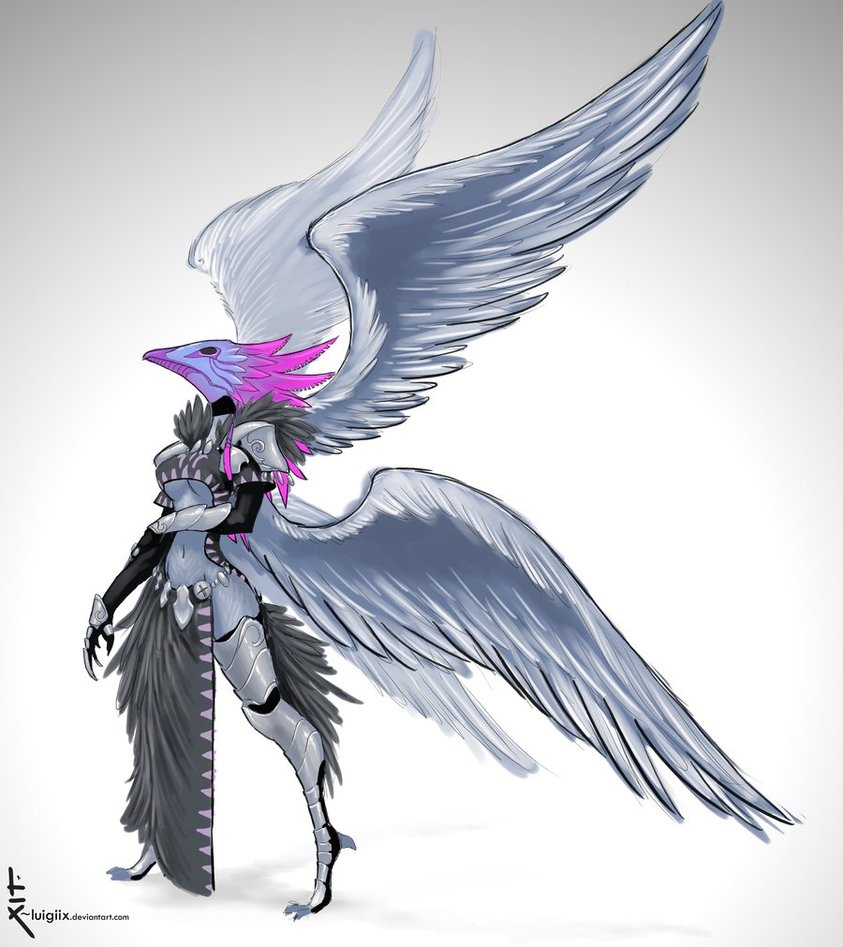
\includegraphics[width=\linewidth]{bird_race_f_concept_by_luigiix-d52w3as}

\begin{redtable}{\linewidth}{@{}L{.35}@{}L{.65}@{}}
  \textbf{Singular} & Matak\\
  \textbf{Plural} & Ay-Matak\\
  \textbf{Adjective} & Matakian\\
  \textbf{Height} & 135-170cm\\
  \textbf{Weight} & 45-65kg\\
  \textbf{Gender Ratio} & 40\% Male / 60\% Female\\
  \textbf{Reproduction} & Oviparity (Eggs)\\
  \textbf{Maturity} & 15 years\\
  \textbf{Lifespan} & 75 years\\
  \textbf{Language} & Kitabian\\
  \textbf{Diet} & Omnivore\\
  \textbf{Homeworld} & Kitaba (Lost)\\
  \textbf{\hyperref[sec:sector-atb]{ATB preference}} & \hyperref[sec:sector-atb]{B-W-H}
\end{redtable}

The Ay-Matak are an avian-like alien species from the world of Kitaba. They were one of the founding races of a Federation that spanned the galaxy before the Surge, renowned for being itinerant wanderers and creative artists. Matakian society focused on culture over conquest, but did not shy away from confrontation when it became unavoidable.

To create a Matak character, please refer to the \textit{\hyperref[sec:rules-creation]{Character creation section}}

\begin{genericsection}{Background}
Kitaba was rumoured to have a tall, dense forest that covered the entire planet and boasted a rich and diverse ecosystem. An overabundance of resources meant that the Ay-Matak had little need to compete with each other. Matakian society evolved to compete culturally rather than physically, leading to a rich and complex history of artistic endeavour. Arts that use an abundance of colour or visual stimuli are especially valued by the Ay-Matak.\\

Matakian governance also revolved around artistic endeavour, with their leaders usually a person of great cultural importance. Democracy was usually limited to recognizing the cultural importance of an individual. Once a Matak achieved that recognition they were able to join the select few who governed and directed Matakian society.
\end{genericsection}

\begin{genericsection}{Physiology}
Ay-Matak are typically shorter and lighter than other bipedal humanoids. They have two pairs of wings that enable them to fly, but they have a pair of functional legs that they use to walk on the ground. Their beak is solid and sharp along the sides, but the tip is made out of softer material so that is flexible enough to produce a variety of sounds.\\

The feathers of a male Matak is always more colourful than the female. Females are usually only limited to whites, greys and blacks.
\end{genericsection}

\begin{genericsection}{Male Names}
Andomion, Antakon, Artenaeon, Demoleo, Dralop, Entardion, Eraton, Eratro, Heliodo, Ikotu, Kalipon, Koron, Lokinu, Melaleimon, Myrodon, Panolio, Taramio, Teladon, Tridru, Tyrorion
\end{genericsection}

\begin{genericsection}{Female Names}
Agara, Alanie, Aldorria, Anakia, Atria, Bellaleta, Belliana, Hallia, Iripira, Karellia, Katia, Kynie, Laleta, Nerian, Nolanta, Obemona, Peneleta, Talitian, Tiakia, Utriema
\end{genericsection}

\begin{genericsection}{Secondary Names}
Ay-Matak do not take family names, but instead earn cultural "\textit{titles}" for their last well-known greatest achievement. For example, \textit{Andomion, painter of 'Matak Lost'}. Those without a great achievement usually go by their occupation, birthplace, spacecraft name, or include the name of their mother ("\textit{hatchling of Anakia}").
\end{genericsection}

  \columnbreak
  % =================
% Bots
% =================
\subsection{Bot/Shell}
\label{sec:specie-bots}

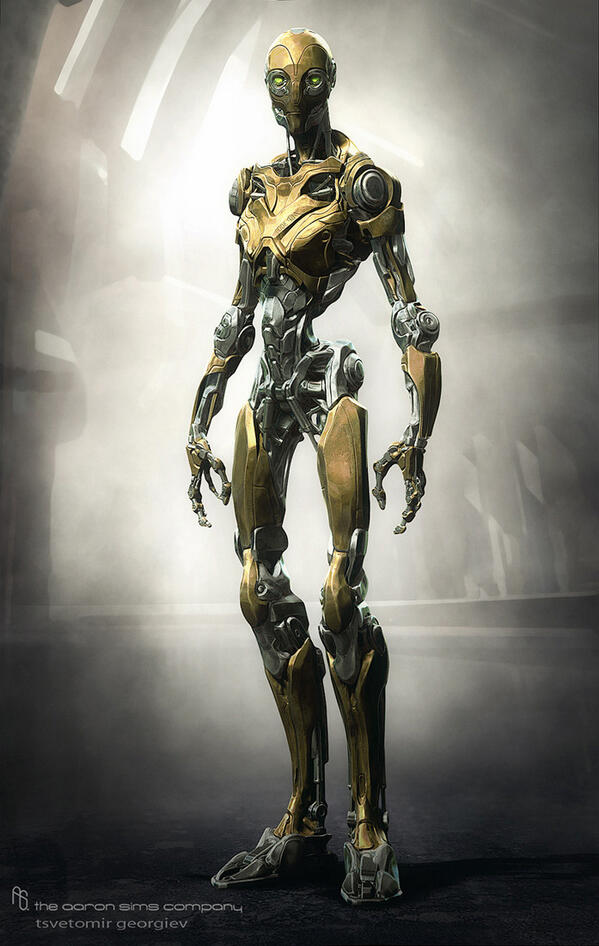
\includegraphics[width=\linewidth]{BEzZuPdCEAAgcr8}

Bots, Ghosts, Shells. These are the names given to the digital constructs that work and live beside organics. Many organics do not trust these artificial "beings" because they fear that the robots will take their jobs (and even murder them). Because of advances in material technology (especially in the field of plastics and light metals), you are not significantly heavier than most organics. Heavy bots will take an excessive amount of energy to move, so lighter Bots and Shells are the norm across the Black.

To create a Bot, Ghost or AGI character, please refer to the \textit{\hyperref[sec:rules-creation]{Character creation section}}\\

\begin{genericsection}{"Weak" AI \& Bots}
Most Bots are limited to a singular purpose by their programming, and are designed to operate in a single chassis optimized for their task. They do have advanced Neural Network pathways, fuzzy systems and deep memory to help them overcome obstacles and solve problems related to their duties. A few advanced models even have a limited sense of self, blurring the lines between normal Bots and an AGI.\\

Robots limited in this way are known as "weak AI".
\end{genericsection}

\begin{genericsection}{AGI, or true AI}
An Artificial General Intelligence (AGI) is loosely defined as a digital entity that has fully developed the ability to understand that other people, creatures and objects in the world may have thoughts, emotions and motives that can affect it's own behavior. It also has full self-awareness, and can at times seem almost indistinguishable from normal organics. Scholars debate whether these digital entities can actually have "feelings" or other properties that are associated with organic beings.
\end{genericsection}

\begin{genericsection}{Ghosts and their Shells}
There are some organic individuals who have made the transition to become fully digital. These individuals, known as Ghosts, have chosen to digitize their consciousness and upload themselves into artificial bodies known as Shells. Many in society believe that these digitized consciousnesses have lost their basic "humanity", and are indistinguishable from an AGI.
\end{genericsection}

\begin{genericsection}{The Cortical Stack}
The Cortical Stack is the most important piece of hardware for any digital entity. The Stack is where their "consciousness" is stored. The entity can usually retain their memories and personality when their Stack is transferred to a new chassis (although "weak" AI cannot operate a chassis significantly different from their own due to their limited programming).

It also should be noted that it is \textbf{highly illegal} to run multiple copies of yourself throughout most civilized planets. This is because generally the digital clones try to "murder" each other so that they can become the official version of the consciousness (among other fears).
\end{genericsection}

\begin{genericsection}{Becoming the System}
A Ghost or AGI can sometimes inhabit other digital systems such as servers and computers. Keep in mind the following:
\end{genericsection}

\begin{itemize}
  \item \textbf{Hardware}: Not all computer systems have the hardware needed to hold and operate a Ghost or AGI. In these cases it is better to hack the system instead\\
  \item \textbf{Limited Sensors}: Most systems do not even bother with audio/visual input, relying on a user to type in commands through a terminal or keyboard\\
  \item \textbf{Illegal}: Unless expressly given permission to do so, and the existing system does not already have an AI.\\
\end{itemize}

  \columnbreak
  \subsection{Ghantak}
\label{sec:specie-ghantak}

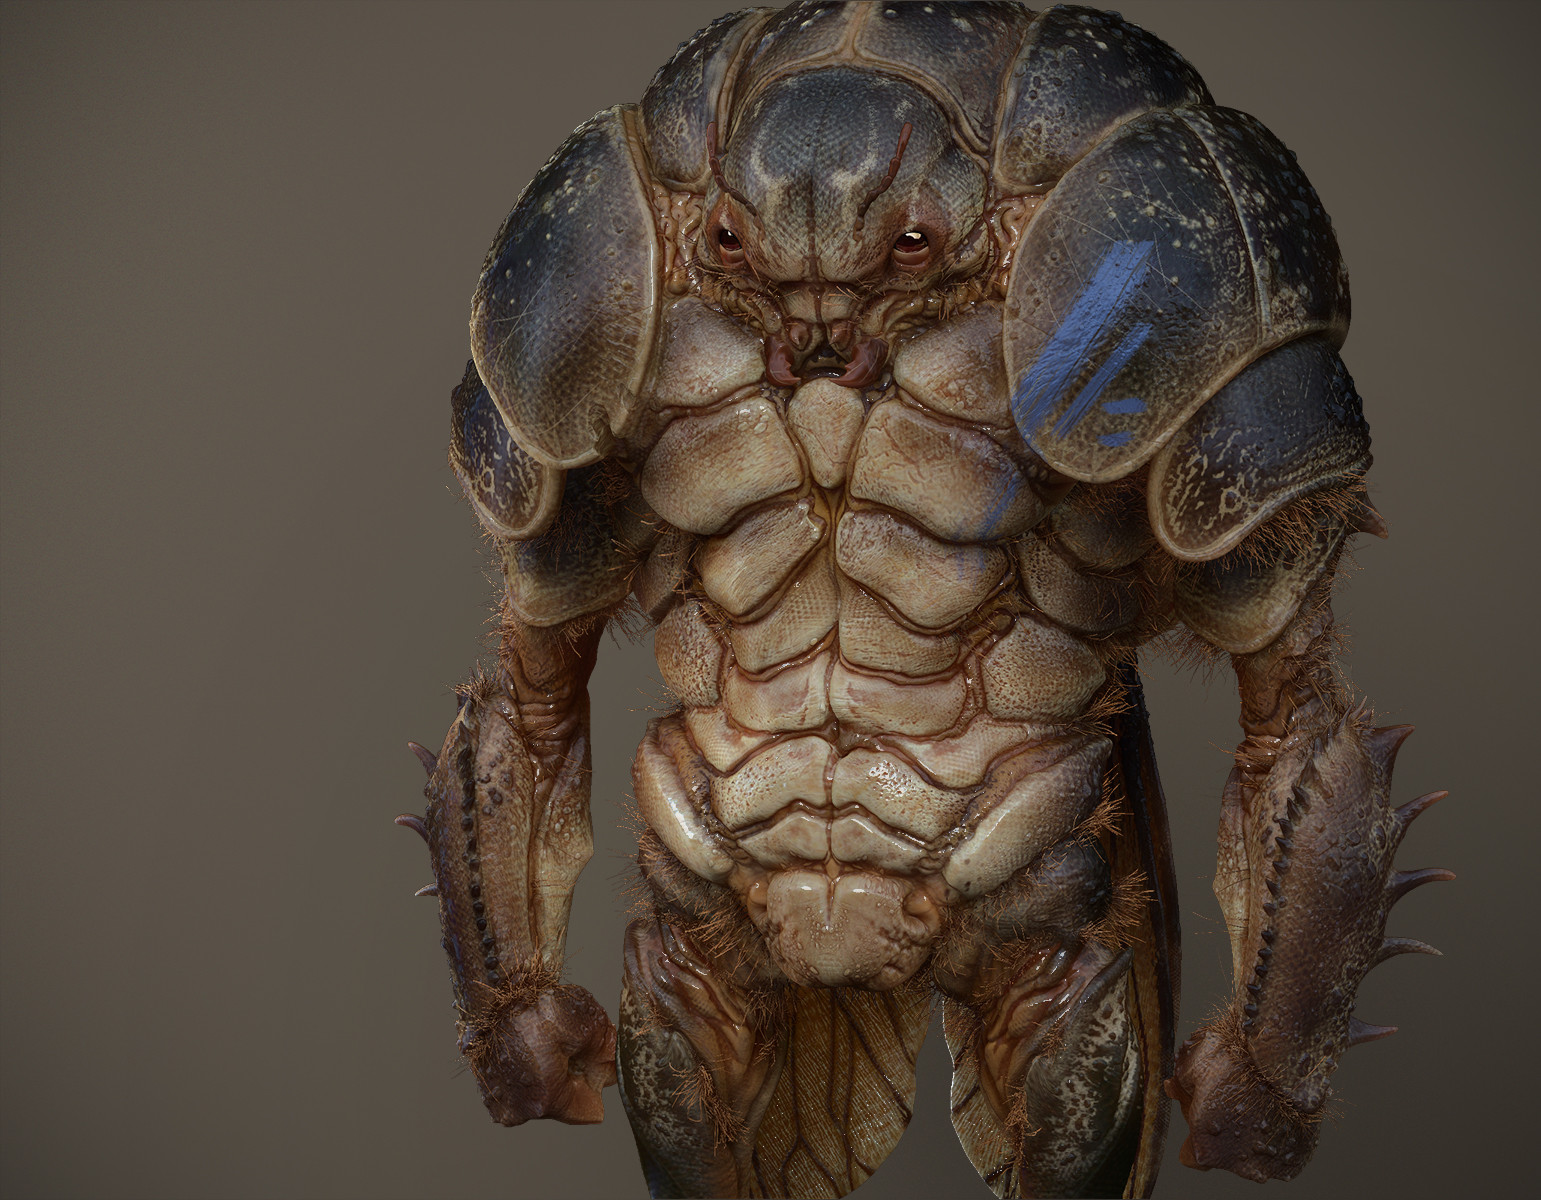
\includegraphics[width=\linewidth]{bruno-camara-beetle-brunocamara}

\begin{redtable}{\linewidth}{@{}L{.35}@{}L{.65}@{}}
  \textbf{Singular} & Ghan\\
  \textbf{Plural} & Ghantak\\
  \textbf{Adjective} & Ghantakian\\
  \textbf{Height} & 135-170cm\\
  \textbf{Weight} & 55-90kg\\
  \textbf{Gender Ratio} & 90\% Genderless / 9\% Male / 1\% Female\\
  \textbf{Reproduction} & Ovuliparity (External egg fertilization egg)\\
  \textbf{Maturity} & 5 years\\
  \textbf{Lifespan} & 60 years\\
  \textbf{Language} & Ghan\\
  \textbf{Diet} & Herbivore\\
  \textbf{Homeworld} & Ghan\\
  \textbf{\hyperref[sec:sector-atb]{ATB preference}} & \hyperref[sec:sector-atb]{B-T-C}
\end{redtable}

The Ghantak are an alien species evolved from the beetle-like insects native to their homeworld of Ghan. They are shorter than humans but weigh about the same, have an armoured carapace that covers their whole body, and their head is between the shoulders where the human chest would be. The odd placement for a Ghan head means that they must turn their whole body to look around.

Although each individual has their own free will, the Ghantak as a species have an innate tendency to organise themselves into highly-structured hierarchies. Most Ghan highly value honour and tradition, with personal sacrifice to uphold Ghantak values earning an individual glory and esteem. The race generally favours traditional solutions to problems, and individuals are uncomfortable when forced to exercise their own judgment.

While there used to be multiple independent hierarchies (each with their own Queen), the entire modern Ghantak society is now ruled by a singular Empress. The Empress is chosen from the Queens of the remaining hierarchies and she rules until her death.

To create a Ghan character, please refer to the \textit{\hyperref[sec:rules-creation]{Character creation section}}

\textbf{Ghantakian Names:}

Akiesuh, Bazoh, Bolbih, Choxu, Etix, Farqae, Gaknu, Graux, Greex, Havzal, Leksur, Mamobah, Mezuat, Semunu, Sydesih, Thonox, Vexoh, Zimla, Zouh, Ziuzoch

\textbf{Secondary Names:}

Ghantak do not take secondary names. Ghantakian first names are generally unique enough for a specific region. If pressed, the Ghantak will choose the next available incremental number for the region and their name.

\textbf{Males and Females:}

Females are especially reverred in Ghantakian culture, and are fanatically protected by all Ghantakians. They are rarely seen by non-Ghantakians, but can be differentiated by their large birthing pouch located just above their rectum. Males are also important to Ghantakian society, and usually are kept close to females to help breed the new generation. Males are allowed to travel the Black, and are almost indistinguishable from the genderless Ghantak (their genitalia is usually sheathed and protected by their carapace).

  \columnbreak
  \subsection{Ghoa}
\label{sec:specie-ghoa}

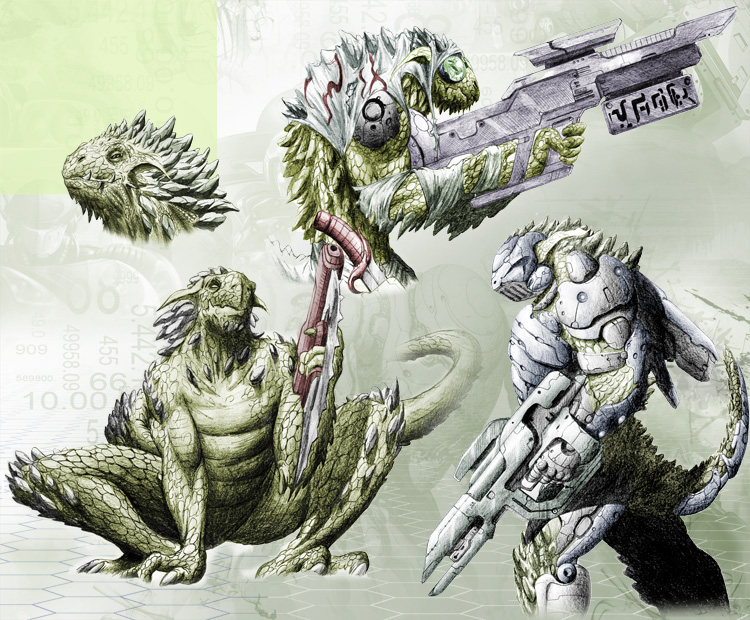
\includegraphics[width=\linewidth]{alien_reptile_concept_by_xjager513-d3ba4g7.jpg}

\begin{redtable}{\linewidth}{@{}L{.35}@{}L{.65}@{}}
  \textbf{Singular} & Ghoa\\
  \textbf{Plural} & Ghoa\\
  \textbf{Height} & 170-220cm\\
  \textbf{Weight} & 70-130kg\\
  \textbf{Gender Ratio} & 100\% Hermaphrodite\\
  \textbf{Reproduction} & Viviparity (Live birth)\\
  \textbf{Maturity} & 5 years\\
  \textbf{Diet} & Omnivore (meat preference)\\
  \textbf{Homeworld} & (\textit{Unknown})\\
\end{redtable}

The Ghoa are an alien species evolved from an unusual mammal-reptile hybrid native to their homeworld. Their homeworld has been lost to time as the Ghoa place little value on sentimental ties and recorded histories. They are larger and heavier than humans, with sharp ridged scales covering their back. They also have sharp claws and teeth, and have been known to use their tail as a weapon.

The Ghoa are typically tribal, putting their tribe ahead of all other social groups (including the species as a whole). Their chief mode of expression is anger, and the Ghoa are prone to acts of wanton violence. Disputes are traditionally resolved through force, but rarely to the death. Some Ghoa actively embrace the honour and glory of death in battle, and actively seek out combat as mercenaries and pirates.

All Ghoa are hermaphrodites, meaning they have both male and female genitals. Pregnancy is an undesirable period for any Ghoa (as it makes you weaker and more vulnerable during combat), so "females" are usually the Ghoa who are incapable of fighting and have been forced to be subservient to other Ghoa (usually the whole tribe). "Females", or "Breeders", are constantly pregnant in order to produce many warriors for the tribe.

To create a Ghoan character, please refer to the \textit{\hyperref[sec:rules-creation]{Character creation section}}

\textbf{Ghoan Names:}

Bonmok, Chardo, Drothax, Druthak, Dunmom, Garuga, Grintaz, Krudrar, Lakuq, Lugrub, Mugarod, Okrih, Pok, Rok, Roslarb, Sabub, Shak, Shopurd, Trougha, Zugorim

\textbf{Secondary Names:}

Ghoa use their tribe as a secondary name. Tribal names are usually descriptive, grandiose, or violent. Tribes are extremely fluid, as new ones are created all the time and do not need to be limited to the Ghoa only (some Ghoa see their teammates as part of their "tribe" and will take on the spacecraft name).

  \columnbreak
  \subsection{Kaj}
\label{sec:specie-kaj}

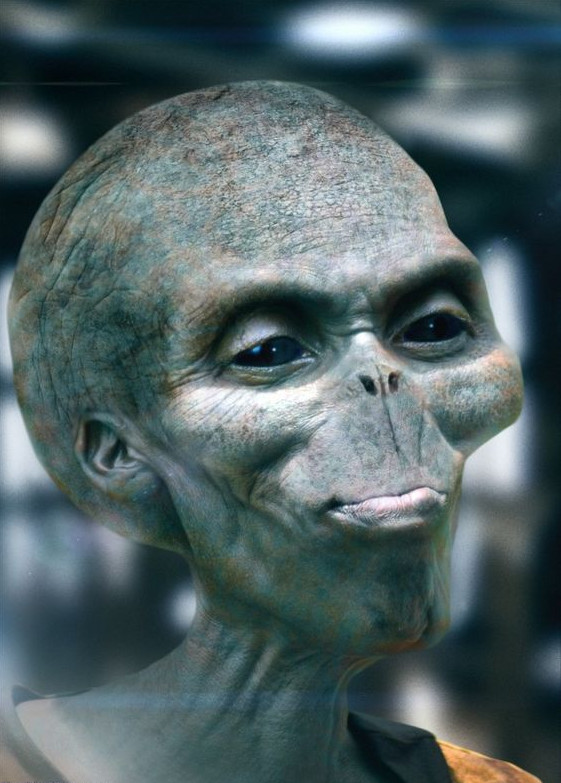
\includegraphics[width=\linewidth]{7e9dc5cf139ae3df9568cfd9921ba9b5}

\begin{redtable}{\linewidth}{@{}L{.35}@{}L{.65}@{}}
  \textbf{Singular} & Kaj\\
  \textbf{Plural} & Kaj\\
  \textbf{Height} & 150cm\\
  \textbf{Weight} & 55kg\\
  \textbf{Gender Ratio} & 100\% Clones\\
  \textbf{Reproduction} & Cloning\\
  \textbf{Maturity} & -\\
  \textbf{Diet} & Omnivore\\
  \textbf{Homeworld} & -\\
\end{redtable}

The Kaj are a highly intelligent species that have long ago decided to abandon the natural world and fully embrace artificial environments. The Kaj even went so far as to reject sexual reproduction and replace it with genetic engineering and cloning. While cloning has allowed the Kaj to artificially raise the intellectual quotient of their species, it has also left them susceptible to genetic diseases and viruses. This weakness to disease means that most Kaj keep a wary distance from outsiders, and zealously practice the highest hygiene standards and procedures.

They have also rejected their natural home planet, erasing the co-ordinates so that no Kaj could ever return. The Kaj generally choose to live in artificial spaces such as spacecrafts, space stations, and bubble colonies. To other species it seems that the Kaj have a driving desire to control their environment, but to most Kaj it is simply that they know better than the random processes that create the natural world.

Their is a schism of thought within Kaj society about whether or not the species as a whole should embrace the artificial completely and digitize their consciousness. Some see Digitization as the logical continuation of the Kaj improving upon the natural, while many fear that Digitization is a false path and would lead to the eradication of the Kaj as a species (and culture) from the galaxy. There is a whole spectrum of opinion regarding Digitization, and this opinion usually manifests itself through how much cyberware the Kaj has. A minority of Kaj even reject the cultural acceptance of the artificial, and aim to help the Kaj rediscover the natural world.

To create a Kaj character, please refer to the \textit{\hyperref[sec:rules-creation]{Character creation section}}

\textbf{Kaj Names:}

Abupikal, Brohekano, Debimaum, Fawaroum, Frukasoiro, Gatuxund, Hanepim, Ibaxi, Nothano, Osoluga, Qitandok, Romazirash, Rumduvish, Schapruga, Strikzan, Tirwein, Xintegi, Zefinag, Zosdash, Zulaum

\textbf{Secondary Names:}

Kaj usually use the location of their cloning facility as a secondary name. Each cloning facility keeps extensive records on names to ensure that they are completely unique to the individual, such that no two Kaj from the same facility will ever have the same name across the working life of the facility.

  \columnbreak
  \subsection{Pluvma}
\label{sec:specie-pluvma}

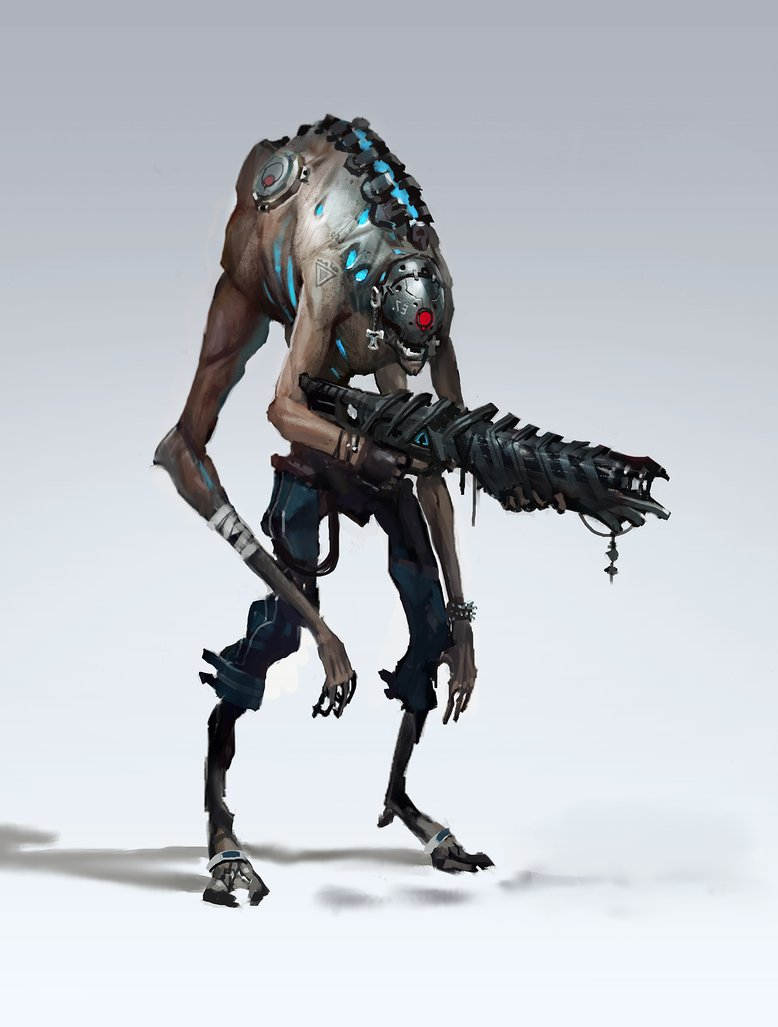
\includegraphics[width=\linewidth]{soldier_by_zoonoid-d4qf4cg}

\begin{redtable}{\linewidth}{@{}L{.35}@{}L{.65}@{}}
  \textbf{Singular} & Pluv\\
  \textbf{Plural} & Pluvma\\
  \textbf{Height} & 150-200cm\\
  \textbf{Weight} & 55-115kg\\
  \textbf{Gender Ratio} & 80\% Male / 20\% Female\\
  \textbf{Reproduction} & Viviparity (Live birth)\\
  \textbf{Maturity} & 20 years\\
  \textbf{Diet} & Omnivore\\
  \textbf{Homeworld} & Reistus (Lost)\\
\end{redtable}

The Pluvma are a multi-limbed alien species that is considered curious and quirky. They are as tall and weigh about the same as a human, with most of their mass located on the top half of their body. They have four arms that are each as functional as a humans, allowing a Pluvmian to manipulate more things at once. Even with the extra arms, the Pluvma only have a single eye which means they have trouble with depth perception.

Females in Pluvma society are generally rare, so males generally have to stand out from the pack to attract the opposite sex. This has resulted in Pluvmian society revolving around discovering something new and different, and if the Pluvmian male cannot they default to \textit{being} something new and different. It is because of this that no two Pluvmian males will ever purposely act alike.

To create a Pluvmian character, please refer to the \textit{\hyperref[sec:rules-creation]{Character creation section}}

\textbf{Pluvmian Male Names:}

Abbagan, Buckia, Bundamerrie, Chiridie, Coolanyarra, Doontah, Coombooloo, Jiwabiddy, Kagageerra, Mongah, Moolyal, Morangoril, Nangerow, Narga, Painbiddy, Tumbunna, Unjung, Wobbing, Yabongona, Yulla

\textbf{Pluvmian Female Names:}

Bobong, Booyo, Bringie, Chacca, Cookal, Dongo, Hynman, Inyah, Junman, Kurra, Milla, Noggo, Noothy, Nowen, Ronga, Tubar, Ula, Wisney, Woodya, Yanyea

\textbf{Secondary Names:}

Anakaus, Bisahalani, Degotoga, Espowyes, Gawonish, Harkahome, Hesutuvito, Keezheekoni, Kusinut, Lenmana, Mantotohpa, Matchitehew, Melkedoodum, Ocunnohurst, Ojinjintka, Quahneah, Sikyatavo, Taregan, Wawetseka, Wokaihwoko

  \columnbreak
  \subsection{Human}
\label{sec:specie-human}

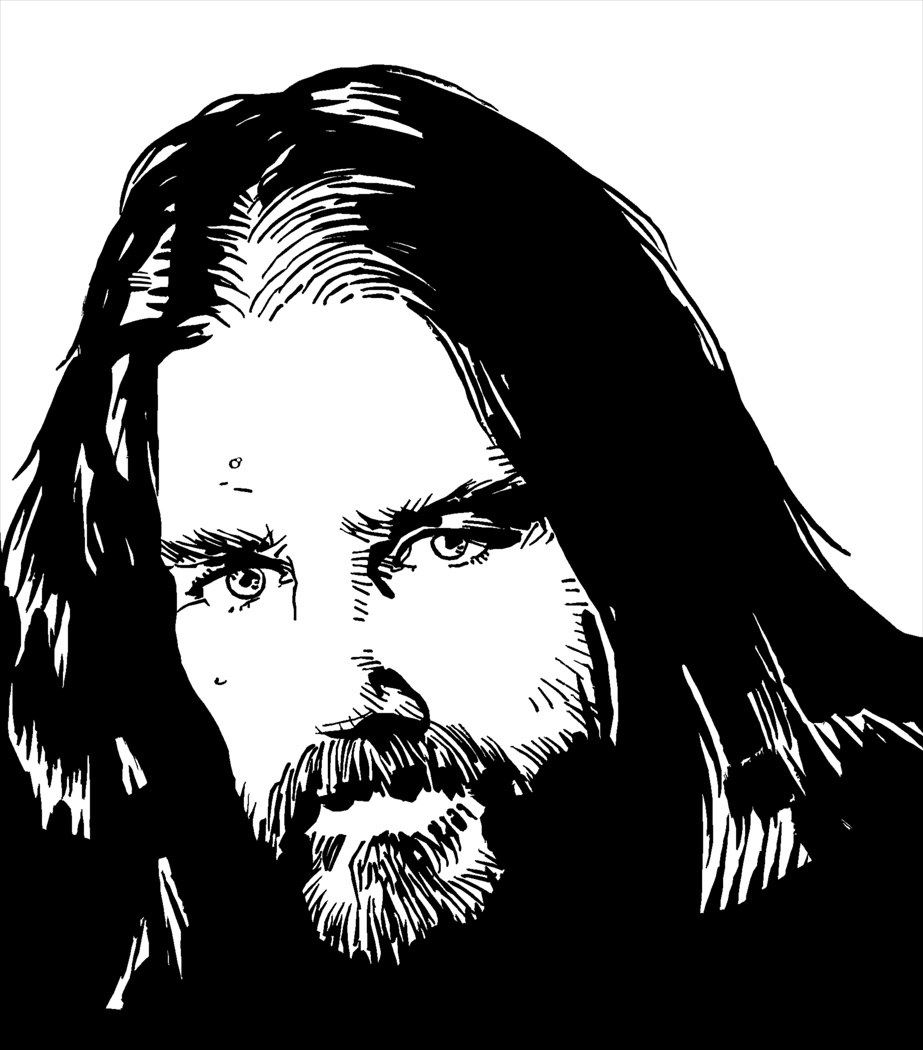
\includegraphics[width=\linewidth]{TCP-Pirate-2}

\begin{redtable}{\linewidth}{@{}L{.35}@{}L{.65}@{}}
  \textbf{Singular} & Terran / Human\\
  \textbf{Plural} & Terrans / Humans\\
  \textbf{Height} & 150-200cm\\
  \textbf{Weight} & 55-115kg\\
  \textbf{Gender Ratio} & 50\% Male / 50\% Female\\
  \textbf{Reproduction} & Viviparity (Live birth)\\
  \textbf{Maturity} & 18 years\\
  \textbf{Diet} & Omnivore\\
  \textbf{Homeworld} & Earth\\
\end{redtable}

There are various types of humans seen in the Black. Some are proud of their genetic lineage tracing all the way back to Sol. Others are escaped clones that were destined to be uploaded with someone else's cortical stack. Even more are genetically altered humans, designed for the specific conditions of their colony during the Pre-Surge days. All of these different varieties, no matter how weird or alien, are still considered human.

To create a Human character, please refer to the \textit{\hyperref[sec:rules-creation]{Character creation section}}

  \columnbreak
  \subsection{Uplifted}
\label{sec:specie-uplifted}

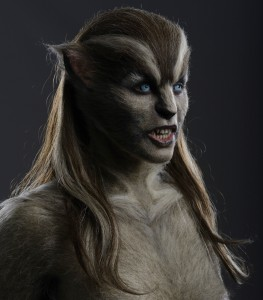
\includegraphics[width=\linewidth]{wolves-movie-still-1-263x300}

Uplifted is the general name given to the genetically-engineered animals that have been given basic sentience and humanoid features. The original reason behind this science experiment has long been lost, but many tech-heads speculate that the Uplifted were supposed to perform the menial labour on planets that could not support a Bot network. Regardless, the Uplifted are still treated as an inferior species because of their artificial evolution.

Uplifted physically range wildly across the spectrum from humanoid to their base animal form, but all Uplifted have at least a humanoid-style torso that have two arms with opposable thumbs (for manipulating objects). Faces may or may not have a prominent snout, and some uplifted do not have a tail. Almost all Uplifted have the fur coat of their base animal base form, but some choose to partially shave or style it to better fit in humanoid society.

Due to their severe genetic alteration and base animal genetics, Uplifted cannot breed with humans or with their animal predecessors. This does not deter kinky humanoids, and many unsavoury places in the Black offer "special" Uplifted services. However the heart wants what it wants, and Uplifted-Human couples are a rare sight in the Black. These couples generally seek out geneticists who are able to splice their DNA into viable offspring.

To create an Uplifted character, please refer to the \textit{\hyperref[sec:rules-creation]{Character creation section}}

\end{multicols}

  % Hindrances
  % =================
% Hindrances
% =================
\section{Hindrances}

Hindrances are traits that affect your character negatively during the game. Some will affect your rolls, while others will affect the way you role-play. You are encouraged to come up with backstory for each hindrance; feel free to rename a hindrance to better suit your character concept.

When your character "levels up" by earning an advance, you can use that advance to "buy off" or remove one hindrance. A hindrance cannot be removed in any other way. For example, if you choose the \textit{Blind} hindrance then you cannot purchase cyber-eyes to remove the hindrance. Instead, your cyber-eyes malfunction in a way to satisfy the \textit{Blind} condition (you can flavour it to be that your blindness has something to do with your brain).

\subsection{Background}

\begin{redpowertable}{@{}p{.25\linewidth}@{}p{.10\linewidth}@{}p{.65\linewidth}@{}}
\textbf{Name}     & \textbf{Type}  & \textbf{Description}\\
All Thumbs        & \textit{Minor} & You are naturally clumsy. -2 penalty to Repair, and a natural 1 on the skill die (regardless of wild die) causes a malfunction\\
Bad Luck          & \textbf{Major} & Bad things always seem to happen to you. One less Benny per session\\
Clueless          & \textbf{Major} & -2 to most Common Knowledge rolls\\
Elderly           & \textbf{Major} & -1 to Pace, and -1 Strength and Vigor die types (Cannot go lower than a d4, but this penalty applies during character advancement). +5 skill points to use on any Smarts skills\\
Enemy             & \textit{Minor} / \textbf{Major} & You have a recurring Nemesis. \textit{Minor} is a lone gunslinger, while \textbf{Major} is someone with serious resources\\
Illiterate        & \textit{Minor} & You are unable to read or write\\
Low-Tech          & \textit{Minor} / \textbf{Major} & You are from a Low-Tech world. -2 penalty when using technological devices not of your own Tech-Level (-4 penalty as a \textbf{Major})\\
Outsider          & \textit{Minor} & You are a social outcast. -2 Charisma and treated badly by mainstream society\\
Poverty           & \textit{Minor} & You can never hold onto your money. Halve your starting funds, and halve your money every in-game week\\
Slow-witted       & \textit{Minor} / \textbf{Major} & -2 Penalty to one type of Trick (Smarts or Agility). As a \textbf{Major}, you suffer a penalty to both\\
Wanted            & \textit{Minor} / \textbf{Major} & You are a criminal of some sort. The severity of the crime determines the type\\
Young             & \textbf{Major} & You are a pre-teen for your race. -3 points for Attributes, -10 points for Skills, but you get an extra +1 Benny per session. Once you have matured you do not need to buy off the Hindrance, but you do lose the extra Benny\\
\end{redpowertable}

\subsection{Personality}

\begin{redpowertable}{@{}p{.25\linewidth}@{}p{.10\linewidth}@{}p{.65\linewidth}@{}}
\textbf{Name}     & \textbf{Type}  & \textbf{Description}\\
Arrogant          & \textbf{Major} & Must humiliate an opponent (i.e. disarm then hand weapon back), and will always challenge the "leader"\\
Big Mouth         & \textit{Minor} & Unable to keep a secret, and blabs at the worst time\\
Cautious          & \textit{Minor} & You are overly careful\\
Code of Honour    & \textbf{Major} & You keep your word and act like a gentleman at all times\\
Curious           & \textbf{Major} & You must know everything, and wants to know what is behind a potential mystery\\
Death Wish        & \textit{Minor} & You want to die after completing a certain task or goal\\
Delusional        & \textit{Minor} / \textbf{Major} & \textit{Minor} delusions are harmless, while \textbf{Major} are ones that you express frequently and could lead to danger\\
Expensive Taste   & \textit{Minor} & For some reason your character is obsessed with brand-names. Whenever you buy equipment, you pay 25\% more\\
Greedy            & \textit{Minor} / \textbf{Major} & \textit{Minor} means you argue blithely over loot, while \textbf{Major} is fighting over anything considered unfair\\
Habit             & \textit{Minor} / \textbf{Major} & -1 Charisma, and Fatigue roll is required when deprived of \textbf{Major} habit\\
Heavy Sleeper     & \textit{Minor} & Your sleep deeply, and takes a -4 penalty to Notice when asleep\\
Hedonistic        & \textit{Minor} & You enjoy the finer things in life and enjoy them as much as possible, and may not take the current task at hand seriously if there is nearby excess to indulge in\\
Heroic            & \textbf{Major} & You always help those in need, no matter the personal risk\\
Insomnia          & \textit{Minor} & When attempting to fall asleep you must make a Spirit roll. Failure means you do not get a good night's sleep and suffer 1 point of Fatigue. Purchasing appropriate medication give a +2 bonus to the Spirit roll\\
Loyal             & \textit{Minor} & You never betray or disappoint your friends and allies\\
Machine-man       & \textit{Minor} & You fanatically believe that cyberware is the future. -2 Charisma when dealing with organics without cyberware\\
Manic             & \textbf{Major} & You never take the time to consider your actions. You cannot Aim or make Called Shots, or any other actions that require patience and considered action (GM's discretion). You also expend double the ammunition\\
Mean              & \textit{Minor} & -2 to Charisma for being ill-tempered and surly\\
Next-Gen          & \textbf{Minor} & (Requires Cyberware). You crave the latest hardware and squeeze the best performance out of your cyberware. You constantly spend money on upgrades, polish and decorative decals. Halve your money every in-game week.\\
Old School        & \textbf{Major} & You distrust and abhor computers, cyberware and the unnatural. -2 Charisma when dealing with Bots, Ghosts or anyone with cyberware. If you get Cyberware yourself, you are limited to only half of the maximum charges (e.g 5 instead of 10 charges)\\
Overconfident     & \textbf{Major} & You believe you can do anything\\
Pacifist          & \textit{Minor} / \textbf{Major} & \textit{Minor} means you only fight in self-defence. \textbf{Major} means you will never hurt another living being\\
Panicky           & \textbf{Major} & If you are dealt a Jack or higher, you must redraw until you get lower than a Jack. This does not apply to Jokers\\
Phobia            & \textit{Minor} / \textbf{Major} & When near the source of the phobia, -2 (\textit{Minor}) or -4 (\textbf{Major}) to all Trait rolls\\
Prideful          & \textit{Minor} & You just don’t know when to brag and when to act. Your first round in any combat must be spent announcing how great you are, or pronouncing the doom of those who oppose you. If for some reason you must act instead, it costs you a Benny\\
Quirk             & \textit{Minor} & You have a \textit{Minor} but persistent foible\\
Show-off          & \textit{Minor} & You are more concerned with your graceful composure and adding stylish flourishes during combat than inflicting the most damage possible. -2 to all damage rolls\\
Stubborn          & \textit{Minor} & You always want your own way\\
Unfocused         & \textbf{Major} & Your Wild Die is a d4 instead of a d6. When you spend a Benny, your Wild Die is a d6 for that particular roll\\
Vengeful          & \textit{Minor} / \textbf{Major} & You hold a grudge; \textbf{Major} means you will kill over that grudge\\
Vow               & \textit{Minor} / \textbf{Major} & A pledge to a group, deity, or religion. (It's type depends on the vow)\\
Xenophobe         & \textit{Minor} / \textbf{Major} & As a \textit{Minor} Hindrance you suffer a -2 Charisma modifier when dealing with other races, or if your intolerance is known by others. The penalty is -4 as a \textbf{Major} Hindrance\\
Yellow            & \textbf{Major} & You are squeamish at the sight of blood. -2 to all fear-based Spirit checks\\
\end{redpowertable}

\subsection{Physical}

\begin{redpowertable}{@{}p{.25\linewidth}@{}p{.10\linewidth}@{}p{.65\linewidth}@{}}
\textbf{Name}     & \textbf{Type}  & \textbf{Description}\\
Anemic            & \textit{Minor} & Prone to sickness/disease/fatigue. -2 from all Fatigue checks (including those to resist poison and disease)\\
Bad Eyes          & \textit{Minor} & -2 to attack or notice more than 5 squares away (unless wearing glasses)\\
Blind             & \textbf{Major} & -6 to all tasks that require vision, and -2 to social tasks (as you cannot 'read' the person). Gain a free Edge\\
Cyberware Intolerance & \textit{Minor} & (Organic only) Cannot install any cyberware, including simple AR, prosthetic limbs or Cortical Stacks\\
FTL Sickness      & \textit{Minor} & After each use of FTL travel, you suffer a level of Fatigue that takes 24 hours to fade.\\
Hard of Hearing   & \textit{Minor} / \textbf{Major} & \textit{Minor} is -2 to Notice checks based on sounds; \textbf{Major} is completely Deaf (automatic failure)\\
Lame              & \textbf{Major} & -2 Pace and running die is a d4\\
Obese             & \textit{Minor} & +1 Toughness, -1 Pace, d4 Running die\\
One Arm           & \textbf{Major} & -4 to tasks requiring two arms\\
One Eye           & \textbf{Major} & -1 to Charisma if not wearing some kind of eye patch; -2 to rolls that require depth perception such as Shooting\\
One Leg           & \textbf{Major} & Pace is 2 and cannot run, -2 to Trait rolls that require mobility such as Fighting, and -2 to all Athletic rolls\\
Small             & \textbf{Major} & -1 Size. This gives you a -1 penalty to Toughness and affects to-hit attack rolls\\
Small Frame       & \textit{Minor} & You have a very slight build, reducing your carrying capacity. May only carry 2 x your Strength die unencumbered\\
Ugly              & \textit{Minor} & -2 to Charisma due to appearance\\
Zero-G Sickness   & \textbf{Major} & You automatically gain a level of Fatigue when you in Zero-G and not restrained in some way. Recovered after one hour in gravity\\
\end{redpowertable}

  % Edges
  % =================
% Edges
% =================

\section{Edges}

\begin{multicols}{2}

%
% Background Edges
%
\subsection{Background Edges}

\begin{genericsection}{Alertness (Novice)}
+2 bonus to Notice rolls to hear, see, or otherwise sense the world around you.
\end{genericsection}

\begin{genericsection}{Ambidextrous (Novice)}
\textbf{Requirements: Agility d8+}\\
Characters normally suffer a -2 penalty when using their off-hand. You ignore this penalty
\end{genericsection}

\begin{genericsection}{Attractive (Novice)}
\textbf{Requirements: Vigor d6+}\\
+2 bonus to Charisma for being so goddamn handsome
\end{genericsection}

\begin{genericsection}{Attractive - Improved (Novice; Attractive)}
\textbf{Requirements: Attractive}\\
Similar to Attractive but with a +4 bonus to Charisma
\end{genericsection}

\begin{genericsection}{Brave (Novice)}
\textbf{Requirements: Spirit d6+}\\
+2 bonus to all Fear tests
\end{genericsection}

\begin{genericsection}{Brawny (Novice)}
\textbf{Requirements: Strength d6+; Vigor d6+}\\
+1 bonus to Toughness; Encumbrance is now 5 x Strength in kilograms (instead of 3 x Strength)
\end{genericsection}

\begin{genericsection}{Fast Healer (Novice)}
\textbf{Requirements: Vigor d8+}\\
+2 bonus to Vigor rolls when checking for natural healing
\end{genericsection}

\begin{genericsection}{Fleet footed (Novice)}
\textbf{Requirements: Agility d8+}\\
+2 bonus to Pace and roll a d10 when running instead of a d6
\end{genericsection}

\begin{genericsection}{Linguist (Novice)}
\textbf{Requirements: Smarts d6+}\\
Knows a number of languages equal to their Smarts die, and can make a Smarts roll with a -2 penalty to make themselves understood in a language they have heard spoken for at least a week
\end{genericsection}

\begin{genericsection}{Gifted (Novice)}
Gain +1 Benny at the start of a new game session
\end{genericsection}

\begin{genericsection}{Gifted - Improved (Novice)}
\textbf{Requirements: Gifted}\\
Same as Gifted but gain +2 Bennies at the start of each session instead
\end{genericsection}

\begin{genericsection}{Graduate (Novice)}
\textbf{Requirements: Smarts d8+}\\
Has an additional 4 skill points to spend on any Smarts-related skills. At least one of these must be a Knowledge skill at d6 or better (their Major)
\end{genericsection}

\begin{genericsection}{Hacker (Novice)}
\textbf{Requirements: Smarts d8+; Investigation d6+, Security d8+}\\
+2 bonus to all Investigation rolls when using a computer and +2 on security rolls when hacking a computer
\end{genericsection}

\begin{genericsection}{Intuition (Novice)}
\textbf{Requirements: Spirit d8+}\\
Spend a Benny and make a Spirit roll; if successful, you may ask the GM a single, simple question. The GM must either give you a simple answer or return your Benny.
\end{genericsection}

\begin{genericsection}{Luck (Novice)}
Lady Luck often smiles on you. Whenever you spend a Benny, roll a d6. On a 6, you get the Benny back immediately (it may even be spent on the same roll they spent the first one on).
\end{genericsection}

\begin{genericsection}{One of a Kind (Novice)}
You are from a unique species not found anywhere else in the known Black. The Black is vast and alien migration was common before the Surge, so some aliens have unfortunately become stranded far from home. You gain +2 Charisma because everyone is wondering what exactly you are.
\end{genericsection}

\begin{genericsection}{Photographic Memory (Novice)}
\textbf{Requirements: Smarts d8+}\\
You gain a +2 bonus on Common Knowledge rolls, and on Smarts rolls made to remember something
\end{genericsection}

\begin{genericsection}{Privileged (Novice)}
You grew up rich or as part of a famous family. This can give you a lot of perks, but it also have lots of responsibilities. You gain the "Rich" Edge for free (cannot chose "Rich" again while you have "Privileged") as well as a +2 Charisma bonus. To balance this out, you have many responsibilities. You have teams of workers under your control, as well as land, family home, and other assets. All of this must be determined by the GM, and balanced by the grave responsibilities you face. This includes managing aspects of the family business, dealing with jealous rivals, taking out time to appease fans, and constant other plots
\end{genericsection}

\begin{genericsection}{Psionic Resistance (Novice)}
\textbf{Requirements: Spirit d8+}\\
Add 2 points of Armour when hit by damage caused by Psionic powers, and add a +2 bonus to Trait rolls when resisting opposing psionic powers. This includes friendly psionic powers
\end{genericsection}

\begin{genericsection}{Psionic Resistance - Improved (Novice)}
\textbf{Requirements: Psionic Resistance}\\
Similar as above but Armour and resistance bonuses are increased to +4
\end{genericsection}

\begin{genericsection}{Quick (Novice)}
\textbf{Requirements: Agility d8+}\\
If you are dealt a 5 or lower, you must redraw until you get higher than a 5
\end{genericsection}

\begin{genericsection}{Rich (Novice)}
Start with 3 times the normal starting funds
\end{genericsection}

\begin{genericsection}{Rich - Improved (Novice)}
\textbf{Requirements: Rich}\\
Start with 7 times the normal starting funds
\end{genericsection}

%
% Combat Edges
%
\subsection{Combat Edges}

\begin{genericsection}{Block (Seasoned)}
\textbf{Requirements: Fighting d8+}\\
+1 bonus to Parry
\end{genericsection}

\begin{genericsection}{Block - Improved (Veteran)}
\textbf{Requirements: Block}\\
+2 to Parry
\end{genericsection}

\begin{genericsection}{Brawler (Novice)}
\textbf{Requirements: Strength d8+}\\
+2 bonus to unarmed damage rolls
\end{genericsection}

\begin{genericsection}{Bruiser (Seasoned)}
\textbf{Requirements: Brawler}\\
When you get a raise on unarmed Fighting, roll a d8 instead of a d6
\end{genericsection}

\begin{genericsection}{Combat Reflexes (Seasoned)}
+2 bonus to Spirit rolls when attempting to recover from being Shaken
\end{genericsection}

\begin{genericsection}{Counterattack (Seasoned)}
\textbf{Requirements: Fighting d8+}\\
Once per round (if not Shaken), get one free Fighting attack against one adjacent foe who failed a Fighting attack against you. This attack has a -2 Penalty, must be a normal attack, and may not be combined with Frenzy, Sweep or Full Defense
\end{genericsection}

\begin{genericsection}{Counterattack - Improved (Veteran)}
\textbf{Requirements: Counterattack}\\
As above but ignore the -2 penalty
\end{genericsection}

\begin{genericsection}{Covered (Novice)}
\textbf{Requirements: Smarts d6+}\\
While in cover, foes suffer a –1 penalty to any physical attack rolls. The hero also adds +1 to their Toughness against area effect damage as long as they are prone or in cover
\end{genericsection}

\begin{genericsection}{Covered - Improved (Seasoned)}
\textbf{Requirements: Covered}\\
As Covered, but foes subtract 2 from attack rolls, and the hero gains +2 Toughness versus area effect attacks if prone or in cover.
\end{genericsection}

\begin{genericsection}{Die Hard (Novice)}
\textbf{Requirements: Vigor d6+}\\
+1 bonus to Toughness when at three Wounds
\end{genericsection}

\begin{genericsection}{Dodge (Seasoned)}
\textbf{Requirements: Agility d8+}\\
-1 penalty to opponent's ranged attack rolls (unless you are surprised), and add +1 to Agility roll to evade area effect
\end{genericsection}

\begin{genericsection}{Dodge - Improved (Veteran)}
\textbf{Requirements: Dodge}\\
As above but opponent subtracts a -2 penalty from their ranged attack roll, and add +2 to Agility roll to evade a ranged area effect
\end{genericsection}

\begin{genericsection}{Élan (Novice)}
\textbf{Requirements: Spirit d8+}\\
When you spend a Benny on a trait roll (including a soak roll), add +2 to the final total
\end{genericsection}

\begin{genericsection}{Extraction (Novice)}
\textbf{Requirements: Agility d8+}\\
Make an Agility roll when moving away from an adjacent opponent. On a success, one opponent does not get a free attack when you disengage
\end{genericsection}

\begin{genericsection}{Extraction - Improved (Novice)}
\textbf{Requirements: Extraction}\\
As above, but with a raise all opponents loose their free attack when you disengage
\end{genericsection}

\begin{genericsection}{First Strike (Novice)}
\textbf{Requirements: Agility d8+}\\
Once per round you get a free Fighting attack action against a single opponent who moves adjacent to you. This automatically interrupts opponents action, and does not cost you your action
\end{genericsection}

\begin{genericsection}{First Strike - Improved (Heroic)}
\textbf{Requirements: First Strike}\\
As above but you make a free Fighting attack against each and every opponent who moves adjacent to you
\end{genericsection}

\begin{genericsection}{Frenzy (Seasoned)}
\textbf{Requirements: Fighting d10+}\\
You make an extra Fighting attack per round when you take one Fighting attack this turn, with all attacks having a -2 penalty
\end{genericsection}

\begin{genericsection}{Frenzy - Improved (Veteran)}
\textbf{Requirements: Frenzy}\\
As above, but without the -2 Frenzy penalty
\end{genericsection}

\begin{genericsection}{Giant Killer (Veteran)}
You gain a bonus +1d6 damage when attacking creatures 3 times larger than yourself
\end{genericsection}

\begin{genericsection}{Hard to Kill (Novice)}
\textbf{Requirements: Spirit d8+}\\
When forced to make a Vigor rolls due to Incapacitation, you may ignore Wound modifiers
\end{genericsection}

\begin{genericsection}{Harder to Kill (Veteran)}
\textbf{Requirements: Hard to Kill}\\
If you are "killed", roll a die. On an odd result you are dead as usual. On an even roll, you are incapacitated but somehow escapes death.
\end{genericsection}

\begin{genericsection}{Improvisational Fighter (Seasoned)}
\textbf{Requirements: Smarts d6+}\\
You do not suffer the -1 penalty to Parry and attack when using improvised weapons
\end{genericsection}

\begin{genericsection}{Killer Instinct (Heroic)}
You don’t like to lose. On ties for any opposed roll of any sort, you win. In addition, if your skill die on an opposed skill roll is a 1, you can re-roll it (but must keep the second result, even if it’s another 1)
\end{genericsection}

\begin{genericsection}{Level Headed (Seasoned)}
\textbf{Requirements: Smarts d6+}\\
Draw an additional Action card in combat and act on the best of the draw
\end{genericsection}

\begin{genericsection}{Level Headed - Improved (Seasoned)}
\textbf{Requirements: Level Headed}\\
As above, but draw 3 cards instead
\end{genericsection}

\begin{genericsection}{Marksman (Seasoned)}
If you do not move, you can fire as if you took the Aim action. This edge cannot be used with a Rate of Fire greater than 1
\end{genericsection}

\begin{genericsection}{Martial Artist (Novice)}
\textbf{Requirements: Fighting d6+}\\
You are never considered Unarmed and so do not suffer the Unarmed Defender rule. Add a bonus +d4 damage to your Strength roll
\end{genericsection}

\begin{genericsection}{Martial Artist - Improved (Veteran)}
\textbf{Requirements: Martial Artist, Fighting d10+}\\
You add a bonus +d6 to your unarmed damage
\end{genericsection}

\begin{genericsection}{Nerves of Steel (Novice)}
\textbf{Requirements: Vigor d8+}\\
You ignore 1 point of Wound penalties
\end{genericsection}

\begin{genericsection}{Nerves of Steel - Improved (Novice)}
\textbf{Requirements: Nerves of Steel}\\
You ignore 2 points of Wound penalties
\end{genericsection}

\begin{genericsection}{No Mercy (Seasoned)}
You may spend a Benny to re-roll any one damage roll, including those for area effects
\end{genericsection}

\begin{genericsection}{Quick Draw (Novice)}
\textbf{Requirements: Agility d8+}\\
Allows you to draw a weapon as a free action (and avoid the -2 multi-action penalty if you want to fire as well). If you must make an Agility roll to draw your weapon, add +2 to that roll
\end{genericsection}

\begin{genericsection}{Resilient (Novice)}
\textbf{Requirements: Vigor d8+}\\
You are thick as a brick or have the heart of a lion. When any damaging attack creates a Shaken condition with no accompanying wounds you may make a free Soak roll. On a Raise the Shaken condition is removed. If unsuccessful a Benny may still be paid to immediately eliminate the Shaken penalty
\end{genericsection}

\begin{genericsection}{Rock and Roll (Seasoned)}
\textbf{Requirements: Shooting d8+}\\
If you do not move, ignore the recoil penalty for firing a weapon on full automatic
\end{genericsection}

\begin{genericsection}{Trademark Spacecraft (Novice)}
\textbf{Requirements: Piloting d8+, Repair d8+, Shooting d8+}\\
You know your spacecraft like the back of your hand, and then some. When using one specific spacecraft, you gain a +1 bonus to Piloting, Repair, and Shooting rolls. A character may take this Edge multiple times, but each time it must be applied to a different spacecraft. If a Trademark Spacecraft is destroyed, stolen, or otherwise permanently removed from the game,
the hero can switch this Edge to another craft, but it takes two weeks for the Edge to kick in
\end{genericsection}

\begin{genericsection}{Trademark Spacecraft - Improved) (Veteran)}
\textbf{Requirements: Trademark spacecraft}\\
As above, but the bonus is now +2
\end{genericsection}

\begin{genericsection}{Trademark weapon (Novice)}
\textbf{Requirements: Fighting or Shooting d10+}\\
You know one unique weapon intimately. When using that weapon, add +1 to Fighting or Shooting rolls. You can take this edge multiple times for different weapons. If the weapon is lost, you can replace it but it takes 2 in-game weeks to be attuned to it
\end{genericsection}

\begin{genericsection}{Trademark weapon - Improved (Veteran)}
\textbf{Requirements: Trademark weapon}\\
As above, but the bonus is +2
\end{genericsection}

\begin{genericsection}{Two-Fisted (Novice)}
\textbf{Requirements: Agility d8+}\\
You are not ambidextrous, you just know how to fight with two weapons at once. When attacking with a weapon in each hand, roll each attack separately but ignore the multi-attack penalty
\end{genericsection}

%
% Leadership Edges
%
\subsection{Leadership Edges}

\begin{genericsection}{Command (Novice)}
\textbf{Requirements: Smarts d6+}\\
All nearby allies within 5 squares of you gain a bonus +1 to Shaken rolls
\end{genericsection}

\begin{genericsection}{Command Presence (Novice)}
\textbf{Requirements: Command}\\
You have a command radius of 10 squares instead of 5
\end{genericsection}

\begin{genericsection}{Fervor (Veteran)}
\textbf{Requirements: Command, Spirit d8+}\\
You are an inspiration to your men, giving allies within your command radius a +1 to Fighting damage rolls
\end{genericsection}

\begin{genericsection}{Hold the Line (Seasoned)}
\textbf{Requirements: Command, Smarts d8+}\\
Gives allies within your command radius a +1 to Toughness
\end{genericsection}

\begin{genericsection}{Inspire (Seasoned)}
\textbf{Requirements: Command}\\
As in Command, but +2 to Shaken rolls
\end{genericsection}

\begin{genericsection}{Leader of Men (Veteran)}
\textbf{Requirements: Command}\\
Allies under your command roll a d10 instead of a d6 when making group rolls
\end{genericsection}

\begin{genericsection}{Natural Leader (Novice)}
\textbf{Requirements: Command, Spirit d8+}\\
You may share your Bennies with any troops under your command
\end{genericsection}

\begin{genericsection}{Tactician (Seasoned)}
\textbf{Requirements: Smarts d8+, Battle d6+, Command}\\
At the beginning of a fight and before any initiative cards are dealt, you makes a Battle roll. For each success and raise you receive one initiative card. These are kept separate from your regular initiative cards and are not placed back into the deck until used or the combat ends. At the start of any round, you may give one or more of these extra cards to allies, who then use it as their initiative card for the round in place of the one dealt them. This allows Extras to operate independently of Wild Card characters for one round if they receive their own card. Only one character per encounter may use this Edge
\end{genericsection}


%
% Professional Edges
%
\subsection{Professional Edges}

\begin{genericsection}{Ace (Novice)}
\textbf{Requirements: Agility d8+}\\
Special pilots and drivers. Add +2 to Driving and Piloting rolls. In addition, you may spend Bennies to make soak rolls for any vehicle or vessel you control. This is a Driving or Piloting roll at -2 (cancelling out their bonus +2). Each success and raise negates a wound and any critical hit that would have resulted
\end{genericsection}

\begin{genericsection}{Bounty Hunter (Seasoned)}
\textbf{Requirements: Smarts d6+, Survival d6+, Streetwise d6+}\\
+2 to all Survival, Streetwise, and Knowledge rolls relating to their current bounty, +1 Intimidation
\end{genericsection}

\begin{genericsection}{Diplomat (Seasoned)}
\textbf{Requirements: Smarts d6+, Insight d6+, Persuasion d8+}\\
+2 on persuasion rolls and +2 on insight rolls, +1 on reaction table rolls
\end{genericsection}

\begin{genericsection}{Explorer (Novice)}
\textbf{Requirements: Smarts d8+, Natural Sciences at d8+}\\
+2 on Natural Sciences skill. +2 to survival and vigor checks while “in the field”
\end{genericsection}

\begin{genericsection}{Gravity Acclimation (Novice)}
\textbf{Requirements: Agility d6+}\\
Ignore the -2 penalty incurred due to working in different gravity.
\end{genericsection}

\begin{genericsection}{Navigator (Novice)}
\textbf{Requirements: Smarts d6+, Astrogation d8+}\\
+2 on Astrogation for FTL Travel, +1 for all other Navigation rolls. Saves d6 travel-time (in base unit of time)
\end{genericsection}

\begin{genericsection}{Healer (Novice)}
\textbf{Requirements: Spirit d8+}\\
Add +2 to all Healing rolls (including natural healing). Up to five companions travelling add the bonus to their natural healing as well
\end{genericsection}

\begin{genericsection}{Reclaimer (Novice)}
\textbf{Requirements: Smarts d6+, Repair d6+}\\
+2 on Common Knowledge rolls to identify or value a find. +1 to any repair rolls on scavenged objects
\end{genericsection}

\begin{genericsection}{Researcher (Novice)}
\textbf{Requirements: Smarts d6+}\\
+2 to all Science-based knowledge checks
\end{genericsection}

\begin{genericsection}{Smuggler (Novice)}
\textbf{Requirements: Piloting d6+, Persuasion d6+}\\
+2 to persuasion rolls when speaking to Law Enforcement officials, +2 on piloting when trying to stay undetected
\end{genericsection}

\begin{genericsection}{Survival Training (Novice)}
\textbf{Requirements: Appropriate background}\\
You have graduated from a Ranger School or a very similar facility. You gain +2 to all Fatigue rolls made against environmental hazards (including cold, heat, and sleep), and +2 to all Survival rolls. Also, you make Vigor rolls every 18 hours for sleep deprivation, instead of the standard 12 hours
\end{genericsection}


%
% Social Edges
%
\subsection{Social Edges}

\begin{genericsection}{Battle Brothers (Veteran)}
\textbf{Requirements: Common Bond}\\
This group has been to Hell and back together. That kind of bond hardens people, making them able to withstand wounds that might otherwise put them out of action. Increase Toughness by +1 for each other “brother” within 6" (12 yards), to a maximum of +4
\end{genericsection}

\begin{genericsection}{Charismatic (Novice)}
\textbf{Requirements: Spirit d8+}\\
+2 bonus to Charisma
\end{genericsection}

\begin{genericsection}{Common Bond (Novice)}
\textbf{Requirements: Spirit d8+}\\
Signifies a special link between close companions (whether or not they get along). You may freely give your Bennies to any other player you can communicate with
\end{genericsection}

\begin{genericsection}{Connections (Novice)}
You know someone on the inside of a large organization of your choice. This can be taken multiple times, but only once per organization. To use a Connection, you need to get in touch with them (Streetwise roll) and then convince them to help (Persuasion roll). On a success, they help without putting themselves at risk. With a raise, the connection is willing to leak sensitive information but stops short of outright betrayal. On two or more raises, you can expect serious help (including financial). If you require muscle, the contact delivers one expert or five average henchmen
\end{genericsection}

\begin{genericsection}{Fence (Novice)}
\textbf{Requirements: Smarts d8+, Streetwise d8+}\\
On a successful Streetwise roll your finds a buyer willing to pay 50\% of the gear’s value. A
raise increases this to 75\%
\end{genericsection}
 
\begin{genericsection}{Smooth Talker (Novice)}
\textbf{Requirements: Persuasion d6+}\\
+2 to Persuasion rolls
\end{genericsection}

\begin{genericsection}{Strong Willed (Novice)}
\textbf{Requirements: Intimidation d6+, Taunt d6+}\\
Add +2 to Intimidation and Taunt rolls, as well as Spirit and Smarts rolls when resisting Test of Wills attacks
\end{genericsection}

%
% Weird Edges
%
\subsection{Weird Edges}

\begin{genericsection}{AR power user (Novice)}
\textbf{Requirements: Smarts d8+}\\
+1 bonus to all AR-related rolls, and you can control your Muse voicelessly
\end{genericsection}

\begin{genericsection}{Beast Master (Novice)}
\textbf{Requirements: Psionic Background, Spirit d8+}\\
Creatures like you, and won't attack you unless you attack them first or they are enraged. You also have attracted a loyal animal companion of some sort, with an empathetic connection. If the companion is killed, you bond with a replacement in 2d6 days
\end{genericsection}

\begin{genericsection}{Cyberware charges (Novice)}
\textbf{Requirements: Cyberware install}\\
This grants you an extra 5 power charges for all cyberware you have. May be selected more than once, but only once per rank
\end{genericsection}

\begin{genericsection}{Cyberware install (Novice)}
\textbf{Requirements: Spirit d6+, Vigor d6+}\\
Allows the use of Enhanced Cyberware (see \textit{Cyberware}). You can change this cyberware at any time (at a cost). You have a limit of one cyberware install.
\end{genericsection}

\begin{genericsection}{Cyberware (New) (Novice)}
\textbf{Requirements: Cyberware Install}\\
Increase your cyberware limit by one. You can change this cyberware at any time (at a cost).
\end{genericsection}

\begin{genericsection}{Danger Sense (Novice)}
\textbf{Requirements: Psionic Background}\\
(Organic only) You can sense when something bad is about to happen. When you are the victim of a surprise attack, ambush, or other nasty surprise, you get a Notice roll at -2 just before the event. If successful, you know something is about to happen and may take appropriate action against it. You are on Hold for the first round. If you fail, you follow normal Surprise rules
\end{genericsection}

\begin{genericsection}{Psionic Background (Novice)}
\textbf{Requirements: Psionics d6+}\\
(Organic only) Allows the use of psionic abilities (see \textit{Psionics})
\end{genericsection}

\begin{genericsection}{Psionic (New) (Novice)}
\textbf{Requirements: Psionic Background}\\
(Organic only) Learn a new psionic ability
\end{genericsection}

%
% Legendary Edges
%
\subsection{Legendary Edges}

\begin{genericsection}{Followers (Legendary)}
5 devoted followers join you. They must have some way to work and earn income, and generally want a piece of the rewards the hero acquires. They won't willingly throw their lives away, and are not automatically replaced
\end{genericsection}

\begin{genericsection}{Professional (Legendary)}
\textbf{Requirements: d12 in Trait}\\
You are an expert in a skill or attribute. That Trait now becomes a d12+1. You can choose this Edge multiple times but can only use it for a particular Trait once
\end{genericsection}

\begin{genericsection}{Expert (Legendary)}
\textbf{Requirements: Professional in Trait}\\
Trait is now d12+2
\end{genericsection}

\begin{genericsection}{High Command (Legendary)}
\textbf{Requirements: Military commission, Knowledge (battle) d8+, GM's permission}\\
You’re a Division- or Fleet-level commander. They treat you like you’re the guy in charge, and most of them do what you say. It’s not all perks and privileges, though. You’re responsible for the success and safety of your command
\end{genericsection}

\begin{genericsection}{Light Speed Reflexes (Legendary)}
\textbf{Requirements: Quick, Agility d10+}\\
Any time you're dealt lower than a 10 for Initiative, treat this card as a 10 of the same suit. This can lead to simultaneous actions, if someone else actually has a ten of the same suit. This takes effect after Level Headed and Quick are resolved
\end{genericsection}

\begin{genericsection}{Master (Legendary)}
\textbf{Requirements: Expert in Trait}\\
Wild Die increases to d10 when rolling in this particular Trait
\end{genericsection}

\begin{genericsection}{Sidekick (Legendary)}
You have a Novice-level Wild Card NPC character that is an adoring fan of you. This character can gain experience, and has abilities that mimics or complements your own
\end{genericsection}

\begin{genericsection}{Tough as Nails (Legendary)}
+1 Toughness
\end{genericsection}

\begin{genericsection}{Tough as Nails - Improved (Legendary)}
\textbf{Requirements: Tough as Nails}\\
+2 Toughness
\end{genericsection}


\end{multicols}

  % Gear
  % =================
% Edges
% =================

\section{Gear}
\label{sec:gear}

\begin{multicols}{2}

\subsection{Rules \& Definitions}
\label{sec:gear-rules}

\begin{genericsection}{Armour}
Armour rating for gear is added to your character's Toughness when the covered location is hit. You only benefit from the armour with the highest armour rating (i.e. armour do not stack). Attacks are always directed at the torso unless otherwise stated.
\end{genericsection}

\begin{genericsection}{Armour Piercing (AP)}
An AP rating means the weapon ignores that many points of armour. Excess AP is simply lost.
\end{genericsection}

\begin{genericsection}{Bipod}
Machine guns and sniper rifles benefit from the use of a bipod. It takes one action to deploy a bipod, and once deployed it reduces the auto-fire penalty to -1. If you move, you negate this benefit and will need to reset the bipod.
\end{genericsection}

\begin{genericsection}{Computers}
Computers are embedded into nearly every device out in the Black. They provide Storage, Communication (can receive and transmit signals in a 2.5 km radius), Identification, and gives a +1 modifier on when spending an action to perform any sort of knowledge roll.
\end{genericsection}

\begin{genericsection}{Cost}
The base value for everything in the Black comes down to Credits (represented by the \$ symbol). All values shown here are for a Tech-Level 4 (TL4) planet. When shopping at a market with a different Tech-Level, apply the following rules (Trade Goods are handled differently):
\begin{itemize}
  \item For lower Tech Levels, double the price for each difference in level. For example, selling something worth \$100 on a Stone Age planet (TL0) is a difference of 4. Doubling the price four times gives us an approximate sale price of \$1600.

  \item For higher Tech Levels than the gear itself, take off 25\% for each difference in level (rounded down). For instance, selling something worth \$100 on a Pre-Surge planet (TL6) is a difference of 2. Taking 25\% off each time gives us an approximate sale price of \$56.
\end{itemize}
\end{genericsection}

\begin{genericsection}{Heavy Weapon (HW)}
A weapon designated with HW can affect vehicles and other equipment with Heavy Armour.
\end{genericsection}

\begin{genericsection}{High Explosive (HE)}
A weapon designated with HE will use a burst template and follows the rules for Area Effect attacks (\textit{\hyperref[sec:rules-combat]{see Combat Rules}}).
\end{genericsection}

\begin{genericsection}{Minimum Strength (MS)}
Using gear without meeting it's MS rating will incur a few penalties. A melee weapon's damage die is downgraded to your Strength die, and you do not gain any of the weapon's bonuses (but you do incur their penalties). Ranged weapons incur a -1 penalty to each attack roll for every step of difference between their Strength and the MS rating (it is ignored if the weapon is braced on a support or bipod).
\end{genericsection}

\begin{genericsection}{Missiles}
To fire a missile, you are required to gain a lock (an opposed roll, with range modifiers). At short range, target has 1 round to evade, 2 at medium, and 3 at long.
\end{genericsection}

\begin{genericsection}{Power Armour}
Power Armour support their own weight so are not included as part of encumbrance. Light suits weigh about 50 kg, Medium Suits weigh 75 kg, and Heavy suits weigh 110 kg. All power suits have a 2.5 km communications unit built in. Power Armour lasts 1 week on a single charge, and requires 10 hours charging at a special facility to return to full power
\end{genericsection}

\begin{genericsection}{Rate of Fire (RoF)}
The maximum number of shots that may be taken by this weapon per action. No rule can allow you to exceed the RoF
\end{genericsection}

\begin{genericsection}{Scope}
+2 to Shooting at Medium or longer distances as long as you do not move
\end{genericsection}

\begin{genericsection}{Snapfire}
Gear with the snapfire property are inaccurate when shot from the hip. If you move at any time during the round, you take a -2 penalty
\end{genericsection}

\begin{genericsection}{Tech-Levels}
Tech-Levels (TL) are the standard way to categorize the different technological capabilities of a planet. 

Please refer to the \textit{\hyperref[sec:sector-tech-levels]{Sector Tech Levels section}}
\end{genericsection}

\end{multicols}

\subsection{Armour}

\begin{multicols}{2}

\begin{genericsection}{ArmourWeave\texttrademark}
A modern cheap synthetic plastic that also can absorb damage from both kinetic and energy attacks.
\end{genericsection}

\begin{genericsection}{Chain}
Ancient method of linking chains of metal to protect against kinetic damage.
\end{genericsection}

\begin{genericsection}{Force Field}
Pre-Surge Tech that has not yet been reverse engineered. Belt-worn device that when activated provides an active barrier that deflects an destroys incoming attacks. It can be used continuously for 24 hours, after which it will require a one hour charge. Force fields stack with other types of armour except other force fields.
\end{genericsection}

\begin{genericsection}{Kevlar}
Out-dated synthetic plastic that is designed to protect against kinetic weapons such as bullets, slugs and bladed weapons.
\end{genericsection}

\begin{genericsection}{Kevlar+\texttrademark}
An improved version Kevlar that is significantly lighter and more malleable. It can also absorb damage from energy attacks.
\end{genericsection}

\begin{genericsection}{Plate}
Ancient method of shaping metal to protect against kinetic damage.
\end{genericsection}

\begin{genericsection}{Plasflect\texttrademark }
A lightweight, shiny, synthetic plastic designed to reflect energy damage away from the user. Can be worn over other pieces of armour (it still does not stack, but can allow user to mitigate different types of damage). Because it is shiny, wearing Plasflect incurs a -2 penalty to vision based stealth rolls.

If the user takes any sort of damage, roll a die per wound. An odd roll means that the plastic is damaged and can no longer offer protection.
\end{genericsection}

\begin{genericsection}{Space Suit}
This suit can keep you alive for d6+1 days in space. Includes an oxygen and refuse recycling system and positional adjustment jets. Due to its great resilience it can even be used under water.
\end{genericsection}

\end{multicols}

\begin{rpgtable}{monstertandark}{white}{p{.2\textwidth}p{.025\textwidth}p{.025\textwidth}p{.05\textwidth}p{.075\textwidth}p{.475\textwidth}}
  \textbf{Name} & \textbf{TL} & \textbf{kg} & \textbf{\$} & \textbf{Armour} & \textbf{Tags}\\
  Basic Weave   & 4 &  1 & 100 & +1 & Covers Arms, Legs, and Torso \\
  Chain Hauberk & 1 & 12 & 37 & +2 & Covers torso, arms and legs. Protection from kinetic damage only\\
  Combat Weave  & 4 & 3 & 300 & +2 & Covers torso, legs and arms\\
  Force Field   & 6 & 1 & 8000 & +4 & Covers everything. Negates all AP\\
  Kevlar+ Helm & 4 & 1 & 200 & +6 & Covers head only. Negates 4 AP from bullets and slugs\\
  Kevlar+ Suit & 4 & 2.5 & 1000 & +6 & Covers torso, arms and legs. Negates 4 AP from bullets and slugs\\
  Kevlar Vest   & 3 & 4 & 125 & +2 & Covers torso only. Protection from kinetic damage only. Negates 4 AP from bullets and slugs\\
  Kevlar Vest (w/ inserts) & 3 & 6 & 200 & +4 & Covers torso only. Protection from kinetic damage only. Negates 4 AP from bullets and slugs\\
  Plate corselet & 1 & 12 & 50 & +3 & Covers torso only. Protection from kinetic damage only\\
  Plate arms & 1 & 5 & 25 & +3 & Covers arms only. Protection from kinetic damage only\\
  Plate leggings & 1 & 7 & 37 & +3 & Covers legs only. Protection from kinetic damage only\\
  Plasflex\texttrademark & 4 & 2.5 & 500 & +8 & Covers torso, arms and legs. Protection from energy damage only. Negates 2 AP from energy attacks\\
  Shield (Ancient) & 1 & 6 & 7 & - & Protection from kinetic damage only. +1 Parry, +2 armour against ranged attacks\\
  Shield (Polymer) & 4 & 3 & 300 & - & +2 Parry, +4 armour against ranged attacks\\
  SpecOps Helm & 4 & 1.5 & 160 & +4 & Covers head only. Negates 2 AP\\
  SpecOps Weave  & 4 & 5 & 800 & +4 & Covers torso, legs and arms. Negates 2 AP\\
  Space Suit     & 4 & 5 & 100 & - & Covers entire body. On a wound, the suit ruptures and Asphyxiation sets in immediately\\
  Space Suit (Combat) & 5 & 8 & 1000 & +4 & Covers entire body. Negates 2 AP\\
  Weave Helm (Open) & 4 & 1 & 30 & +2 & Covers head only. 50\% chance protection from targeted head attack\\
  Weave Helm (Closed) & 4 & 1.5 & 60 & +2 & Covers head only\\
\end{rpgtable}

\subsection{Guns}

\begin{multicols}{2}

\begin{genericsection}{EMP}
EMP (Electro-Magnetic Pulse) weapons are designed to disable electronics with little to no damage so that they can be re-used. Affected electronics includes Bots, Cyberware, Spacecraft systems and Shells. They charge up and release a burst of EMP energy in a cone that reaches out for 9 squares, and is 3 squares at it's widest. Everything caught inside the cone takes the listed damage. Bots, Cyberware and Shells take normal damage (ignoring armour). Everyone else suffers half damage as their neural system is overloaded (including armour). Use cover rules as normal.
\end{genericsection}

\begin{genericsection}{Gauss}
Military-grade weapon that accelerates pieces of material (bullets and slugs) using electromagnetic coils to deliver kinetic damage. Also known as a Coilgun or Mag Gun.
\end{genericsection}

\begin{genericsection}{Magazine}
Every weapon is supplied with ammunition via a "Magazine". A Magazine contains the necessary ammunition for the weapon whether it uses slugs, plasma or energy. The table provides the cost and weight of a single magazine which provides the exact number of shots listed in the table.
\end{genericsection}

\begin{genericsection}{Plasma}
Military-grade weapon that super-heats a hydrogen pellet until it reaches it's plasma state, and then accelerates the plasma to it's target by magnetic coils. The plasma pellet dissipates relatively quickly, but causes a lot of energy damage. Targets also have a chance of catching on fire.
\end{genericsection}

\begin{genericsection}{Slug}
These weapons are so named because they fire a projectile (either a pellet, bullet or slug) towards it's target and deals kinetic damage. These weapons are relatively simple to build and make, so can be found on most planets with some manufacturing capabilities. By far the most popular weapon-type of choice in the Black.
\end{genericsection}

\begin{genericsection}{TDD}
These Exotic weapons use TDD technology to bend space-time around the target. There are no projectiles or beams involved. Spending a round calibrating the weapon onto it's target means the weapon can ignore cover (and even "shoot" through walls). These weapons and it's ammunition are rare if they are produced at all\\
When a target is hit, it suffers the listed damage. If it causes a wound, roll a hit location using the Injury Chart and allow the user to make a Vigor roll. A raise causes no additional result, but success means the limb is crippled until the wound is healed. Failure means the limb is completely disintegrated. Failed rolls to the head or torso cause death. If the target was inorganic matter, the attack disintegrates a 12 inch diameter, 4 inch thick disc of matter per attack.
\end{genericsection}

\end{multicols}

\begin{rpgtable}{monstertandark}{white}{p{.15\textwidth}p{.025\textwidth}p{.025\textwidth}p{.045\textwidth}p{.095\textwidth}p{.05\textwidth}p{.025\textwidth}p{.045\textwidth}p{.05\textwidth}p{.175\textwidth}p{.075\textwidth}}
  \textbf{Name} & \textbf{TL} & \textbf{kg} & \textbf{\$} & \textbf{Range} & \textbf{Dmg} & \textbf{RoF} & \textbf{Shots} & \textbf{Type} & \textbf{Tags} & \textbf{Magazine}\\
  Light Pistol    & 2 & 0.5   & 55    & 10/20/40 & 2d6-1  & 1 & 12 & Slug & Semi-Auto & \$2@.25kg\\
  Pistol          & 2 & 1     &	110   & 12/24/48 & 2d6    & 1 & 20 & Slug & AP: 1, Semi-Auto & \$5@.5kg \\
  Heavy Pistol    & 2 & 2     &	165   & 12/24/48 & 2d6+1  & 1 & 12 & Slug & AP: 2, Semi-Auto & \$5@.5kg \\
  Revolver        & 2 & 2     &	140   & 12/24/48 & 2d6+1  & 1 & 6  & Slug & AP: 2, Revolver & \$2@.25kg\\
  SMG             & 3 & 3     &	500   & 12/24/48 & 2d6    & 3 & 45 & Slug & AP: 2, Semi-Auto, 3RB & \$15@.5kg\\
  Assault Rifle   & 3 & 5     & 1000  &	24/48/96 & 2d8+1  & 3 & 60 & Slug & AP: 3, Semi-Auto, 3RB, Min Strength: d6	& \$40@1 kg\\
  Hunting Rifle	  & 3 &	3	    & 450	  & 24/48/96 & 2d8+1  & 1 & 8  & Slug & AP: 3, Snapfire & \$10@.5kg\\
  Sniper Rifle    & 3 &	5     &	700	  & 75/150/300 & 2d10 & 1 & 8  & Slug & AP: 4, Snapfire, HW & \$20@.5kg\\
  Shotgun         & 2 & 4     &	400   & 12/24/48 & 1-3d6  & 1 & 8  & Slug & Semi-Auto, Shotgun & \$15@1kg\\
  Shotgun (Auto)  & 2 & 4     &	700   & 12/24/48 & 1-3d6  & 3 & 20 & Slug & Auto, Shotgun & \$30@2kg\\
  Machine Gun     & 3 &	25    &	1000  & 50/100/200 & 2d10 & 4 & 200 & Slug & AP: 4, HW, Min Strength: d8, Snapfire & \$200@5kg\\
  Gauss Rifle     & 4 & 6     & 1200  & 30/60/120 & 2d10+1 & 1 & 60 & Gauss & AP: 4, Min Strength: d6 & \$40@1 kg\\
  Gauss Gun       & 3 &	25    &	2000  & 50/100/200 & 2d12 & 3 & 200 & Gauss & AP: 5, HW, Min Strength: d8, Snapfire & \$200@5kg\\
  Plasma Pistol   & 4 & 2     &	600   & 12/24/48 & 2d10+2  & 1 & 8 & Plasma & HW & \$20@.5kg \\
  Plasma Rifle    & 4 & 6     & 1500  &	24/48/96 & 3d10    & 1 & 12 & Plasma & HW & \$40@1kg\\
  EMP Cannon	    & 4 &	6     &	700   & Cone     & 2d8     & 1 & 10 & EMP & HW, Min Strength: d6, Snapfire & \$10@1kg\\
  Disintegrator   & 6 &	6	  & 10000 &	12/24/48 & 3d10    & 1 & 10 & TDD & AP: 5, HW & \$1000@1kg\\ 
\end{rpgtable}

\subsection{Grenades}

All grenades affect a Medium burst area (4 square diameter), and are either thrown (Range: 5/10/20) or launched from a modified weapon (Range: 12/24/48).

\begin{rpgtable}{monstertandark}{white}{p{.15\textwidth} p{.05\textwidth} p{.05\textwidth} p{.1\textwidth} p{.55\textwidth} }
  \textbf{Name} & \textbf{TL} & \textbf{kg} & \textbf{Cost} & \textbf{Other}\\
  Grenade	        & 2 &	0.25  & 50	  & Damage: 3d6\\
  Smoke Grenade		& 3 & 0.25  & 50    & Targets suffer -2 penalty for d6+2 rounds. Flashbangs give a -4 penalty for d4 rounds\\
  Stun Grenade    &	4 &	0.25  & 100   & Damage: 3d6, Grenade inflicts fatigue loss instead of wounds (non-lethal damage), and targets are instantly Shaken if they fail their Vigor check\\
\end{rpgtable}

\subsection{Misc. Weapons}

\begin{multicols}{2}

\begin{genericsection}{Baton}
\textbf{TL: 1, \$25, .5kg}
A simple bludgeoning stick that deals Str+d4 damage
\end{genericsection}

\begin{genericsection}{Bow}
\textbf{TL: 1, \$50, 2kg}
A bow fires an arrow projectile at it's target using an archaic firing mechanism. The standard arrow has a cost of \$0.5 each. It also requires a minimum Strength of d8 to use.(NOTE: Arrows with different types of heads are available, such as explosive bolts. Use Grenades as a rough guide to what these bolts should cost and their effects).\\
\textbf{Range:} 15/30/60\\
\textbf{Damage:} 2d6
\end{genericsection}

\begin{genericsection}{Crossbow}
\textbf{TL: 1, \$100, 5kg}
A crossbow fires an arrow projectile at it's target using an archaic firing mechanism. When using a cross bow, it takes a full action to reload that cannot be sped up, and can only fire one bolt at a time (the standard bolt has an AP of 2, at a cost of \$0.5 each). It also requires a minimum Strength of d6 to use.(NOTE: Bolts with different types of heads are available, such as explosive bolts. Use Grenades as a rough guide to what these bolts should cost and their effects).\\
\textbf{Range:} 15/30/60\\
\textbf{Damage:} 2d6
\end{genericsection}

\begin{genericsection}{Molecular Blade}
\textbf{TL: 4, +\$500}
Swords and other edged weapons can be given a mono-filament, “molecular,” or extremely thin edge, making them far sharper than usual. This gives the weapon an extra +2 damage and adds half its damage die type in AP (+2 AP for a d4, +4 AP for a d8, +5 for a d10). Add the Molecular blade template over the Sword template.
\end{genericsection}

\begin{genericsection}{Sword}
\textbf{TL: 1, \$50, 4kg}
While there are many types and varieties of swords available, most of them are functionally the same. They have a cutting edge that is used to inflict damage on an opponent. Use the sword as a template for other archaic melee weapons such as axes and polearms (add additional reach as required). If using a 2-handed version of the weapon, the weapon has an AP of 1 at the cost of -1 Parry.\\
\textbf{Damage:} Strength +d8 (+d10 if 2-handed, +d4 if knife)
\end{genericsection}

\end{multicols}

\subsection{General Equipment}

\begin{multicols}{2}

\subsubsection{Basics}

\begin{genericsection}{Environmental Gear}
\textbf{\$50}\\
Choose an environment type. This gear will grants you a +1 bonus to Fatigue rolls due to environment conditions.
\end{genericsection}

\begin{genericsection}{Formal Clothing}
\textbf{\$300}\\
Fashion style varies depending on quality and material availability. Otherwise considered as classy clothing used for business or fancy events
\end{genericsection}

\begin{genericsection}{Rations}
\textbf{\$10}\\
Provides up to 5 meals. Preserved foods that are packaged to last at least a week. Examples include military-supplied rations or outdoors-man trail rations
\end{genericsection}

\begin{genericsection}{Street Food}
\textbf{\$5}\\
A simple cooked meal cooked by the locals. It varies depending on quality of the local available ingredients
\end{genericsection}

\subsubsection{Tools}

Includes a wide variety of useful items. They can range from the technical to the medical.

\begin{genericsection}{3D Printer}
\textbf{TL:4, \$500, 5kg}\\
A printer that uses raw materials to create devices from pre-designed blueprints. The printer can manufacture most common objects for the usual cost of the raw materials in about two minutes per kg. Can create items that are up to 25kg.
\end{genericsection}

\begin{genericsection}{Adhesive Patches}
\textbf{TL: 4, \$20}\\
Small squares made of the same material as spacesuits, adhesive patches are a quick puncture repair kit. One patch is required for each breach.
\end{genericsection}

\begin{genericsection}{Breather}
\textbf{TL: 3, \$500, 1kg}\\
A facemask that screens out toxins, chemicals, spores and other harmful materials from the air. Cannot smell anything and cannot be used in a vacuum.	It provides protection from noxious or toxic fumes in an otherwise breathable atmosphere. It can also makes the native air smell sweeter.
\end{genericsection}

\begin{genericsection}{Camouflage Poncho}
\textbf{TL:5, \$1000, 2kg}\\
Enemies further than 10 squares take a -4 penalty to their Notice checks, and all others take a -2 penalty. This poncho contains photosensitive cells that change the camouflage pattern depending on your surroundings
\end{genericsection}

\begin{genericsection}{Cargo Loader}
\textbf{TL: 4, \$200,000, 1000kg}\\
Essentially power armor without the communications gear or protection, this powerful piece of hardware has a Strength of d12+6 and a Pace of 2. It has two arms with crude, blunt pincers to lift, carry, and load heavy cargo. The pincers are awkward if used for combat and act as an Improvised Weapon (–1 Fighting and Parry). They cause Str+d6 damage.
\end{genericsection}

\begin{genericsection}{Climbing Gear}
\textbf{TL: 2, \$40, 3kg}\\
A pack containing rope, hooks, climbing spikes and everything else you will need (except protective gear). +1 to Climbing rolls
\end{genericsection}

\begin{genericsection}{Communications Server}
\textbf{TL:4, \$1000, 3kg}\\
A powerful base unit for providing communications without involving other equipment. Provides encrypted communications between devices within 30 km without the use of satellites.
\end{genericsection}

\begin{genericsection}{Communications Bug}
\textbf{TL:3, \$250}\\
Simple electronic device that can be installed into another device or hidden in a room. It will passively transmit all audio/visual information within a room, or intercept all digital communications transmitted through the target device. Notice target of 6 to detect the Bug (more expensive versions may increase this limit)
\end{genericsection}

\begin{genericsection}{Computer}
\textbf{TL: 3, \$200, 2kg}\\
Simple portable device that comes in a variety of styles and colours. Includes Laptops, tablets, handhelds and wrist devices. Does not include (but can interface with) AR cyberware equipment
\end{genericsection}

\begin{genericsection}{Data Stick}
\textbf{TL: 4, \$50}\\
A thumb-sized device that provides mostly Secure Storage. This quantum chip offers Terabytes of storage, and includes the encryption/decryption calculating power of a small bionic brain
\end{genericsection}

\begin{genericsection}{Field Kit}
\textbf{TL: 3, \$1000, 15kg}\\
An all-in-one trunk that (usually carried by two people) that has everything you need to set up a base camp. The base model includes a Tent, sleeping bags and a light source for up to five (although other models can accommodate more). It also has a water recycler and rations for one week. It will give a +2 modifier to Survival rolls to resist fatigue from exposure or hunger
\end{genericsection}

\begin{genericsection}{Forged identity papers}
\textbf{\$500}\\
Price will vary with the forgery quality, and the type of security measures to be bypassed
\end{genericsection}

\begin{genericsection}{Hand-cuffs}
\textbf{\$50}
For low-tech worlds, these restraining devices have a Strength target of 10	to escape.\\
On worlds with a tech-level of 4 or higher, each failed attempt increases the target by 1
\end{genericsection}

\begin{genericsection}{Hand Scanner}
\textbf{TL: 5, \$1500, 2kg}
A hand scanner that provides a suite of analytical capabilities. The scanner can analyze air, water and dirt contents, energy residues, weather patterns as well as plants and animals. It does have UV / IR Scanners, a movement detector and even an x-ray built in. It also stores data so it can be analyzed in a lab later\\
It will provide access to other devices (provided they have some sort of interface). When performing a scan it will add a +1 bonus to the roll
\end{genericsection}

\begin{genericsection}{Hypo, Adrenal}
\textbf{TL: 5, \$100}\\
You ignore all wound penalties for d4 rounds. The wounds remain and you can still be incapacitated by suffering 3 wounds. However it does not heal, it simply dampens the pain for a period of time.\\
Every time you use this Hypo, roll a Vigor die. The target number is 1 plus the number of times you have used an Andrenal Hypo during the past 48 hours (including the one you just used). If you fail, you are now addicted. You suffer 1 point of Fatigue every 48 hours you go without a Hypo injection.
\end{genericsection}

\begin{genericsection}{Hypo, Immunization}
\textbf{TL: 5, \$60}\\
This hypo gives you an immediate Vigor roll at +2 to resist disease or infection for up to 24 hours. This broad  antibiotic, vaccine and disinfectant attempts to push your immune system into overdrive. In the short term it greatly increases the users resistance to infection and disease
\end{genericsection}

\begin{genericsection}{Night Vision Goggles}
\textbf{TL: 3, \$200, 1.5kg}\\
Actively adjusts visual information to allow user to see in the dark. No penalties for any level of darkness
\end{genericsection}

\begin{genericsection}{Portable Light}
\textbf{TL: 3, \$30, 0.5 kg}
Rugged all-purpose, all-environ light source. Can be easily switched to lantern and flashlight mode. Can work underwater and in vacuum. (\textit{Lantern mode: Large Burst (6 square diameter), Torchlight: Cone})
\end{genericsection}

\begin{genericsection}{Uni-Tools (Medical)}
\textbf{TL: 3, \$350, 4kg}\\
This kit contains everything you need to take care of a variety of wounds or diseases. When using this kit while healing you do not incur a –2 penalty for missing medical supplies.
\end{genericsection}

\begin{genericsection}{Uni-Tools (Repair)}
\textbf{TL: 4, \$250, 2kg}\\
This compact package is about the size of a first aid kit but contains everything you need to repair, manipulate or modify electronic systems or mechanical devices. When using this kit the user does not incur a –2 penalty for missing tools
\end{genericsection}

\begin{genericsection}{Uni-Tools (Security)}
\textbf{TL: 4, \$500, 2 kg}\\
\textbf{Illegal! Permit required!} Need to hack or reprogram a security system? This kit will let you. When using this kit you do not incur a –2 penalty for missing tools when performing a hack or lockpick.
\end{genericsection}


\end{multicols}

  % Psionics
  % =================
% Psionics
% =================

\section{Psionics}
\label{sec:psionics}

\begin{multicols}{2}

Psionics have special abilities due to the side-effects of Trans-Dimensional technology. They can manipulate matter, create fire, and maybe even alter time. Most civilians do not trust psionics for the same reasons that they do not trust AI or Ghosts, seeing them as a threat to "unaltered" organics. Many even believe that using psionic abilities will trigger a new Surge that would wipe out humanity once and for all.

A new Psionic starts off with 3 powers at the Novice level. When you wish to cast a power you must make a Psionic skill roll. You must apply all penalties noted in the table entry, including wound and fatigue penalties. You cast the power on a success (with additional benefits on a raise), but if you fail the skill roll you cancel all currently maintained powers and you are Shaken.

Some additional notes regarding powers:

\begin{itemize}

  \item \textbf{Backlash}: If you roll a 1 on the Psionic skill die (regardless of the Wild Die), your power automatically fails and you suffer 2d6 damage. You are automatically Shaken. Everyone within a Large Burst (6 diameter) centered on you also suffer 2d6 damage. On a Critical Failure (double 1's), in addition to everything else, you let out a psychic Surge that causes everyone within a Large Burst (6 diameter) to be Shaken (if they fail their Spirit roll). This can cause a wound.

  \item \textbf{Concentration}: Some powers are listed as "Concentration" and can last as long as desired. Each new power maintained in this way inflicts a -1 to cast any new powers. Thus a Shielded Psionic can keep the power going indefinitely, but suffers a -1 penalty if they then attempt to create a Blast.

  \item \textbf{Interrupting Powers}: If a character with an activated power is Shaken or suffers a wound or Fatigue level, they must make a Smarts roll to maintain all of their powers. If the roll is failed, all powers are instantly dropped. Powers stop automatically if the psionic sleeps or is rendered unconscious.

  \item \textbf{Power Preparation}: A psionic may prepare a power by concentrating for a round (no movement or other actions, and you must avoid interruptions). If successful, they ignore 2 points of penalties on all powers cast with their next action. If they do not enact any powers on their next action, the preparation is lost.

\end{itemize}

\subsection{Novice Powers}

\begin{genericsection}{Alter Light}
\textbf{Penalty: -1}\\
\textbf{Range: Smarts}\\
\textbf{Duration: Concentration}\\
Creates or negates light in a Large Burst (6 diameter) by +/-6. If the target is an opponent or item an opponent is holding, opposed by Target's agility.
\end{genericsection}

\begin{genericsection}{Attenuate}
\textbf{Penalty: -1}\\
\textbf{Range: Smarts}\\
\textbf{Duration: Concentration}\\
Sound within a Small Burst (2 diameter) is absorbed. Raise Sneak die by 1 (2 with a raise). Speaking becomes a normal action instead of Free, and you must yell to be heard. If the target is an opponent or item an opponent is holding, opposed by Target's agility.
\end{genericsection}

\begin{genericsection}{Blind}
\textbf{Penalty: -1/-2/-3}\\
\textbf{Range: 12/24/48}\\
\textbf{Duration: Instant}\\
Target must make an opposed Agility roll at -2 to avert their gaze (-4 with raise). On a failure the target is Shaken and are Blind until their next action. On a 1, they are Shaken and remain Blind until they recover from being Shaken. Blinded victims suffer -6 to all Trait rolls that require vision while they are affected and Parry is reduced to 2. You can target multiple enemies by applying -2 for Medium Burst (4 diameter), -3 for Large Burst (6 diameter). The target must see you.
\end{genericsection}

\begin{genericsection}{Burst}
\textbf{Penalty: -1}\\
\textbf{Range: Cone}\\
\textbf{Duration: Instant}\\
Targets in cone suffer 2d10 damage. This counts as a heavy weapon. Cone is 9 squares long and 3 wide.\\
\end{genericsection}

\begin{genericsection}{Confuse}
\textbf{Penalty: -1}\\
\textbf{Range: Smarts x 2}\\
\textbf{Duration: 3 rounds}\\
Target makes an opposed Smarts roll. If successful, you cause the target to lose concentration. All the target’s trait rolls are made at –2 for the duration, –4 on a raise\\
\end{genericsection}

\begin{genericsection}{Energy Bolt}
\textbf{Penalty: -1 per bold}\\
\textbf{Range: 12/24/48}\\
\textbf{Duration: Instant}\\
Up to 3 bolts at 2d6 damage. Each Bolt requires it's own psionic roll.\\
\end{genericsection}

\begin{genericsection}{Deflection}
\textbf{Penalty: -1}\\
\textbf{Range: Touch}\\
\textbf{Duration: Concentration}\\
A psionic barrier that deflects incoming attacks. -2 penalty to all fighting, shooting or other attack rolls. On a raise increases the penalty to -4. Also acts as armour against area effect weapons. Barrier only covers 1 square (usually the one you are occupying)
\end{genericsection}

\begin{genericsection}{Fear}
\textbf{Penalty: -1}\\
\textbf{Range: Smarts x 2}\\
\textbf{Duration: Instant}\\
Everyone within a Large Burst (6 diameter) must make a Fear check (at -2 with raise). Wild Cards who fail roll on the Fear table, while Extras are Panicked.
\end{genericsection}

\begin{genericsection}{Healing}
\textbf{Penalty: -2}\\
\textbf{Range: Touch}\\
\textbf{Duration: Instant}\\
Heals 1 Wound suffered within last hour, or 2 with a raise
\end{genericsection}

\begin{genericsection}{Mind Read}
\textbf{Penalty: -2}\\
\textbf{Range: Smarts}\\
\textbf{Duration: 3 rounds}\\
Opposed roll vs. target's Smarts. Allows psionic to read surface thoughts. On a raise, target is unaware of intrusion
\end{genericsection}

\begin{genericsection}{Nightvision}
\textbf{Penalty: 0}\\
\textbf{Range: Touch}\\
\textbf{Duration: Concentration}\\
Halve any darkness penalties (round down). On a raise, negate all darkness penalties up to the maximum of -6
\end{genericsection}

\begin{genericsection}{Plasma Bolt}
\textbf{Penalty: -2 per bolt}\\
\textbf{Range: 12/24/48}\\
\textbf{Duration: Instant}\\
Up to 3 bolts at 2d6 damage with armour piercing (AP 2). Each Bolt requires it's own psionic roll
\end{genericsection}

\begin{genericsection}{Psionic Manipulation}
\textbf{Penalty: -2}\\
\textbf{Range: Smarts x 2}\\
\textbf{Duration: Concentration}\\
Perform basic "tricks" with the elements. For example you can manipulate fire and heat, cool your own body, open a half-meter hole in soft earth, spray sand to blind opponent (+1 to Trick roll), and create a light breeze
\end{genericsection}

\begin{genericsection}{Restrict}
\textbf{Penalty: -1/-2}\\
\textbf{Range: Smarts}\\
\textbf{Duration: Concentration}\\
Opposed by Target's Smarts. If Target fails, you impede their nervous system and they suffer a -2 penalty to Pace, Strength and Agility checks. On a raise they are completely restrained. Affects 1 target for -1, or Medium Burst (4 diameter) for -2 (use this penalty when casting additional spells).
\end{genericsection}

\begin{genericsection}{Soothe}
\textbf{Penalty: 0}\\
\textbf{Range: Touch}\\
\textbf{Duration: Instant}\\
Removes 1 Fatigue level (2 with raise), and restores consciousness. Can remove Shaken status. Can also have a calming effect on the target
\end{genericsection}

\begin{genericsection}{Speed}
\textbf{Penalty: 0}\\
\textbf{Range: Touch}\\
\textbf{Duration: Concentration}\\
Basic Pace is doubled, and running is free action with a raise
\end{genericsection}

\begin{genericsection}{Stun}
\textbf{Penalty: -1}\\
\textbf{Range: 12/24/48}\\
\textbf{Duration: Instant}\\
All targets in Medium Burst (4 diameter) must roll a Vigor check (-2 penalty with a raise) or be Shaken\\
\end{genericsection}

\begin{genericsection}{Telekinesis (Minor)}
\textbf{Penalty: 0}\\
\textbf{Range: Smarts x 2}\\
\textbf{Duration: Concentration}\\ 
Perform a single non-combat action at range. Cannot lift objects, but can operate switches and levers
\end{genericsection}

\begin{genericsection}{Telepathy}
\textbf{Penalty: 0}\\
\textbf{Range: Smarts x 2}\\
\textbf{Duration: Concentration}\\
Allows thoughts to be transmitted, in the form of words. Once contact has been established, mental communication works in both directions. For as long as the power lasts, communication occurs as if the characters were talking face-to-face. This allows skills such as Intimidation, Persuasion, Streetwise, and Taunt to be used. More importantly, it also allows for silent communication between allies
\end{genericsection}

\begin{genericsection}{Wall Walker}
\textbf{Penalty: -1}\\
\textbf{Range: Touch}\\
\textbf{Duration: Concentration}\\
Move on any surface at half Pace, or full Pace with raise
\end{genericsection}

\subsection{Seasoned Powers}

\begin{genericsection}{Barrier}
\textbf{Penalty: -1 per section}\\
\textbf{Range: Smarts}\\
\textbf{Duration: 3 rounds}\\
Creates a solid, immobile and translucent 2m x 2m wall (1 square). This wall has a Toughness of 10. When the barrier is broken or the spell expires, the barrier dissipates. A section of the barrier is destroyed when an attack equals or exceeds it's Toughness. The barrier may be climbed at -2 penalty
\end{genericsection}

\begin{genericsection}{Blast}
\textbf{Penalty: -1/-2/-3}\\
\textbf{Range: 24/48/96}\\
\textbf{Duration: Instant}\\
Area effect power using the Medium Blast (4 diameter) and counts as a heavy weapon. A failed roll causes the blast to deviate like a launched projectile. Targets within the blast suffer 2d6 damage. Increase the penalty to -2 to do 3d6 OR a use Large Burst (6 diameter), or -3 to do both
\end{genericsection}

\begin{genericsection}{Dispel}
\textbf{Penalty: -1}\\
\textbf{Range: Smarts}\\
\textbf{Duration: Instant}\\
Negate enemy powers already in effect or to counter an enemy power as it's being used. A counter requires the psionic to be on Hold and interrupt his foe's action. Dispelling an existing power (such as barrier) requires an opposed Psionic roll
\end{genericsection}

\begin{genericsection}{Havoc}
\textbf{Penalty: -1/-2}\\
\textbf{Range: Smarts x 2}\\
\textbf{Duration: Instant}\\
With a success, use Medium Burst (4 diameter) anywhere within range. Any character in burst must make a Strength roll (at -2 on a raise). Any target that fails is knocked 2d6 squares in a random direction (roll 1d12 and read the result as a clock) and becomes prone. If the target strikes an inanimate object, they are Shaken as well. Increase penalty to -2 to use a Large Burst\\
\end{genericsection}

\begin{genericsection}{Probe}
\textbf{Penalty: -2}\\
\textbf{Range: Smarts}\\
\textbf{Duration: Instant}\\
The target makes an opposed Spirit roll opposed by his victim’s Spirit. On a success, you may get the answer to one question. The target knows he has been probed, but not necessarily by whom\\
\end{genericsection}

\begin{genericsection}{Telekinesis}
\textbf{Penalty: -2}\\
\textbf{Range: Smarts}\\
\textbf{Duration: 3 rounds}\\
Move a single object or creature. The weight you can lift is 5kg times your Spirit (or 25 kg times Spirit on a raise). Living creatures may resist with an opposed Spirit roll. On a failure, they are lifted as usual and cannot get another attempt to break free (unless they pass near something they can grab on to, which is an Strength vs Psionic roll). Affected objects are moved a number of squares up to your Smarts. Victims bashed against walls suffer Spirit+d6 damage. Dropped victims suffer normal falling damage\\
\end{genericsection}

\begin{genericsection}{Teleport}
\textbf{Penalty: -2 per 2 squares}\\
\textbf{Range: Special}\\
\textbf{Duration: Instant}\\
Disappear and reappear at a target location. This counts as movement for the round. Adjacent enemies do not get a free attack. If you teleport to somewhere you cannot see, add a -2 penalty. If the area is unknown you have never seen, use a -4 penalty. Failure means you return and are now Shaken. You can never enter a solid space. You can carry others for -1 Fatigue per passenger. Carrying more than your Fatigue means you instantly becoming Incapacitated when you reappear\\
\end{genericsection}

\subsection{Veteran Powers}

\begin{genericsection}{Greater Healing}
\textbf{Penalty: -5}\\
\textbf{Range: Touch}\\
\textbf{Duration: Instant}\\
Restores wounds more than one hour old. This otherwise acts exactly like the Healing power. It can also be used to neutralize any poison, disease, or sickness
\end{genericsection}

\begin{genericsection}{Mind Riding}
\textbf{Penalty: -2}\\
\textbf{Range: Smarts}\\
\textbf{Duration: Concentration}\\
Ability to place your mind inside someone’s else body. If the victim is an unwilling or unknowing subject, this requires an opposed Spirit roll. A mind rider gains no control over their victim, but has access to their senses and can see, hear, smell, taste, and feel everything. If the victim is injured in any way, including being Shaken by physical injury, the psionicist must make a Spirit roll or be Shaken and lose contact. A penalty of –1 applies for each wound the victim suffers. If the victim dies, the psionicist is automatically Shaken
\end{genericsection}

\subsection{Heroic Powers}

\begin{genericsection}{Divination}
\textbf{Penalty: -2}\\
\textbf{Range: Touch}\\
\textbf{Duration: 1 minute}\\
On a success, you search the fabric for the universe for an answer to one question. This question can only be answered with a Yes, No or Possibly. On a raise, the question may be answered in five words or less. The caster may take no other actions during that time, and if they are Shaken they must make a Smarts roll or the power is disrupted
\end{genericsection}

\end{multicols}

  % Cyberware
  % =================
% Cyberware
% =================

\section{Cyberware}
\label{sec:cyberware}

\begin{multicols}{2}

Cyberware is where metal meets flesh, electronics meets neurons, and the digital meets the analog. Cyberware are extremely complex to make and install, and requires a skilled team of engineers and surgeons to perform the implant procedure. Every single cyberware installation requires at least a cortical stack so that the cyberware can interface with the brain (Cortical stacks are usually provided free of charge during installation). The Cortical stack contains a Muse program, which is a simple AI that helps control all of your new implants. Your Muse is generally voice activated, although some skilled cyberware users are known to be able to control their Muse voicelessly.

Bots and Shells can still enjoy the benefits of Cyberware, but suffer the same limitations as organics (because Cyberware is mass manufactured to meet organic demand). Your cyberware will still be voice activated, you will interface with a Muse program to use your cyberware, and you will need a team of skilled engineers to design and install the machine-cyberware interface.

There are three types of cyberware:

\begin{itemize}
  \item \textbf{Augmented Reality} or AR cyberware deals with systems that overlay information onto your other senses. Every AR package comes with voice activated Muse software that helps you control your AR experience.
  \item \textbf{Basic} cyberware includes all types of prosthetic parts from legs to eyes. With advances in material technology, these prosthetics do not weigh heavier than organic body parts (and if desired can be overlayed with synthetic skin). They still require a cortical stack to operate normally.
  \item \textbf{Enhanced} cyberware are complex yet powerful devices that can give you an edge. They generally rewrite your whole body mechanics, and usually require extensive preparation and testing before installation (including the removal of body-parts and organs). Because of this, you will need to take an Edge before you can use Enhanced cyberware. Taking more Cyberware Edges will increase your cyberware limit. If your cyberware limit is high enough, you are considered more machine than man. 
\end{itemize}

\subsection{AR}

\textbf{AR cyberware} is only used to overlay information over your natural senses. There are three flavours: 
\begin{itemize}
  \item \textit{Simple} AR deals only with audio information and works like a radio, allowing your Muse and others to talk to you remotely
  \item \textit{Advanced} AR handles both audio and visual and can provide a basic Heads-Up Display (HUD) over what you see, or project visual images instead of what you see
  \item \textit{Deluxe} interfaces with all of your senses (it can also record these sensations for later playback, although it can only store a few memories locally before it needs to be backed-up externally). Some Deluxe cyberware owners like to use Sim-Sense, where they can fully immerse themselves into a digital world, or a recording of someone else's memories
\end{itemize}

No AR cyberware can enhanced your senses; you cannot zoom in on a target, hear distant sounds or improve your sense of smell.

\begin{standardtable}{\linewidth}{bss}
  \textbf{Type} & \textbf{Toughness} & \textbf{Price}\\
  AR Simple & - & 250\\
  AR Advanced & - & 500\\
  AR Deluxe & - & 1000\\
\end{standardtable}

\subsection{Basic}

\textbf{Basic replacement} cyberware have no special functionality and do not grant any bonuses to the wearer. This cyberware does not have any negative side effects either. The only difference is that they have their own toughness rating and will be destroyed if they receive too much damage. If you receive a wound on a cybernetic limb the limb is disabled. You do not gain a wound but suffer the consequences of a missing body-part. The pieces can be repaired with a successful Repair roll.

No Basic cyberware can enhanced your senses; you cannot zoom in on a target, hear distant sounds or improve your sense of smell.

\begin{standardtable}{\linewidth}{bss}
  \textbf{Type} & \textbf{Toughness} & \textbf{Price}\\
  Cyberarm & 10 & 750\\
  Cyberear & 5 & 250\\
  Cybereye & 5 & 500\\
  Cyberleg & 10 & 500\\
  Cyberorgan & 5 & 1500\\
\end{standardtable}

\subsection{Enhanced}

This type of cyberware requires you to undergo a lengthy and involved process, which will include the removal of body parts and organs. You will effectively be considered a Cyborg after the process is complete. You will usually undergo a treatment of drugs (to prepare the body for the upcoming cyberware changes), a psychological assessment (to ensure you are mentally prepared), and other preparatory work. It also includes a significant financial investment (although up to 1000 of this cost is waived for starting characters).

To be able to use any Enhanced Cyberware, you are required to have the \textit{Cyberware Install} edge to increase your cyberware limit to 1. This allows you to install one piece of Cyberware that has 10 power charges. Installing additional cyberware parts require that you purchase the \textit{Cyberware (New)} edge, which will increase your cyberware limit by 1. You can change your cyberware installations at anytime, provided you purchase the new cyberware (old cyberware can be sold at half your purchasing price).

Cyberware can be incredibly powerful, but it is can also be dangerous. When you activate cyberware, make the requisite Skill roll to see if you successfully activated it's effects. Activation is a free and immediate action.

A failure means that nothing happens but the power charges are spent. On a success, you spend the charges and gain the effects of the cyberware.  Some devices use up more charges to maintain it's effect; this is denoted by the Duration column (i.e \textbf{3(2/round)} tells us that the power originally lasts 3 rounds, and by spending two charges we can continue it's effects for 1 more round). Cyberware regain their power charge naturally, at a rate of 1 charge per hour.

When you roll a 1 on the skill die used to activate your cyberware, it has malfunctioned in some way and will not work. Roll a d4 and consult the table:

\begin{standardtable}{\linewidth}{sb}
  \textbf{Roll} & \textbf{Result}\\
  1 & The cyberware breaks down, and you may not use it again until it is repaired, which requires a repair roll and 2d6 hours of work\\
  2 & The cyberware suffers a minor hiccup, and can be fixed immediately with a Repair roll that has a -d4 penalty\\
  3 & The cyberware activates but does the opposite of what is intended\\
  4 & The cyberware just misfired, and should work fine next turn\\
\end{standardtable}

\subsection{Cyberware Install}

\begin{genericsection}{Adrenaline Booster}
\textbf{Cost:} \$15000\\
\textbf{Skill:} Vigor\\
\textbf{Charges:} 2\\
\textbf{Range:} Self\\
\textbf{Duration:} 3 rounds (2/round)\\
Grants incredible reaction times. You have two separate turns per round instead of the usual one, each with it's own action card. Each turn must be resolved entirely before beginning the second (you cannot "save" actions from one turn to use in another). With a raise, you may redraw any initiative cards lower than a Six each round
\end{genericsection}

\begin{genericsection}{Cloaking nanites}
\textbf{Cost:} \$3000\\
\textbf{Skill:} Stealth\\
\textbf{Charges:} 3\\
\textbf{Range:} Self\\
\textbf{Duration:} 3 rounds (2/round)\\
On a success, you become transparent with a vague outline. A character may detect you with a Notice roll with a -4 penalty. Once detected, they may attack you with a -2 penalty. With a raise, you are considered completely invisible. The penalty to Notice and/or hit is a -6
\end{genericsection}

\begin{genericsection}{Combat Unit}
\textbf{Cost:} \$10000\\
\textbf{Skill:} Smarts\\
\textbf{Charges:} 3\\
\textbf{Range:} Self\\
\textbf{Duration:} 3 rounds (1/round)\\
Upon activation (not installation) you may choose one Combat Edge of your choice, ignoring all requirements except the requirement of other Edges. The Edge benefits do not stack with the same Edge if the character already has it. When the implant is deactivated, you lose the benefits of that combat edge.
\end{genericsection}

\begin{genericsection}{Cyberblade}
\textbf{Cost:} \$650\\
\textbf{Skill:} Fighting\\
\textbf{Charges:} 2\\
\textbf{Range:} Self\\
\textbf{Duration:} 1 hour (1/hour)\\
Retractable Knife blade with a molecular edge (location of your choice). Resharpens itself on every retraction. The blade may be extended as a free and instant action. Deals Str + d6 damage, AP 4
\end{genericsection}

\begin{genericsection}{Enhanced Eye}
\textbf{Cost:} \$1000\\
\textbf{Skill:} Notice\\
\textbf{Charges:} 1\\
\textbf{Range:} Self\\
\textbf{Duration:} 1 hour (1/hour)\\
+2 bonus to all trait rolls that require vision, and halve any darkness penalties. On a raise, double your sight range and remove all darkness penalties
\end{genericsection}

\begin{genericsection}{Enhanced Ear}
\textbf{Cost:} \$500\\
\textbf{Skill:} Notice\\
\textbf{Charges:} 1\\
\textbf{Range:} Self\\
\textbf{Duration:} 1 hour (1/hour)\\
+2 bonuses to all trait rolls that require hearing. On a raise, double hearing range and can hear outside normal range of human hearing
\end{genericsection}

\begin{genericsection}{Enhanced Legs}
\textbf{Cost:} \$1500\\
\textbf{Skill:} Strength\\
\textbf{Charges:} 1\\
\textbf{Range:} Self\\
\textbf{Duration:} 3 rounds (1/round)\\
On a success, you double your basic Pace. With a raise, running becomes a Free action, you may ignore the -2 running penalty on your other actions
\end{genericsection}

\begin{genericsection}{Face Changer}
\textbf{Cost:} \$10000\\
\textbf{Skill:} Smarts\\
\textbf{Charges:} 4\\
\textbf{Range:} Self\\
\textbf{Duration:} 1 hour (2/hour)\\
Your muscles, bones, and vocal cords in your face and throat have been replaced with a morphable, synthetic substance. This allows you to alter your facial features with a thought. Each change takes five minutes (including reverting to your normal face). You can alter your Charisma by 1 point per success and raise. The implant may be used to duplicate a specific person’s face and speech (assuming they’re of the same relative size and species) if a picture (and voice sample for the vocal cords) exists.
\end{genericsection}

\begin{genericsection}{Healing Nanites}
\textbf{Cost:} \$3000\\
\textbf{Skill:} Vigor\\
\textbf{Charges:} 3\\
\textbf{Range:} Self\\
\textbf{Duration:} 3 rounds (2/round)\\
Ignore all wound modifiers while your nanites are operational. If someone is trying to heal you while the nanites are operational, temporarily remove all penalties from the healing roll (those penalties are returned after the Healing roll). On a raise, you can immediately remove one wound.
\end{genericsection}

\begin{genericsection}{Induced Coma Trigger}
\textbf{Cost:} \$250\\
\textbf{Skill:} Vigor\\
\textbf{Charges:} 1\\
\textbf{Range:} Self\\
\textbf{Duration:} 1 hour (1/hour)\\
Your body shuts down and feigns death. The cyberware halts bodily processes, using it's charges to keep you barely alive. You can either set an internal timer for instant reanimation, or activate reanimation using a remote communications device (warning: this could allow a doctor to detect the receiving device). The system automatically revives you when it runs out of charges
\end{genericsection}

\begin{genericsection}{Muscle Lace}
\textbf{Cost:} \$2000\\
\textbf{Skill:} Vigor\\
\textbf{Charges:} 3\\
\textbf{Range:} Self\\
\textbf{Duration:} 3 rounds (2/round)\\
All Strength rolls (including skills that are based on Strength) now us a Wild Die at a d8 instead of a d6 (if your wild die is not normally a d6, increase the Wild Die by one die type)
\end{genericsection}

\begin{genericsection}{Numbing implant}
\textbf{Cost:} \$1500\\
\textbf{Skill:} Spirit\\
\textbf{Charges:} 2\\
\textbf{Range:} Self\\
\textbf{Duration:} 3 rounds (1/round)\\
Your adrenal gland has been surgically augmented. You have a +2 bonus to recover from being Shaken while the implant is activated. This stacks
with other Edges and bonuses.
\end{genericsection}

\begin{genericsection}{P.E.D implant}
\textbf{Cost:} \$1500\\
\textbf{Skill:} Vigor\\
\textbf{Charges:} 1\\
\textbf{Range:} Self\\
\textbf{Duration:} 3 rounds (1/round)\\
When installed, choose a single attribute (Strength, Agility, Smarts, Spirit or Vigor). On a success, the implant will inject a drug that boosts that single attribute by one die type for a standard success, or two die types with a raise. If the attribute exceeds a d12, keep the d12 and add a +1 bonus for each step over
\end{genericsection}

\begin{genericsection}{Pressure Sheathing}
\textbf{Cost:} \$750\\
\textbf{Skill:} Vigor\\
\textbf{Charges:} 1\\
\textbf{Range:} Self\\
\textbf{Duration:} 1 hour (1/hour)\\
Your body has been altered so that you can stay alive in vacuum (and even underwater). When activated, you can use an internal oxygen supply (additional oxygen is made by converting biomass, which uses additional charges). Your feet have magnetic seals that allow you to walk on metal surfaces. The sheathing closes off all entry and exit points so that your body does not explode due to pressure differences (your vocal cords are diverted to transmit itself over radio, and your excrement are stored for later evacuation)
\end{genericsection}

\begin{genericsection}{Revenant Wiring}
\textbf{Cost:} \$15000\\
\textbf{Skill:} Vigor\\
\textbf{Charges:} 1\\
\textbf{Range:} Self\\
\textbf{Duration:} 1 round (1/round)\\
If activated before Incapacitated, the implant will keep you fighting even after you have become Incapacitated. This lasts until the power charge for Revenant Wiring runs out. Additional damage causes permanent injuries instead of wounds. If the permanent injury includes death, you are still dead once Revenant Wiring has run it's course
\end{genericsection}

\begin{genericsection}{Subdermal Weave}
\textbf{Cost:} \$1000\\
\textbf{Skill:} Vigor\\
\textbf{Charges:} 2\\
\textbf{Range:} Self\\
\textbf{Duration:} 3 rounds (1/round)\\
When activated, your whole body will have an armor rating of 2, and a raise will give you an armour rating of 4. For Bots, this is active hardening of the chassis. This armour stacks once with another piece of armour
\end{genericsection}

\begin{genericsection}{Targeting Assistant}
\textbf{Cost:} \$1500\\
\textbf{Skill:} Shooting\\
\textbf{Charges:} 3\\
\textbf{Range:} Self\\
\textbf{Duration:} 3 rounds (2/round)\\
You have a d8 wild die instead of a d6 when making a Shooting roll (if your wild die is not normally a d6, increase the Wild Die by one die type)
\end{genericsection}

\begin{genericsection}{Toxin Filter}
\textbf{Cost:} \$750\\
\textbf{Skill:} Vigor\\
\textbf{Charges:} 2\\
\textbf{Range:} Self\\
\textbf{Duration:} 1 hour (1/hour)\\
When activated it will screen out toxins, chemicals, spores and other harmful materials from the atmosphere. It covers all available entry and exit points that harmful toxins could use to enter the body. You do not need to roll to resist the effects of airborne disease, poison, or deadly gases, and Thin or Dense Atmosphere.
\end{genericsection}

\end{multicols}

  % Spacecraft
  % =================
% Spacecraft
% =================

\section{Spacecraft}

\begin{multicols}{2}

\subsection{Spacecraft Creation}

\begin{enumerate}

  \item \textbf{Hull}: Select a Hull type. This will give your spacecraft some defaults and base values such as crew size, storage space and available power.
  
  \item \textbf{Rank}: All spacecraft have a rank to help designate it's quality. These ranks are Novice, Seasoned, Veteran, Heroic and Legendary. New crews will always start with a Novice spacecraft, although the GM may allow for better craft. Each rank above Novice gains your spacecraft 4 advancement points.

  \item \textbf{Attributes}: You start with a d4 in each attribute and have 5 points with which to raise them. Raising an attribute by one die type costs 1 point (but you cannot raise an attribute above a d12).

  \begin{redtable}{\linewidth}{ @{} L{1} @{}}
    \textbf{Armour}\\
    Represents Hull integrity and ability to take damage\\
    \textbf{Engines}\\
    Determines acceleration and maximum impulse velocity\\
    \textbf{Power}\\
    How much power is available to power all of the systems.\\
    \textbf{Bulk}\\
    The size of the ship, relative to others in it's class\\
    \textbf{Systems}\\
    Determines the effectiveness of spacecraft systems\\
  \end{redtable}

  \item \textbf{Systems}: You have 10 points for systems. Systems allow the spacecraft to automatically handle common craft tasks. Each die type in a system costs 1 point up to your System attribute (going over your System attribute will cost 2 points per die type). Each system has a linked Skill; when a character uses the system, they roll their linked Skill to see if they can confer a bonus to the system roll (see Cooperation rules). If you do not have a die type in a system, then you have to manually operate that system.
  \begin{redtable}{\linewidth}{ @{} L{.5} @{} L{.5} @{} }
    \textbf{System} & \textbf{Linked Skill}\\
    Auto-pilot  & Piloting\\
    ECM         & Operations\\
    Navigation  & Astrogation\\
    Operations  & Smarts\\
    Repair      & Repair\\
    Sensors     & Notice\\
    Weapons     & Shooting\\
  \end{redtable}

  \item \textbf{Derived Traits}: Calculate your derived traits according using your attributes and skills.

  \begin{redtable}{\linewidth}{ @{} L{1} @{}}
    \textbf{Cargo}\\
    Calculated as: \textbf{(Excess Storage * 500 kg}. How much cargo you can carry.\\
    \textbf{Evade}\\
    Calculated as: \textbf{(Autopilot / 2) +2}. Target number for attackers when autopilot is on. If manually operated, make an opposed roll using the Piloting skill.\\
    \textbf{Toughness}\\
    Calculated as: \textbf{(Armour / 2) + 2}. Add any additional armour upgrades on top of toughness.\\
  \end{redtable}

  \item \textbf{Hindrances}: You can choose to gain additional character creation points by taking up to \textbf{one} Major Hindrance (2 points) and up to \textbf{two} Minor Hindrances (1 point each).

  \begin{itemize}
      \item For 2 points you can gain another attribute point or choose an \textbf{Edge}
      \item For 1 point you can gain another systems point
  \end{itemize}

  \item \textbf{Edges}: Edges are what sets your ship apart from everyone else.

  \item \textbf{Gear}: New crews are given a budget of up to 350k to equip their spacecraft. You can ignore this budget if you are purchasing with your own hard-earned credits.

  \item \textbf{Background Detail}: Fill in any other details of your spacecraft's background such as manufacturer, model, past crews and any other detail you like.
  
  \item \textbf{Calculate Value}: Calculate your spacecraft's final value. This is the purchase price for the spacecraft, and is usually the size of the debt owed by new crews.

\end{enumerate}

\subsection{Spacecraft Rules}

\begin{itemize}
  \item \textbf{Shaken} Spacecraft can be shaken the same as characters do. If a vessel is shaken it cannot use any of its systems or weapons. The spacecraft counts as an unstable platform and all player actions suffer a -2 penalty as long as it remains shaken. A character must make a "Power" roll to remove the Shaken status and return all systems back to normal operation.
  \item \textbf{Wounds} Spacecraft have wounds just like a character does, and it incurs the same penalties. It is incapacitated if a ship suffers more wounds than it's limit. Immediately make a "Power" roll modified by the ship's wound penalties.
  \begin{itemize}
    \item On a 1 or less then the vessel is destroyed. The crew has an amount of rounds equal to the Armour die type to evacuate before it explodes and takes everyone with it. 
    \item On a failure you roll 2d6 on the Damage Table. The damage is permanent and can only be removed through repair in space dock. Some damage is so grave it can never be properly repaired.
    \item On a success the damage is only temporary and will be removed as soon as all wounds are repaired. If you roll a raise the damage is only temporary and will sort itself out in 5 days or if all wounds are repaired.
  \end{itemize}
  \item \textbf{Repairs} Damage can be repaired similar to how a character heals, except there is no golden hour. Repairs can not be completed in space but need to be completed when docked or landed. First an engineer has to roll a repair roll modified by the ships wound level. 
  \begin{itemize}
    \item A success repairs one wound and a raise removes 2. Any more raises have no effect. Each repair attempt takes a fixed amount of days depending on spacecraft's Bulk die type plus Size modifier (this time can be reduced by 1 for every engineer who makes a success repair roll, 2 with a raise)
    \item A failed attempt only wastes the time but does not further harm to the ship and can be retried again the next day without further penalty.
    \item If no engineer is available the spacecraft can attempt to repair itself with it's own repair skill. This takes twice as long and the ship doubles the wound modifiers
  \end{itemize}
  Permanent Damage that resulted in hindrances can not be fixed at all, they are part of the ship now. Permanent damage to die types can be restored with a successful repair roll and a payment of half the difference between the current die type and the original die type (x1000) cost for spare parts. If you want to get repairs done by NPCs the ship is moored for the duration of the repairs and these take twice as long as normal. Cost for the repairs is 1\% of ships value per wound and the full difference between current die type and base die type (x10000 cost.
  \item \textbf{Maintenance:} A Spacecraft needs to be maintained or it will stop flying. Before maintenance can be completed the ship must not have any wounds left. The base maintenance cost is 0.5\% of the spacecraft's value per month. This can be lowered if the ship has an engineer that performs the maintenance himself. Each month the engineer must succeed at a repair roll modified by the ships repair mod. The maintenance itself takes the spacecraft's Bulk die type plus Size modifier in days. 
  \begin{itemize}
    \item A success halves maintenance costs. With a raise he was able to do all maintenance work without additional costs.
    \item Simple failure means the maintenance cost must be paid as calculated.
    \item On a critical failure however doubles the maintenance cost for that month
  \end{itemize}
  If maintenance is not paid on time the ship will suffer. As long as maintenance is outstanding all rolls involving the ship suffer a -1
penalty for every month of missed maintenance. In the third and every following month of neglect all attributes except Armour are reduced by one die type. This stops once the engineer succeeds in a Repair roll with a raise. If no engineer is available the accumulated maintenance has to be paid at a starport where the ship is moored for the duration that takes twice as long as normal. A ship can not maintain itself. Each lost die type must be repaired individually and takes a full maintenance cycle.
\end{itemize}

\subsection{Damage table}
\begin{redtable}{\linewidth}{ @{} L{.25} @{} L{.75} @{} }
  \textbf{Roll} & \textbf{Damage}\\
  2 & Power reduced a die type (minimum d4)\\
  3 – 4 & A random subsystem has been damaged. Gain one of the following hindrances: Brittle Armor, Corrupted Navmap, Fuel Drinker, Failing Subsystems\\
  5 – 9 & The ship has been damaged in a vital area inside the ship. Reduce by a die type one of the following: Engines, Armour, Systems\\
  10 & Wrecked Engine Capacitor; Gain the Faulty Engines hindrance. If ship already as that hindrance Engines is reduced a die type (minimum d4)\\
  11 – 12 &  Smarts reduced one die type (minimum d4)\\
\end{redtable}

\end{multicols}

\subsection{Hulls}

\begin{standardtable}{\linewidth}{ @{} L{.2} @{} L{.1} @{} L{.1} @{} L{.1} @{} L{.1} @{} L{.1} @{} L{.1} @{} L{.2} @{} L{.1} @{} }
  \textbf{Hull} & \textbf{Base Cost} & \textbf{Crew} & \textbf{Storage} & \textbf{Power} & \textbf{Size} & \textbf{Acc / TS} & \textbf{Wounds} \\
  Fighter     & 100k  & 1   & 3   & 5   & -1  & 50/700 & 1\\
  Shuttle     & 250k  & 4   & 10  & 5   & 0   & 40/500  & 2\\
  Patrol      & 250k  & 4   & 5   & 10  & 0   & 45/600  & 2\\
  Corvette    & 500k  & 10  & 20  & 15  & +1  & 35/400  & 3\\
  Frigate     & 500k  & 10  & 15  & 20  & +2  & 35/400  & 3\\
  Cruiser     & 1m    & 15  & 30  & 50  & +4  & 30/300  & 4\\
  Battleship  & 2m    & 30  & 50  & 75  & +8  & 25/200  & 4\\
  Capital     & 5m    & 45  & 100 & 100 & +10 & 20/200  & 5\\
\end{standardtable}

\begin{multicols}{2}

These are the default hull statistics for your spacecraft. After you choose a hull type, these values will be modified by your spacecraft's attributes to give your vessel a feel of it's own.

\begin{itemize}
  \item \textbf{Base Cost} is the base multiplier used to calculate the cost of your spacecraft, depending on your attributes
  \item \textbf{Crew} is the standard minimum crew required to operate the spacecraft. Each hull type includes living quarters to support their minimum crew numbers (usually in the form of bunk beds and shared living space). To increase this number you need to convert storage space into living quarters
  \item \textbf{Storage} is the amount free storage the hull can support (modified by your Bulk attribute). This is used to install fittings, or be used as cargo space
  \item \textbf{Power} is the amount of power the hull can deliver(modified by your Power attribute). This is used to power ship systems and extra fittings
  \item \textbf{Size} modifier works like the Size modifier for normal characters. Add the modifier to your spacecraft's toughness, and when attacking a spacecraft 2 or more levels smaller than you will incur a -2 attack penalty; attacking a spacecraft 4 or more levels larger than you will gain a +2 bonus; attacking a spacecraft 8 or more levels larger than you will gain a +4 bonus.
  \item \textbf{Acc / TS} field designates your base acceleration and top speed (only applicable with friction) for the hull. The Acceleration value determines how many squares per turn it can increase its speed. It can decrease its speed by twice it's Acceleration. The Top Speed value determines the upper movement limit. There are some additional considerations regarding movement:
  \begin{itemize}
    \item \textbf{Collisions:} The damage to vehicles (and its passengers) is 1d6 for every multiple of 5 of the spacecraft's speed. Increase this damage if you collide with another vehicle moving towards you. Add up the speed of both vehicles and add them together. Vehicle with dedicated armour subtract their armour from the damage. Anyone wearing safety harnesses take half damage.
    \item \textbf{Speeding:} It is easier to maneuver at slower speeds. If your current speed is over 15, apply a -2 handling penalty on the pilot. At over 30, the penalty is -4
    \item \textbf{Turning:} Vehicles make a turn at a 45 degree angle per round (there is a turning template in the books). To make a tighter turn, you must make a Maneuver. To perform a maneuver, describe to the GM what it is you exactly wish to do. The GM determines a suitable penalty (from -1 to -4), and then you can make a spacecraft maneuver roll to see if you pull it off (the pilot can use their piloting skill to cooperate).
  \end{itemize}
\end{itemize}
  
\subsection{Attributes}

\subsubsection{Armour}

Armour generally represents your hull integrity and ability to take damage. Taken with the "Size" value of your hull, it will calculate the Toughness value for your spacecraft.

\begin{standardtable}{\linewidth}{sb}
  \textbf{Die} & \textbf{Cost}\\
  d4  & x0.5\\
  d6  & x1\\
  d8  & x1.5\\
  d10 & x2\\
  d12 & x3\\
\end{standardtable}

\subsubsection{Engines}

Engines represent how fast your spacecraft can go, and gives you the ability to make a FTL jump. Normal impulse within a star system uses negligible amounts of fuel (and can be supplemented by your Power core), but FTL jumps require a whole lot of fuel to operate. 

The amount of fuel required to complete a single jump is relative to your vessel's Size modifier (negatives and zero are considered as 1) which is modified by your Engine's FTL Fuel efficiency. For example a Capital-class spaceship (+10 Size) with a d12 Engine (x0.5 FTL Fuel efficiency) so it will require 5 units of fuel to make 1 FTL Jump. Your Engine can store up to 2 jumps worth of FTL fuel internally (but extra fuel storage can be purchased if you want to go further). You can refuel in any space dock or port and on average costs \$1000 (modified by the local market).

Travel within a region in a sector (planetary body or space station and it's moons, asteroids, and immediate objects) will take on average 6 hours. Travel to another region in a sector (another planet or space station within a sector) will take on average 48 hours. Travel using FTL will take on average 6 days per hex.

Round up to nearest whole number.

\begin{standardtable}{\linewidth}{sssb}
  \textbf{Die} & \textbf{FTL Fuel} & \textbf{Cost} & \textbf{Acc / TS}\\
  d4  & x1.5 & x0.5 & x1\\
  d6  & x1 & x1 & x1\\
  d8  & x0.5 & x1.5 & x1\\
  d10 & x0.5 & x2   & x1.5\\
  d12 & x0.5 & x2.5 & x2\\
\end{standardtable}

\subsubsection{Power}

Power cores run all of the computer system on the spacecraft (with the exception of the Engine). Larger power cores allow you to operate more systems at once, but there is nothing stopping the cost-savvy captain from using a smaller power core and diverting power to systems only when they need to.

Round up to nearest whole number.

\begin{standardtable}{\linewidth}{sbb}
  \textbf{Die} & \textbf{Power} & \textbf{Cost}\\
  d4  & x0.5 & x0.5\\
  d6  & x1   & x1\\
  d8  & x1.5 & x1.5\\
  d10 & x2   & x2\\
  d12 & x3   & x2.5\\
\end{standardtable}

\subsubsection{Bulk}

Equipment and extra crew require space, and a larger spacecraft allows you to hold more. Storage space allows you to install new equipment, hold cargo, and create new quarters for extra crew. A single unit of storage is equivalent to a 2m cube and can store up to 500kg of secured goods. The Base Crew value for your hull type shows you the minimum viable crew to operate your spacecraft, and extra crew require 1 unit of Storage as living quarters.

Round up to nearest whole number.

\begin{standardtable}{\linewidth}{sbb}
  \textbf{Die} & \textbf{Storage} & \textbf{Cost}\\
  d4  & x1   & x0.5\\
  d6  & x1.5 & x1\\
  d8  & x2   & x1.5\\
  d10 & x2.5 & x2\\
  d12 & x3   & x2.5\\
\end{standardtable}

\subsubsection{Systems}

Systems govern the effectiveness of your onboard sensors, weapons, and computers. Better systems means more efficient ship operations.

Round up to nearest whole number.

\begin{standardtable}{\linewidth}{sbb}
  \textbf{Die} & \textbf{Cost}\\
  d4  & x1\\
  d6  & x1.5\\
  d8  & x2\\
  d10 & x2.5\\
  d12 & x3\\
\end{standardtable}

\subsection{Spacecraft Systems}

Every spacecraft comes with an onboard computer that handles the operation of different ship functions. While an operator is required to use these systems (and can give a bonus to the system roll), the Spacecraft uses it's own system die with wild die to determine the outcome. 

\subsubsection{Auto-pilot}

An auto-pilot is a simple Ship AI that handles spacecraft movement when you do not have a pilot. The auto-pilot automatically manages the engines, FTL drive and all the little thrusters set around the hull to give the vessel better maneuverability. The auto-pilot system is used when calculating the Evade skill when opposing enemy weapon systems by juking and diving in random patterns. You can use the Pilot's piloting skill if you do not have an auto-pilot.

\subsubsection{ECM}

ECM stands for Electronic Counter Measures. It can disrupt enemy sensors and weapon targeting systems. To successfully operate the ECM system requires an opposed Sensor roll; every success and raise means a +1 bonus to your Evade or Piloting skill.

\subsubsection{Navigation}

Navigating the Black can be a treacherous thing, and a up-to-date and accurate navigation system can be the most important system for any crew. When plotting a course for an FTL jump, make a Navigation or Astrogation (Character skill) roll. For a success you successfully plot an optimal course (each raise will shave off travel time and use more fuel). A failure means that you suffer a complication (end up at the wrong destination, use more fuel than intended, or malfunction in some way). 

Navigation systems can also be used to safely plot a course through treacherous territory, such as asteroid belts or solar flares.

\subsubsection{Operations}

Operations are a catch-all term to refer to any other type of system that does not fall into one of the other categories. This includes Medical bays, Hydroponic bays, Manufactories, and Cortical Stack back-up arrays. Some of these systems may require a dedicated skill, other when roll a Smarts check when using an operations system.

\subsubsection{Repair}

When operating in the vacuum of space it is of extreme importance to keep your spacecraft running. Repair systems allow you to automatically seal any hull breaches, diagnose systems failures, and automatically repair damaged systems.

\subsubsection{Sensors}

Sensors give your spacecraft information about environment outside the spacecraft. Depending on the complexity of your sensor you can information such as:

\begin{itemize}
  \item Atmospheric information of an undiscovered planet
  \item Make and model of a spacecraft, as well as it's weapons systems
  \item Set proximity alerts of dangerous objects such as debris, meteors and asteroids
  \item Provide a weapons lock on an enemy spacecraft (confers a +2 bonus on next round)
\end{itemize}

\subsubsection{Weapons}

Weapons are all about launching your deadly armada against the enemy. Bonuses to your attack can be gained by providing a targeting lock via your Sensors or Piloting your spacecraft so that your maneuver your enemy just where you want them. The Weapons system of your spacecraft can only operate a number of weapons equal to your Weapons die.

\end{multicols}

\subsection{Spacecraft Hindrances}

\begin{powertable}{ @{} p{.25\textwidth} @{} p{.15\textwidth} @{} p{.55\textwidth} @{} }
  \textbf{Hindrance} & \textbf{Type} & \textbf{Effect}\\
  Brittle Armor      & Major         & Your hull plating is of low quality. -1 Toughness\\
  Corrupted Navmaps  & Minor         & +d6 space travel time\\
  Defunct Scanner    & Minor         & 50\%chance on hit that scanners die, resulting in -2 to shooting and notice\\
  Failing Subsystems & Major         & -2 Repair, Roll of 1 causes Malfunction\\
  Faulty Engines     & Minor         & -1 Acc/ -2 TS\\
  Fuel Drinker       & Minor         & Double the amount of Fuel needed to make 1 jump\\
  Old Pot            & Major         & -1 to Armour and Engine, +2 system points\\
  Quirk              & Minor         & Something minor does not work correctly\\
  Toothless          & Major         & The ship type was not designed with combat in mind. In opposed rolls, enemies receive +1\\
  Unlucky            & Major         & Critical 1's on spacecraft system rolls cannot be re-rolled by spending a Bennie\\
  Wanted             & Minor/Major   & The ship is wanted by someone\\
\end{powertable}

\subsection{Spacecraft Edges}

\begin{powertable}{ @{} p{.25\textwidth} @{} p{.20\textwidth} @{} p{.5\textwidth} @{} }
  \textbf{Edge} & \textbf{Requirement} & \textbf{Effect}\\
  Advanced Auto-repair System & Seasoned, Systems d10+ & +1 to repair rolls, halve repair time with raise\\
  Afterburner & Novice, Engine d6+ & Gain Engine dice as bonus to Acceleration for d6 rounds\\
  Armor-plating & Seasoned & Toughness +1\\
  Capital destroyer & Novice, Armour d8+ & +1d8 damage when shooting at large spacecraft\\
  Caring Crew & Novice & Crew can use Bennie's on ship rolls\\
  Combat Circuitry & Seasoned, Engines d8+ & +2 to recover from Shaken\\
  Famous Weapon & Novice, Weapons d10 & +1 shooting with a specific weapon\\
  Fuel Efficient & Novice, Engines d8+ & Halve the amount of Fuel needed to make one jump\\
  Improved firing Line & Seasoned & Can use Crew Bennies on damage rolls\\
  Improved Sensor Array & Novice, Systems d8+ & +1 to notice checks\\
  Maneuver Jets  & Novice, Maneuver d6+ & +1 to piloting rolls for maneuvers\\
  Maneuver Jets (Imp.) & Maneuver Jets & +2 to piloting rolls for maneuvers\\
  Prototype Astrogation & Novice, Systems d6+ & +2 on Astronautics rolls\\
  Proximity Alert & Novice & Notice at -2 to detect surprise attackers and other danger\\
  Trusty old ship & Veteran, Systems d6+ & 2 points to spend on systems\\
  Well Built & Novice & +2 to Power rolls when Incapacitated\\
\end{powertable}

\subsection{Spacecraft Fittings}

\begin{multicols}{2}

\subsubsection{Fittings}

\begin{genericsection}{All-Terrain Landing Gear}
\textbf{Cost:} 10K per Size modifier (negatives and zero count as 1)\\
\textbf{Storage:} 2 + Size modifier\\
\textbf{Power:} 2 + Size modifier\\
The spacecraft can land on almost any terrain (without this landing gear your spacecraft can only dock with other space vessels and stations
\end{genericsection}

\begin{genericsection}{Armor}
\textbf{Cost:} 20K per Size modifier (negatives and zero count as 1)\\
\textbf{Storage:} 2 + Size modifier\\
\textbf{Power:} 0\\
Provides an additional +2 Armor
\end{genericsection}

\begin{genericsection}{Automatic targeting}
\textbf{Cost:} 100K\\
\textbf{Storage:} 1\\
\textbf{Power:} 1\\
Provides a +2 bonus to one weapon's Shooting or Weapon roll
\end{genericsection}

\begin{genericsection}{Cloaking Device}
\textbf{Cost:} 300K per Size modifier (negatives and zero count as 1)\\
\textbf{Storage:} 1 + Size modifier\\
\textbf{Power:} 1 + Size modifier\\
Requires a successful Operations (either System or Character) roll. Provides a -4 penalty on enemy Notice or Sensor rolls.
\end{genericsection}

\begin{genericsection}{Cryo Systems}
\textbf{Cost:} 10K\\
\textbf{Storage:} 2\\
\textbf{Power:} 2\\
Converts 1 unit of storage so that it is suitable for the transportation of food and people in cryostasis. (The other storage unit holds the cryo refrigeration unit). Stores up to 10 people in cryostasis, and it takes 1 hour to put and remove a person from cryostasis.
\end{genericsection}

\begin{genericsection}{ECM cluster}
\textbf{Cost:} 150K\\
\textbf{Storage:} 5\\
\textbf{Power:} 5\\
Requires a successful ECM or Operations roll. When engaged will disrupt enemy sensors for a -1 penalty to all enemy attack rolls for one round (-2 on a raise).
\end{genericsection}

\begin{genericsection}{Emergency Capsules}
\textbf{Cost:} 5K\\
\textbf{Storage:} 1\\
\textbf{Power:} -\\
Each capsule carries up to 5 people. Uses an autopilot to find a safe landing (can be overridden manually)
\end{genericsection}

\begin{genericsection}{Fuel scoops}
\textbf{Cost:} 15K\\
\textbf{Storage:} 3\\
\textbf{Power:} 1\\
Can scoop and convert fuel directly from gas giants, nebulae and other sources. Only stores 1 unit of fuel internally, but can use Fuel tanks to store additional fuel. Scooping 1 unit of fuel takes 48 hours
\end{genericsection}

\begin{genericsection}{Fuel tanks}
\textbf{Cost:} 5K\\
\textbf{Storage:} 1\\
\textbf{Power:} -\\
Adds additional fuel for one more FTL jump. Can also be adjusted to store chemical trade goods (it costs 500 to clean the storage thoroughly if you wish to change chemicals)\\
\end{genericsection}

\begin{genericsection}{Hydroponics}
\textbf{Cost:} 10K\\
\textbf{Storage:} 1\\
\textbf{Power:} 2\\
Each Hydroponics unit produces enough food and water resources for 4 people
\end{genericsection}

\begin{genericsection}{Livestock Storage}
\textbf{Cost:} 10K\\
\textbf{Storage:} 1\\
\textbf{Power:} -\\
Each unit enables the transport of livestock. Roughly estimate how many livestock can fit in 1 storage unit (2x2 cube) and multiply accordingly.
\end{genericsection}

\begin{genericsection}{Magnetic Grappler}
\textbf{Cost:} 20K\\
\textbf{Storage:} 5\\
\textbf{Power:} 2\\
Allows the grappling of another ship. Has a very short range of up to 1 square. Use an Operations (System or Character) roll against the target's Evade. If the ship is the same size then incur a -2 penalty, -4 if larger. On a success you have disabled and grappled the target. If it is a larger Size category the victim will free itself on a club on your initiative card until you have successfully boarded or otherwise fully disabled the target
\end{genericsection}

\begin{genericsection}{Med-bay}
\textbf{Cost:} 20K\\
\textbf{Storage:} 1\\
\textbf{Power:} 1\\
Fully supplied and operational medical facilities, including surgery. +2 to all medical rolls
\end{genericsection}

\begin{genericsection}{Point Defense Lasers}
\textbf{Cost:} 50K\\
\textbf{Storage:} 2\\
\textbf{Power:} 4\\
Requires a successful ECM or Operations roll against one missile or large ballistics. On a success, the target missile is denoted, or the large ballistics is destroyed
\end{genericsection}

\begin{genericsection}{Power Generator}
\textbf{Cost:} 50K\\
\textbf{Storage:} 2\\
\textbf{Power:} -\\
Increases your available power by +1\\
\end{genericsection}

\begin{genericsection}{Quarters (Amenities)}
\textbf{Cost:} 2K\\
\textbf{Storage:} 1\\
\textbf{Power:} -\\
Provides showering and toilet facilities
\end{genericsection}

\begin{genericsection}{Quarters (Living Space)}
\textbf{Cost:} 2K\\
\textbf{Storage:} 1\\
\textbf{Power:} -\\
Space for a kitchenette or entertainment units. Provides quality of life for crew
\end{genericsection}

\begin{genericsection}{Quarters (Barracks)}
\textbf{Cost:} 10K\\
\textbf{Storage:} 1\\
\textbf{Power:} -\\
Sleeps up to 4 people, with only a single locker for each. Increases your minimum Crew by +4, or can be used for passengers
\end{genericsection}

\begin{genericsection}{Quarters (Crew)}
\textbf{Cost:} 2K\\
\textbf{Storage:} 1\\
\textbf{Power:} -\\
Sleeps up to 2 people, with lockers and storage space. Increases crew contingent by +2, or can be used for passengers
\end{genericsection}

\begin{genericsection}{Quarters (Standard)}
\textbf{Cost:} 1K\\
\textbf{Storage:} 1\\
\textbf{Power:} -\\
Sleeps up to 1 person, with plenty of space to spare. Increases crew contingent by +1, or can be used for passengers
\end{genericsection}

\begin{genericsection}{Quarters (Luxury)}
\textbf{Cost:} 10K\\
\textbf{Storage:} 3\\
\textbf{Power:} -\\
Provides comfortable accommodations for 1 person, with private showering and toilet facilities. Includes additional living space with kitchenette and entertainment units.
\end{genericsection}

\begin{genericsection}{Stabilizer}
\textbf{Cost:} 75K\\
\textbf{Storage:} 2\\
\textbf{Power:} 3\\
Requires and Operations (System or Character) roll. +1 bonus on each success and raise for Piloting rolls
\end{genericsection}

\begin{genericsection}{Turbo Engine}
\textbf{Cost:} 75K\\
\textbf{Storage:} 1\\
\textbf{Power:} 3\\
Adds a 25\% bonus to Acceleration and Top Speed. Maximum of 4 can be used (for a bonus of 100\%)
\end{genericsection}

\begin{genericsection}{Workshop}
\textbf{Cost:} 5K\\
\textbf{Storage:} 1\\
\textbf{Power:} 1\\
Tech workshops for maintenance and repair. +2 to all repair rolls
\end{genericsection}

\subsubsection{Weapons}

There are three types of weapons used in spacecraft:

\begin{itemize}
  \item \textbf{Fixed} weapons require the Pilot to align the spacecraft and weapon towards the target
  \item \textbf{Turrent} weapons require a Weapon or Shooting roll to target enemy ships, but do require the target to be in it's field of view
  \item \textbf{Missile} weapons are semi-autonomous, self-adjusting weapons. They require a lock on to a target which can be either a Piloting, Shooting or Weapons roll. The target is notified of the lock and have a number of rounds depending on the range to Evade: one at short, two at medium and three at long. Evading a missile requires a Piloting or Auto-Pilot roll at -4.
\end{itemize}

A weapon can be located in 6 different places: \textbf{Rear}, \textbf{Front}, \textbf{Top}, \textbf{Bottom}, \textbf{Starboard} and \textbf{Port}.

\begin{genericsection}{Auto Cannon}
\textbf{Cost:} 100K\\
\textbf{Storage:} 2\\
\textbf{Power:} 3\\
\textbf{Type:} Fixed (double the cost for a Turrent)\\
\textbf{Damage:} 4d6+1\\
\textbf{AP:} 4\\
\textbf{Range:} 50/100/200\\
\textbf{RoF:} 3\\
\textbf{Shots:} 100\\
Can be fired using Auto rules, and is considered a Heavy Weapon. Shaves off a projectile from a metal alloy block and accelerates it to a high speed. Each block of alloy \$500
\end{genericsection}

\begin{genericsection}{Blaster}
\textbf{Cost:} 75K\\
\textbf{Storage:} 2\\
\textbf{Power:} 4\\
\textbf{Type:} Fixed (double the cost for a Turrent)\\
\textbf{Damage:} 3d6+1\\
\textbf{AP:} 3\\
\textbf{Range:} 40/80/160\\
\textbf{RoF:} 1\\
\textbf{Shots:} -\\
Is considered a Heavy Weapon. Fires a modulated and focused laser beam at a target. This weapon does not need to be reloaded as long as it is Powered. Powering up and down the weapon takes 1 round.
\end{genericsection}

\begin{genericsection}{Mass Driver}
\textbf{Cost:} 150K\\
\textbf{Storage:} 4\\
\textbf{Power:} 4\\
\textbf{Type:} Fixed (double the cost for a Turrent)\\
\textbf{Damage:} 4d8+1\\
\textbf{AP:} 5\\
\textbf{Range:} 75/150/300\\
\textbf{RoF:} 1\\
\textbf{Shots:} 200\\
Is considered a Heavy Weapon. Similar to an Auto Cannon, but fires larger projectiles at higher speeds. Each alloy blocks costs \$1000
\end{genericsection}

\begin{genericsection}{Missile Launcher (Light)}
\textbf{Cost:} 150K\\
\textbf{Storage:} 4\\
\textbf{Power:} 4\\
\textbf{Type:} Missile\\
\textbf{Damage:} 4d8\\
\textbf{AP:} 6\\
\textbf{Range:} 150/300/600\\
\textbf{RoF:} 2\\
\textbf{Shots:} Special\\
Medium Burst, Heavy Weapon. Missiles cost 500 credits each
\end{genericsection}

\begin{genericsection}{Missile Launcher (Heavy)}
\textbf{Cost:} 250K\\
\textbf{Storage:} 6\\
\textbf{Power:} 4\\
\textbf{Type:} Missile\\
\textbf{Damage:} 5d8\\
\textbf{AP:} 6\\
\textbf{Range:} 150/300/600\\
\textbf{RoF:} 2\\
\textbf{Shots:} Special\\
Medium Burst, Heavy Weapon. Missiles cost 750 credits each
\end{genericsection}

\begin{genericsection}{Missile Launcher (Armour Piercer)}
\textbf{Cost:} 350K\\
\textbf{Storage:} 6\\
\textbf{Power:} 4\\
\textbf{Type:} Missile\\
\textbf{Damage:} 5d8\\
\textbf{AP:} 150\\
\textbf{Range:} 150/300/600\\
\textbf{RoF:} 1\\
\textbf{Shots:} Special\\
Medium Burst, Heavy Weapon. Missiles cost 1500 credits each
\end{genericsection}

\begin{genericsection}{Multifocal Laser}
\textbf{Cost:} 25K\\
\textbf{Storage:} 1\\
\textbf{Power:} 1\\
\textbf{Type:} Fixed (double the cost for a Turrent)\\
\textbf{Damage:} 3d4+1\\
\textbf{AP:} 2\\
\textbf{Range:} 40/80/160\\
\textbf{RoF:} 1\\
\textbf{Shots:} -\\
Heavy Weapon. Twinned assay and penetration lasers modulate the frequency of this beam for remarkable armor penetration.
\end{genericsection}

\begin{genericsection}{Plasma Cannon}
\textbf{Cost:} 350K\\
\textbf{Storage:} 5\\
\textbf{Power:} 5\\
\textbf{Type:} Fixed (double the cost for a Turrent)\\
\textbf{Damage:} 4d10+1\\
\textbf{AP:} 7\\
\textbf{Range:} 40/80/160\\
\textbf{RoF:} 1\\
\textbf{Shots:} 100\\
Heavy Weapon. Superheats a hydrogen pellet until it reaches it’s plasma state, and then accelerates the plasma to it’s target by magnetic coils.. Ammunition costs \$1000 credits each
\end{genericsection}

\begin{genericsection}{Sandthrower}
\textbf{Cost:} 50K\\
\textbf{Storage:} 1\\
\textbf{Power:} 1\\
\textbf{Type:} Fixed\\
\textbf{Damage:} 4d4 / 3d4 / 2d4\\
\textbf{AP:} 15\\
\textbf{Range:} 30/60/120\\
\textbf{RoF:} 1\\
\textbf{Shots:} Special\\
Heavy Weapon, +2 to your Shooting or Weapons roll. Projects a spray of tiny, dense particulate matter. Sandthrowers are highly effective against lightly-armored fighters
\end{genericsection}

\end{multicols}

  % =================
% Jobs
% =================

\section{Jobs \& Downtime}

\begin{multicols}{2}

  This section outlines how you can make (and spend) money in the Black. To determine whether a Job is profitable or not, you need to figure out your expenses (crew, FTL fuel, maintenance, bills, living expenses and equipment) and determine if the offered price makes the job worth it. Your expenses may include:
  
  \begin{itemize}
    \item \textbf{FTL Fuel Costs}. Calculate the number of jumps required, and modify that number by your hull type to calculate the amount of fuel you will be using. Times this by \$1,000 to determine estimated fuel costs.
    \item \textbf{Job time}. Include time in FTL travel (roughly 6 days per hex) and traveling to different planets or places within an sector (roughly 48 hours). You will use this to estimate other costs.
    \item \textbf{Maintenance}. This covers everything from spacecraft to cyberware. Calculate roughly 0.5\% of your equipment's value per month. You may spread this cost over many different jobs
    \item \textbf{Crew wages}. Crew are generally paid (some may settle for other arrangements)
    \item \textbf{Extra Equipment}. Some Jobs may require equipment you do not have, so account for purchasing necessary equipment
    \item \textbf{Miscellaneous}, including food and amenities. As a rough guide, factor 5 credits per day per crew for a basic rations and amenities (such as soap, toilet paper, and other necessities). Spending more will mean better comfort and satisfaction
  \end{itemize}
  
\subsection{Employees}

  Employees can be hired using daily rates. The starting rate is \$5 a day for unskilled labour (assuming you are provided board and meals, otherwise add an additional \$5 on top). Skilled labour increases this cost by adding another \$5 for each d6 Skill, \$10 for each d8 Skill, and \$20 for each d10 Skill (only for the Skills you are hiring them for). Extremely skilled employees (those with Skills at d12 and above) are rarer and more expensive, and will negotiate their own rates. Employees bring their own basic tools but may require more sophisticated facilities to work efficiently.
  
  NPC Employees will not normally risk their lives or safety for their employer outside the line of immediate duty, and will demand double their wages for risky jobs. They may also be reluctant to go off-world unless they have established a trusting relationship with you.
  
  A brief list of possible Employee wages:
  
  \begin{itemize}
    \item \textbf{Mercenary} \textit{(Battle d6; Fighting d8; Shooting d8)}: \$30 per day
    \item \textbf{Navigator} \textit{(Astrogation d10; Operations d6)}: \$30 per day
    \item \textbf{Pilot} \textit{(Piloting d10; Operations d6)}: \$30 per day
    \item \textbf{Ship Doctor} \textit{(Healing d10; Medicine d8; Knowledge (Biology) d6)}: \$40 per day
    \item \textbf{Technician (Junior)} \textit{(Computers d6; Operations d6; Repair d6))}: \$20 per day
    \item \textbf{Technician (Senior)} \textit{(Computers d8; Operations d8; Repair d8))}: \$35 per day
    \item \textbf{Trader} \textit{(Bureaucracy d6; Business d8; Insight d6)}: \$25 per day
  \end{itemize}

  \subsection{Trade Goods}

If you are going down the route of trading, remember that prices are always in flux. A single unit of storage on a spacecraft is equivalent to a 2m x 2m x 2m cube and can store up to 500kg of secured goods.

\begin{redtable}{\linewidth}{@{}L{1}@{}}
\textbf{Chemicals}\\
Gases, liquids and by-products. Includes hydrogen, oil, water, plastics and cleaning fluid\\
\textbf{Clothing}\\
Wearable fabrics and linen\\
\textbf{Drugs}\\
Includes Medicinal and Recreational drugs\\
\textbf{Electronics}\\
Computers, Phones, Circuits\\
\textbf{Farm Goods}\\
Food, Livestock, Fabrics\\
\textbf{Food}\\
Packaged foodstuff\\
\textbf{Consumer Goods}\\
Art, Books, Ceramics, Furniture, Pens,  Whitegoods\\
\textbf{Machinery}\\
Tools, Fabricators, Engines, Generators, Spacecraft\\
\textbf{Materials}\\
Metals, Lumber, Rubber, Stone, Ore, Timber\\
\end{redtable}


\end{multicols}

\subsection{Job Generator}

\begin{standardtable}{\linewidth}{sbbbbb}
  \textbf{Roll} & \textbf{Client} & \textbf{Job} & \textbf{Type} & \textbf{Who Else} & \textbf{Location}\\
  1 & Enemy or Rival & Exploration & Illegal & Old Enemy or Rival & Mines\\
  2 & Criminal & Elimination & Revenge & The general populace & Military outpost\\
  3 & The authorities & Insertion & Feud & Government official & Prison\\
  3 & Government official & Investigation & Personal & The authorities & Community facility\\
  4 & Community & Escort & Unethical & Corporations & Space station or port\\
  5 & Corporation & Courier & Standard & The military & Office\\
  6 & Middleman & Retrieval & Righteous & Criminals & Factory or warehouse\\
  7 & Entrepreneur & Trace & Barely Legal & Pirates & Religious site\\
  8 & Soldier & Rescue & Highly profitable & Innocents & Scientific or medical facility\\
  9 & Clergy & Protection & Mysterious & A previous acquaintance & Bar, casino, gambling den\\
  10 & Friend or Relation & Reconnaissance & Secret & Artificial Intelligence & Rural or wild location\\
  12 & Roll twice & Roll twice & Roll twice & Roll twice & Roll again and use a deserted, derelict or ruined version\\
\end{standardtable}

% =================
% Worlds
% =================
\subsection{Trade Map}

  This section is a brief and dirty overview of the trade situation in the Black. It loosely assigns trade goods that a sector is known to import and export, and adds tags that loosely describes an overall "aesthetic" of items produced in that sector. But be warned; the situation is always changing!
  
\begin{powertable}{ p{.15\textwidth} p{.05\textwidth} p{.25\textwidth} p{.25\textwidth} p{.2\textwidth}}
  \textbf{Name} & \textbf{Sector} & \textbf{Produces} & \textbf{Demands} & \textbf{Tags}\\
  Al-Taleqani & 03-05 & Clothing; Electronics; Food; Materials & Chemicals; Farm Goods; Machinery & Cultural, High-Quality\\
  Careeno & 05-04 & Farm Goods; Food; Machinery & Chemicals; Electronics; Materials & Cultural, Military\\
  Duha & 00-06 & Chemicals; Drugs; Materials & Food; Goods & Low-Quality, Natural\\
  Eurymedon & 00-03 & Clothing; Electronics; Goods & Chemicals; Materials & Cultural, Religious\\
  Ghan & 00-00 & Clothing; Farm Goods; Food & Goods & Natural, Xeno\\
  Ghan Sector 1 & 00-01 & Electronics & Food; Goods & High-Quality, Xeno\\
  Ghan Sector 2 & 02-01 & Chemicals; Goods; Machinery; Materials & Clothing; Electronics; Food & Xeno\\
  Heraclitus & 04-04 & Chemicals; Materials & Food; Machinery & High-Quality\\
  Ianassa & 01-04 & Chemicals; Electronics; Goods & Materials & Cultural\\
  Mahallati & 04-07 & & & Luxury, Military\\
  Mandad & 02-03 & Farm Goods; Food; Materials & Electronics; Goods; Machinery & Psionic\\
  Penthus & 06-04 & Electronics; Goods; Machinery & Chemicals; Materials & Religious, Luxury\\
  Pheegus & 05-05 & Farm Goods; Food; Goods & Electronics; Machinery & Cultural, Luxury\\
  Pooja & 04-01 & Drugs & Clothing; Food; Goods & Military\\
  Sakeena & 07-08 & Electronics; Goods; Machinery & - & High-Quality, Military\\
  Xihuan & 05-02 & Farm Goods; Food; Goods & Electronics; Machinery & Psionic, Religious\\
  Yafiah & 01-03 & Clothing; Electronics; Food; Goods & Chemicals; Farm Goods; Materials & Luxury\\
  Yongheng & 07-05 & Chemicals; Materials & Food; Goods & Low-Quality, Military\\
  Zena & 03-04 & Chemicals; Machinery; Materials & Electronics; Food; Goods & Low-Quality\\
\end{powertable}


\begin{multicols}{2}
  \subsection{Downtime}

\subsubsection{Buying	a	Rare	Item}
Purchasing a rare and hard to find item requires at least \$100 and one workweek just to contact people willing to sell. You may be required to spend more time and money to find especially hard, rare or illegal items. After spending the resources, you make a Streetwise check to see if a seller has been found (you may have a bonus to this roll if you spend more money). A success means that you have found a lead, a failure means you were not able to find any sellers.

Note that putting the word out that you are buying something rare may attract thieves, con artists and other undesirables (because of the large sums of money involved in such a sale).

\subsubsection{Carousing}

This activity involves fine food, strong drink and socializing. You may choose to carouse with the general population, socialites (celebrities, politicians, the rich) or the underbelly (criminals and other undesirables). For the socialites and the underbelly you will need to be established as "one of them" or have an existing relationship before you are invited to join them (otherwise, make a Persuasion check to convince them to let you in).

For every day of carousing with the general population or underbelly you spend \$5 to cover expenses. For socialites you spend \$100 a day (they have expensive tastes). For every week you socialize you make a a Persuasion check and check the following table:

\begin{redtable}{\linewidth}{@{}L{1}@{}}
\textbf{1 or less}\\
You have made a hostile contact\\
\textbf{2-3}\\
No effect\\
\textbf{4-6}\\
You have made one allied contact\\
\textbf{7-9}\\
You have made two allied contacts\\
\textbf{10+}\\
You have made three allied contacts\\
\end{redtable}

Contacts are NPCs that share some sort of bond with the character. A hostile one will work against you, while an allied contact are friends that will help you within limits. Once a contact has helped or hindered the character, you will need to carouse again to keep in their good graces. A contact will not provide help for life, but will remain friendly.

The may be a complication. For each week of carousing, roll a d10. On a 3 or less, roll another d10 and consult the table:

\begin{redtable}{\linewidth}{@{}L{1}@{}}
\textbf{1 or less}\\
An additional 1d10 * \$10 is spent (either pick-pocketed, or used to impress people)\\
\textbf{2}\\
A fight broke out and you were somehow involved\\
\textbf{3}\\
You accidentally insulted someone important\\
\textbf{4}\\
You were banned from somewhere for some reason\\
\textbf{5}\\
You made a social gaffe that somehow made it onto the tabloids\\
\textbf{6}\\
An obnoxious person has taken an intense romantic interest in you\\
\textbf{7}\\
You have been recruited to participate in a local festival, event, or play\\
\textbf{8}\\
You made a promise to complete a quest for someone\\
\textbf{9}\\
You made a rival (this hostile contact is in additional to you normal social contact roll)\\
\textbf{10}\\
You have a fuzzy memory about doing something illegal, but you can't remember what\\
\end{redtable}

\subsubsection{Prize Fighting}

This covers boxing, wrestling, martial arts and other non-lethal forms of combat. You need at least a week to prepare for the fight, but you can spend more time for training (the week of the fight does not count). For every week of training you may make one skill roll, with each success giving you a +1 bonus on fight night (for a maximum of +4). You can only use a particular skill once during the whole training process. The skills you may use during training are: Athletics, Battle, Fighting, Insight, Intimidation, Notice, and Taunt.

On fight night, you will need to make three opposed checks: Athletics, Fighting and Notice. If you win the majority of the checks then you win the fight and the prize money. The prize money is usually \$50 for amateur bouts, \$100 for professionals, \$200 for ranked fights, and for championship or PPV fights the rewards are negotiable.

If you roll a 1 on any die during the fight or in training, you suffer an injury of some sort. Roll on the injury table to find out what it is.

\subsubsection{Relaxation}

You take a hard-earned vacation, or just need time to recover from injuries. It requires at least one week, and you need to be able to spend \$35 per week to cover expenses. While relaxing, you gain a +1 bonus to natural healing rolls.

\subsubsection{Relaxation}

You take a hard-earned vacation, or just need time to recover from injuries. It requires at least one week, and you need to be able to spend \$50 per week to cover expenses. While relaxing, you gain a +1 bonus to natural healing rolls.

\subsubsection{Work}

You can simply to choose to work in a trade in between adventures. You will still need to pay at least \$35 per week to cover expenses. You can only work 5 days in a week. To begin, choose a Skill that you are going to work in and make a roll to see if you are able to get a job.

\begin{redtable}{\linewidth}{@{}L{1}@{}}
\textbf{1 or less}\\
Unable to find a job. You are able to choose one of the other downtime options\\
\textbf{2-3}\\
You earn \$10 a day as an unskilled labourer or intern\\
\textbf{4-5}\\
You make \$15 a day as a junior member of the team\\
\textbf{6-9}\\
You make \$20 a day as a senior member of the team\\
\textbf{10+}\\
You make \$30 a day as a specialist\\
\end{redtable}

You may have to roll every week you work to see if you are able to maintain your performance, which may earn you promotions or being fired. 

\end{multicols}

  % Sector
  % =================
% Sector Shangra Omega
% =================

\section{Sector Shangra Omega}
\label{sec:sector}

\begin{center}
  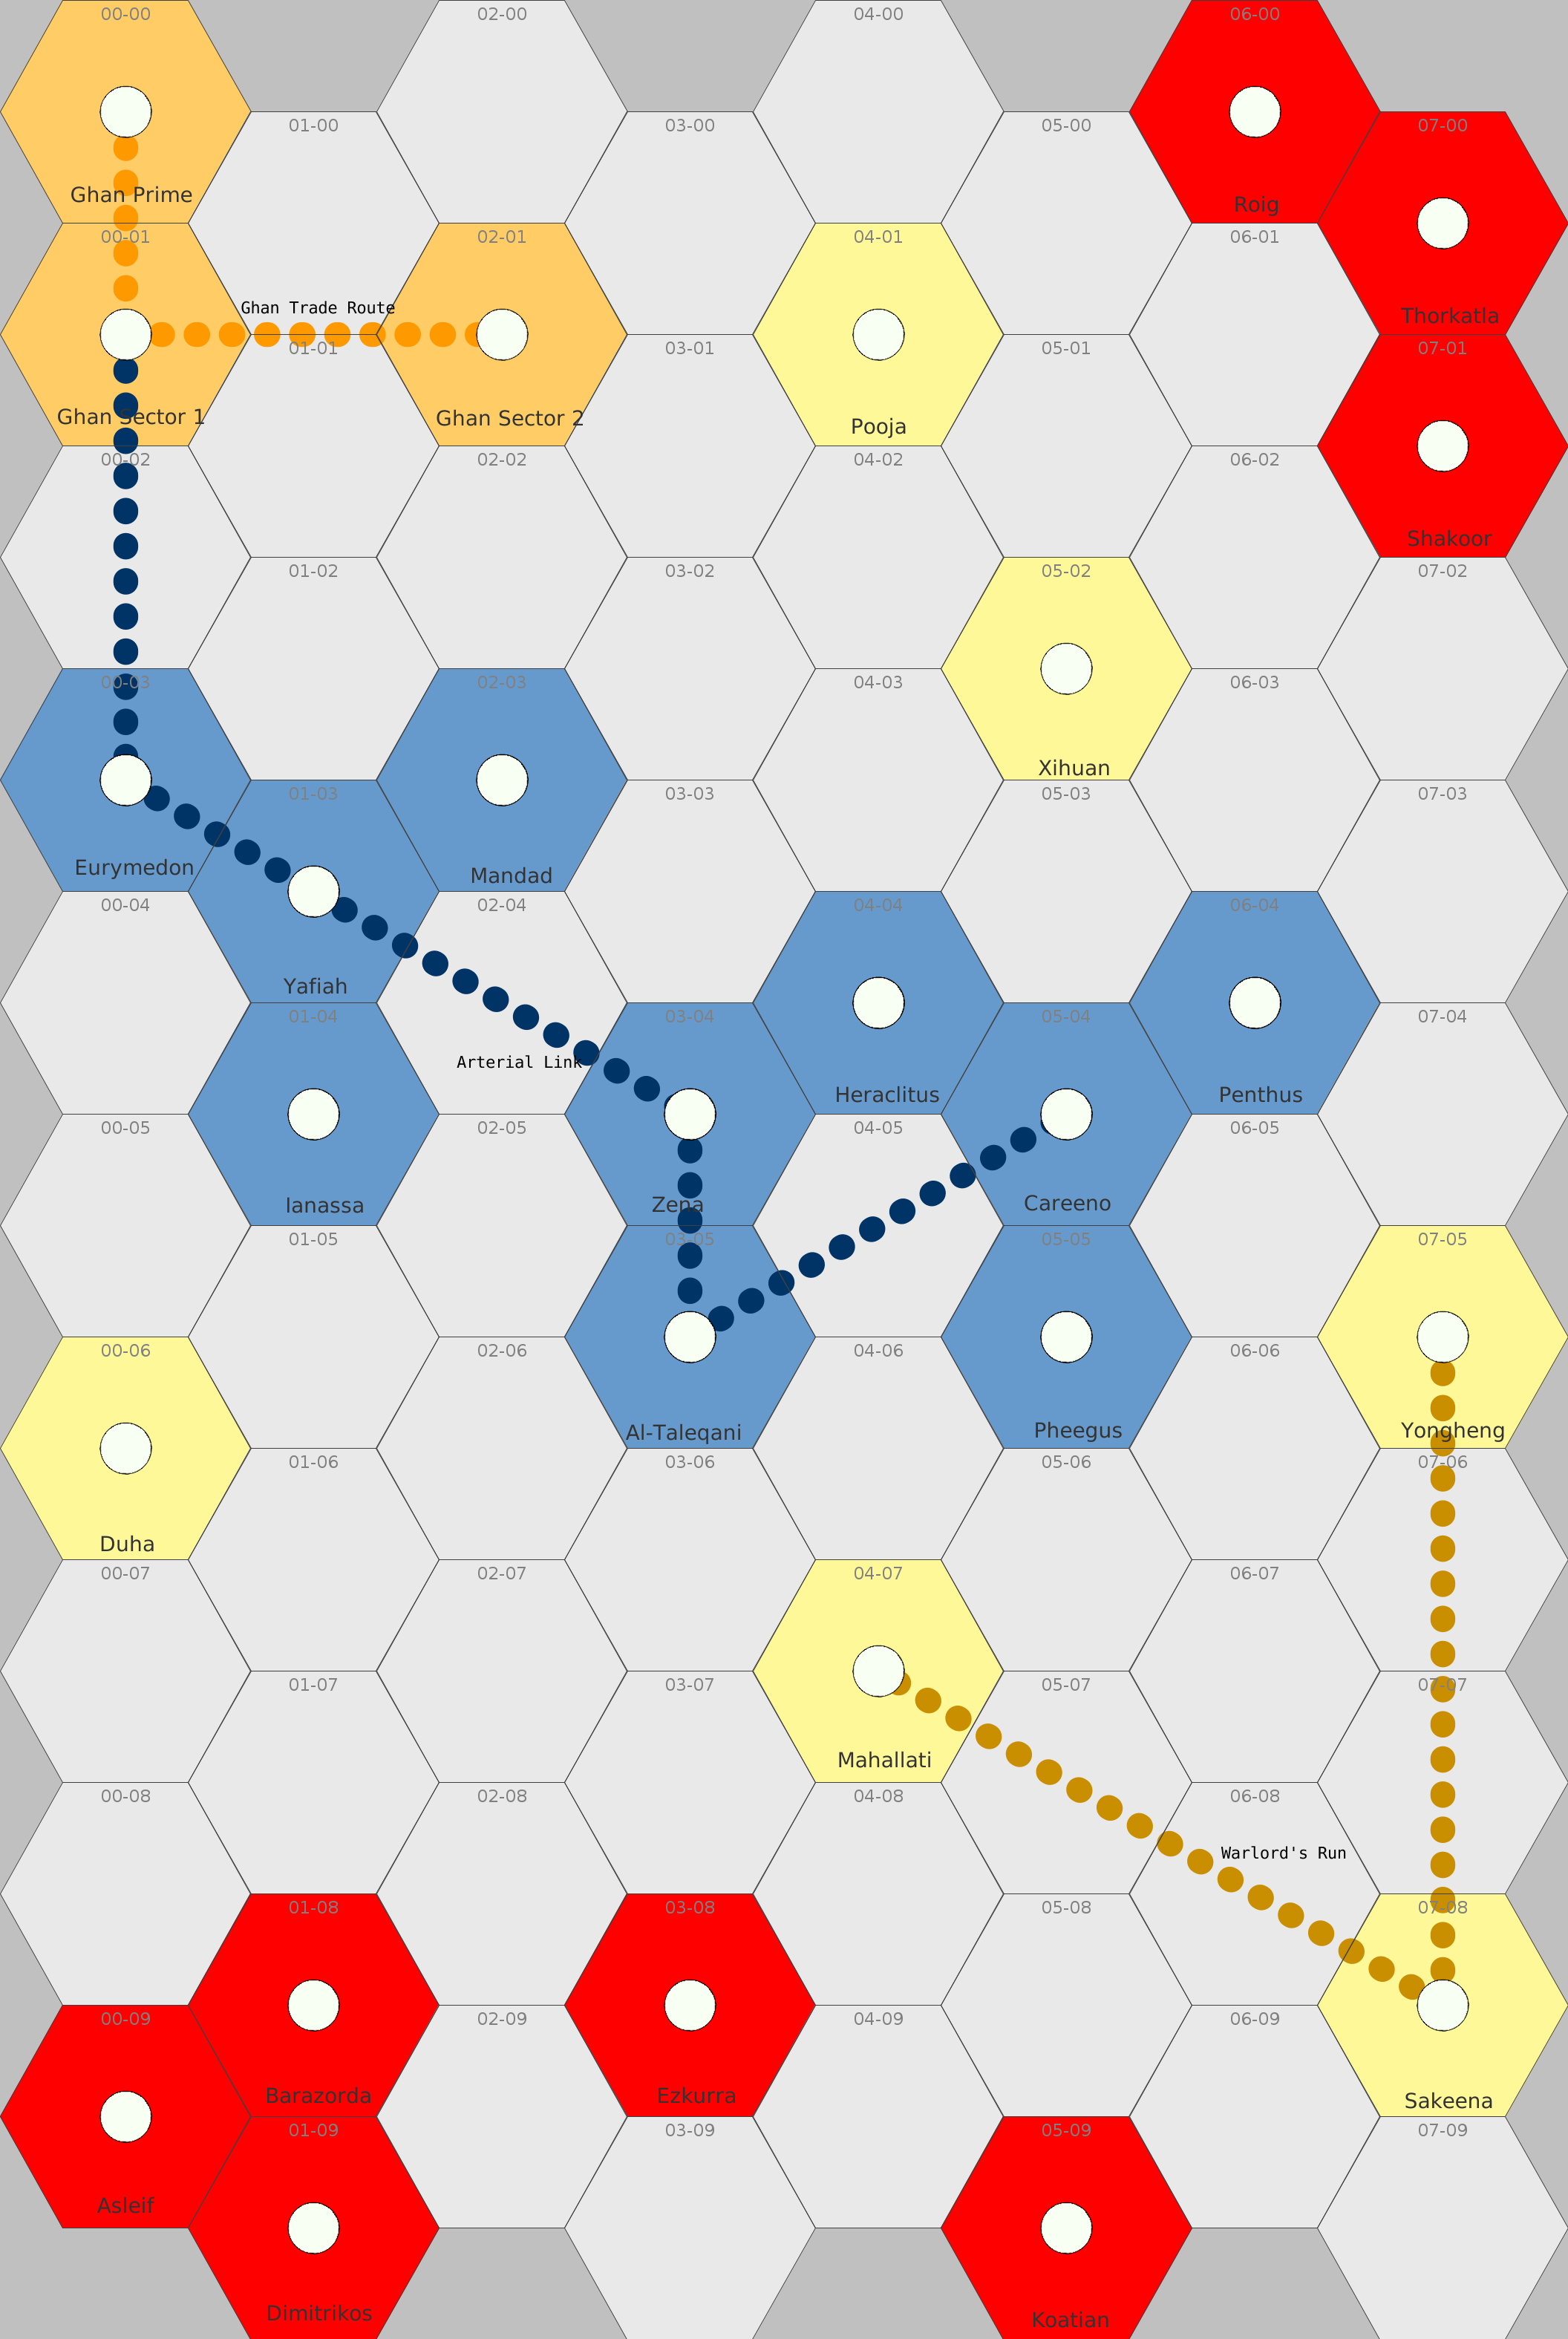
\includegraphics[height=220mm]{sectormap}
\end{center}

\newpage

\begin{multicols}{2}

  \subsection{Sector Overview}

  Sector Shangra Omega consists of 10 \textit{Core} systems (blue), 6 \textit{Independent} systems (yellow), 3 \textit{Ghan} systems (orange) and possibly up to 8 \textit{Lost} systems (red). The systems that surround Shangra Omega are largely unexplored, and Pre-Surge star charts are severely out of date. The sector map used by navigators today are the result of intrepid explorers braving the Black and re-charting the stars.
  
  \begin{redtable}{\linewidth}{bsb}
    \textbf{Name} & \textbf{System} & \textbf{Type}\\
    Al-Taleqani & 03-05 & Core\\
    Asleif & 00-09 & Lost\\
    Barazorda & 01-08 & Lost\\
    Careeno & 05-04 & Core\\
    Dimitrikos & 01-09 & Lost\\
    Duha & 00-06 & Independent\\
    Eurymedon & 00-03 & Core\\
    Ezkurra & 03-00 & Lost\\
    Ghan Prime & 00-00 & Ghan\\
    Ghan Sector 1 & 00-01 & Ghan\\
    Ghan Sector 2 & 02-01 & Ghan\\
    Heraclitus & 04-04 & Core\\
    Ianassa & 01-04 & Core\\
    Koatian & 05-09 & Lost\\
    Mahallati & 04-07 & Independent\\
    Mandad & 02-03 & Core\\
    Penthus & 06-04 & Core\\
    Pheegus & 05-05 & Core\\
    Pooja & 04-01 & Independent\\
    Roig & 06-00 & Lost\\
    Sakeena & 07-08 & Independent\\
    Shakoor & 07-01 & Lost\\
    Thorkatia & 07-00 & Lost\\
    Xihuan & 05-02 & Independent\\
    Yafiah & 01-03 & Core\\
    Yongheng & 07-05 & Independent\\
    Zena & 03-04 & Core\\
  \end{redtable}
  
  \subsection{Core Systems}

  \textbf{The Core} is the name given to the systems that make up the \textbf{United Planets}, a loose federation of star systems that share a common legal framework and similar military structures. Planets, Habitats, Space Stations and Star Systems are allowed to largely govern themselves, but are subject to Universal Decrees voted upon by the United Systems Council. Each star system that has a habitable planet sends 10 Delegates to the Council (regardless of the number of planets, colonies, space stations, or other habitation in that system), and Delegates do not necessarily need to be democratically appointed.
  
  \begin{genericsection}{Al-Taleqani}
  The most populous star system and a cultural force in the known Black. If you want to find something special, odds are that you can find it in Al-sahhah (the main planet, boasting a population of over 1 billion citizens). Despite it's Arabic name, the sector is culturally diverse and boasts the largest population of Ay-Matak in the sector. Many across the Black make their way to Al-Taleqani in the hopes of striking it rich in the mines of Khadim, in a popular Al-Rhul Productions sim-sense experience, or in the hustle and bustle of the streets of Al-sahhah.
  
  The prominent ideology of the system generally focuses on liberty, individual freedoms and the unity and growth of the United Planets.
  \end{genericsection}
  
  \begin{genericsection}{Careeno}
  Commonly known as the "\textit{Blue Collar System}", Careeno is largely known for it's primary industries. In the skies above Raghd are the large space craft manufactories, along the plains of Mahats are the farms that feed billions, and on Polypheme hums the factories that keep our economy going. As the second most populous system in the United Planets (and a industrial powerhouse), Careeno has enough political clout to challenge the powerful Al-Taleqani Delegates in the Council.
  
  The prominent ideology of the system generally focuses on issues that affect the industrial and agricultural working class. This means that the populace strongly leans towards unions, universal health-care and other forms of workplace protections.
  \end{genericsection}
  
  \begin{genericsection}{Eurymedon}
  Eurymedon is the most curious system in United Planets. On the one side is Aerope, known for it's fear of foreigners and outsiders. And on the other side is Olaria, known for being open to almost everyone and every idea. In between the two is Nishtha, an Olarian colony that is really only known for it's intact Pre-Surge ruins that serve as a pilgrimage site for Pre-Surge enthusiasts. Despite the heated arguments and debates between Aerope and Olaria, war has never threatened the system.
  
  Ideology largely depends on the planet. Aerope is largely isolationist, joining the United Planets reluctantly so that they could enjoy the protection and economy of the Federation (however the planetary government is rather lax in enforcing United Planet laws, especially those regarding psionics). Olaria (and Nishtha) embraces virtually everything.
  \end{genericsection}
  
  \begin{genericsection}{Heraclitus}
  Parezi is one of the few habitated airless planets in the Sector, and it is renowned for it's bubble cities that sprawl across it's surface. The system itself is devoted to mining the mineral dense asteroid fields and gas giants. 
  
  Although the system was largely founded by Al-Taleqani entrepreneurs, the working class find a lot in common with the citizens of Careeno. As such, the people are split in their loyalties to these two political powerhouses.
  \end{genericsection}
  
  \begin{genericsection}{Ianassa}
  Ianassa is known around the Black for it's partially intact Pre-Surge archive on Hildegunn. This has led to many Universities, Academies and corporate R\&D departments being established on the planet, devoted to unlocking the secrets of the past. The quarantined planet Androcles is also in the system, locked away because the unstable magnetosphere and severe weather patterns have marooned many space craft on it's barren surface. There are rumours that there is another Pre-Surge archive on Androcles, but that it contains dangerous knowledge that could destroy the Sector.
  
  The ideology of the system largely focuses on knowledge, education and academic merit.
  \end{genericsection}
  
  \begin{genericsection}{Mandad}
  The most heavily regulated and restricted system in the United Planets. Primitive sentient aliens were discovered on Aranzta, leading to the Arantza government to the policy of non-interference and dedicating large reserves for the primitives to inhabit. And on Merlo is one of the last remaining refuges for Psionic schools, and the only one to be found in the United Planets. Because of a latent fear of psionics and the possibility that they will bring about the Surge, Merlo is quarantined and it's Psionics heavily regulated.
  
  On Aranzta, the population see that their non-interference methods follow in the path of Pre-Surge civilizations and see themselves the traditional inheritors of the past. Merlo, on the other hand, wants dramatic government reforms when it comes to the issue of Psionics.
  \end{genericsection}
  
  \begin{genericsection}{Penthus}
  Pethus is the only Christian-ruled system in the sector. Bergthora clung to it's faith after the Surge, although it's teachings are different to classical Catholicism due to theological drift. An on-going problem with pirates from the Shakoor system led to the colonization of Semera, a military output designed to ward off undesirables.
  
  The ideology of the system largely revolves around conservatism, religious ideas and traditional values.
  \end{genericsection}
  
  \begin{genericsection}{Pheegus}
  Pheegus is usually seen as a tourist destination for the citizens of the United Systems. Ballesteros is an ocean planet that boasts huge floating cities filled with assorted activities for visitors to do. It also strictly maintains it's Pre-Surge sea-faring culture in an effort to preserve it's past, although some cynics see the cultural shows and festivals as another way to fleece credits from tourists. Orithyia is also a tourist destination but because it boasts the largest population of Altered Humans. Orithyia is known across the Black for it's "Freak shows".
  \end{genericsection}
  
  \begin{genericsection}{Yafiah}
  A common saying across the Black is "\textit{All Bank Accounts leads to Mecisteus}". The sole planet of the Yafiah system has built a reputation as a financial powerhouse. This is mainly due to it's strong protection and privacy laws, which allows corporations and individuals to safely and securely horde their credits.
  \end{genericsection}
  
  \begin{genericsection}{Zena}
  While Al-Taleqani and Careeno are the superpowers of interstellar politics, Zena is the close third. It's position in the middle of the United Systems' territory has meant that it has become the undisputed Trade Hub. It boasts respectable space-yards in orbit above Marider, while Thurid is known for it's industrial output and trading stations.
  
  It's ideology is varied as the population values it's role as the "arbiter" of interstellar politics, often becoming the deciding vote between the Al-Taleqani and Careeno blocs.
  \end{genericsection}
  
  \subsection{Independent Systems}

  Independent systems are those that choose to remain separate from the United Systems. Some chose not to join because they feel that the strict 10 Delegates per system would unfairly discriminate their large populations. Others stay away because the Decrees do not align with their local laws and customs. And some wish to remain as black market havens. Whatever the reason, Independent systems are considered the "Wild West" of the Black.
  
  \begin{genericsection}{Duha}
  The Duha system was denied entry into the United System due to the violent sectarians threatening civil war on the planet of Garrastazu. The planet is torn by the indecision of how to handle psionics, with one side opting for exiling them and the other arguing for integration. The planet is heavily influenced by their sister planet Amir, which is strongly in the anti-camp after psionic pirates nearly took over the whole planet almost a century ago.
  \end{genericsection}
  
  \begin{genericsection}{Mahallati}
  The inhabitants of Salimah are devoted to the genetic enhancement of the human species. The hope to achieve this by utilizing multiple methods including arranged marriages, cloning, fetal restructuring and post-natal surgery. While they tolerate an alien presence on their planet, only humans enjoy the benefits of full citizenship. Salimah is permanently rejected from the United Systems due to it's use of infanticide to rid it's population of genetic impurities.\\
  On the other spectrum is Vinata, a world full of bubble cities that are under threat due to it's persistent civil war. The war is over a difference of opinion; some wish to become part of the United Systems while others want to embrace the genetic purity of their sister planet Salimah. There are rumours that the civil war is secretly fueled by the Sakeena system so that the Mahallati system does not fall into the United System's sphere of influence.
  \end{genericsection}
  
  \begin{genericsection}{Pooja}
  The desert planet of Dirce is suffering a civil war as warlords fight over the limited water supplies on the planet. The planet itself was largely inhabited by the Ghoa, and is unofficially known as "\textit{Reptile World}". It is not clear whether the civil war started because of limited water supply or because the Ghoa are naturally inclined to fight each other. A "gentleman's agreement" limits the fighting to inside the planet's atmosphere, so visitors are largely safe to dock at the local spaceport and trade is highly sought after.
  \end{genericsection}
  
  \begin{genericsection}{Sakeena}
  Sakeena is a largely self-sufficient star system that strictly follows a protectionist foreign policy. They see the United Systems as a threat to their sovereignty, and actively work to make sure the United Systems do not interfere with their 'sphere of influence'. Many think that the Sakeena system actively encourages the tensions within the Mahallati and Yongheng systems so that they cannot join the United Systems.
  \end{genericsection}
  
  \begin{genericsection}{Xihuan}
  This system is also known as the "\textit{Psionic System}" due to the psionic's school on Ba’albaki and the psionic elite that rule on Thorhalla. It is the only place in the whole Black where psionics are truly free (the only place in the United Systems is the restricted psionic's school in the Mandad system). The system expressly rejects membership to the United Systems, seeing the restrictions on psionic freedoms as barbaric and cruel.
  \end{genericsection}
  
  \begin{genericsection}{Yongheng}
  The planet Vargos in the Yongheng system is embroiled in a decades long civil war. The war originally broke out after the planet Theano was colonized, with six factions claiming ownership. The six factions are: Associated States of Yongheng, Federated States of New Shanghai, South Sodality, Theano Pact, Union of Vargos, and the Vargos Commonality. Vargos itself has been spared the ravages of war as most fighting is done on the surface of Theano, with each faction fighting over patches of territory on the planets surface.
  \end{genericsection}

  \subsection{Ghan Systems}
  
  Ghan systems are, quite simply, the home systems for the Ghantak. Ghan Prime has the homeworld of Ghan, and the Ghantak were able to colonize (at least) two other star systems before the Surge. These systems have all managed to survive the Surge and re-establish contact with each other, but choose to remain separate from the United Systems. They are led by an Empress who resides in Ghan Prime, but each planet is governed by a Hive Queen that has the freedom to do as she pleases.

  \subsection{Lost Systems}
  
  Lost systems are those that are speculated to still exist, but no formal communication or expedition exist to explore them fully. Travel to the Lost systems are fraught with danger, as many do not return.
  
  % Military
  \subsection{Military Ranks}

There will always be a need for a standing military service, and in the Pre-Surge days the powers that be decided on a single rank system for all servicemen (whether army or navy). This standard has been carried on after the Surge, and even warring factions on Independant worlds are known to use the system.

\subsubsection{Enlisted}

Enlisted men provide the manpower for the military services. They serve as the marines, infantry, pilots, engineers, and any other role that is required of them. They can advanced through the ranks in either leadership roles or as specialised experts in their field.

\begin{redtable}{\linewidth}{@{}L{1}@{}}
  \textbf{Private (PVT)}\\
  The lowest rank\\
  \textbf{Specialist (SPC)}\\
  Used to designate an individual with special skills\\
  \textbf{Corporal (CPL)}\\
  Leader of a team (4 servicemen), or Senior specialists or administrative staff\\
  \textbf{Sergeant (SGT)}\\
  Leader of a section (2-3 teams, 8-15 servicemen), or Senior staff for command-level officers\\
  \textbf{Master Sergeant (MSG)}\\
  Highest rank for non-commissioned officers. Senior staff or supervisors of the enlisted men\\
\end{redtable}

\subsubsection{Officers}

Officers provide leadership for the men under their command. They command large numbers of men or military spacecraft, and only rise up the ranks through exemplary service.

\begin{redtable}{\linewidth}{@{}L{1}@{}}
  \textbf{Ensign (ENS)}\\
  Entry-level rank for officers. Generally put in charge of a secion with the aide of a Sergeant\\
  \textbf{Lietenant (LT)}\\
  Leader of a platoon (2-3 sections, 16-45 servicemen), or subordinate for command-level officers\\
  \textbf{Major (MAJ)}\\
  Leader of a company (3-4 platoons, 50-180 servicemen), or commands a small spacecraft\\
  \textbf{Commander (CDR)}\\
  Leader of a battalion (3-4 companies, 200-700), or commands a medium spacecraft\\
  \textbf{Captain (CPT)}\\
  Leader of a brigade (3-4 battalions, 1000-3000), or commands a large spacecraft\\
  \textbf{Colonel (COL)}\\
  Leader of a division (4-5 brigades, 4000-15000), or commands a flotilla (2+ spacecraft)\\
  \textbf{Vice Admiral (VADM)}\\
  Leader of a corps (2-3 divisions, 15000-45000), or commands a group (2+ flotilla). Some infantry forces prefer the older "Lietenant General"\\
  \textbf{Admiral (ADM)}\\
  Leader of an army (2-3 corps, 80000+), or commands a fleet (2+ groups). Some infantry forces prefer the older "General". Seniority is designated by stars, with the highest achievable rank is a 6-star Admiral/General\\
\end{redtable}

\end{multicols}

\newpage

% Worlds
% =================
% Worlds
% =================
\subsection{Worlds}

\begin{multicols}{2}

  \subsubsection{Tech-Levels}
  \label{sec:sector-tech-levels}

  Tech-Levels are a standard way to categorize the differing manufacturing capabilities of a planet. Some worlds are purposely kept at low tech-levels as they provide primary trade resources for high tech-level worlds (such as agriculture).
  
  To see how Gear and Tech-Levels relate to each other, please refer to the \textit{\hyperref[sec:gear-rules]{Gear Tech-Level section}}

  \begin{standardtable}{\linewidth}{ssb}
    \textbf{Level} & \textbf{Description} & \textbf{Example}\\
    0 & Stone & Stone, human power\\
    1 & Ancient & Metals, domestic animals, steam engine\\
    2 & Industrial & Fossil fuels, factories, simple machines\\
    3 & Mechanized & Computers, satellites, 20th century era tech\\
    4 & Interstellar & IDD, energy weapons, cyberware \\
    5 & Advanced & Specialized knowledge in a technological field\\
    6 & Pre-Surge & Psionic tech, TDD, exotic tech\\
  \end{standardtable}

  % ATB Rating
  \subsubsection{ATB classification}
\label{sec:sector-atb}

The \textbf{Atmospheric - Temperature - Biosphere} (ATB) rating is the standard classification system for worlds, planets and other naturally occuring stellar bodies. An ATB gives a general overview about the suitability for habitation, or at the very least an idea of what risks there are in colonising the world. The classification uses 3 letters, one for each of the categories of Atmosphere, Temperature and Biosphere.

\subsubsection{Atmosphere}

\begin{genericsection}{A (Airless)}
  There is little to no atmosphere to speak of. Requires a space suit with a constant supply of oxygen
\end{genericsection}

\begin{genericsection}{B (Breatheable)}
  A mix of gases that is within the breatheable range for organic beings. Since each planet has different mixtures, foriegners are always aware of a "new world stink"
\end{genericsection}

\begin{genericsection}{C (Corrosive)}
  Dangerously hostile atmosphere, even with conventional suits and other protective gear. The atmosphere is extremely toxic, and actively corrodes non-native materials
\end{genericsection}

\begin{genericsection}{G (Inert Gas)}
  Atmosphere consists of gases that are not breatheable by organic beings. The atmosphere is otherwise not hostile or poisonous, but requires a constant source of oxygen
\end{genericsection}

\begin{genericsection}{T (Thick)}
  The atmosphere contains gases that are heavier and thicker than an organic can handle. Organics will require the aid of a filtration mask to breathe the atmosphere. It is considered toxic if an organic decides to breathe the air straight over long periods of time (organics can breathe the air for short periods of time, although their breathing will be laboured)
\end{genericsection}

\begin{genericsection}{X (Toxic)}
  These worlds are much more aggressively hostile than corrosive (C) worlds. These worlds have toxic molecules that are able to bypass suit seals during the corrosion process, meaning that they must be purified at regular intervals, reducing the oxygen supply substantially
\end{genericsection}

\subsubsection{Temperature}

\begin{genericsection}{F (Frozen)}
  Average temperature that is close to absolute zero. Some are so cold that the gases have solidified
\end{genericsection}

\begin{genericsection}{C (Cold)}
  These worlds are uncomfortably cold, but are survivable with suitable heavy clothing
\end{genericsection}

\begin{genericsection}{T (Temperate)}
  These worlds have temperature ranges that are similar to Earth
\end{genericsection}

\begin{genericsection}{W (Warm)}
  These worlds are uncomfortably warm, but are survivable. They are either desert worlds, or have thick, humid jungles
\end{genericsection}

\begin{genericsection}{B (Burning)}
  Average temperatures that is close to boiling. Some are so hot that metals exist in molten form
\end{genericsection}

\begin{genericsection}{V (Varied)}
  These worlds have a wide range of temperatures, either due to unique geological features or varying orbits around their star
\end{genericsection}

\subsubsection{Biosphere}

\begin{genericsection}{R (Remnants)}
  The wreckage and ruins of a dead ecology
\end{genericsection}

\begin{genericsection}{M (Microbial)}
  Non-sentient micro-organisms that can exist in almost all types of environments (such as slimes, bacteria, fungus). They may or may not be dangerous
\end{genericsection}

\begin{genericsection}{Z (None)}
  For some reason or other, life did not evolve on this world
\end{genericsection}

\begin{genericsection}{C (Compatible)}
  Substantial portion of native life is biologically compatible with human nutritional needs
\end{genericsection}

\begin{genericsection}{I (Incompatible)}
  None of the native life is biologically compatible with human nutritional needs. Microbial life could potentially be highly allergenic to humans
\end{genericsection}

\begin{genericsection}{H (Hybrid)}
  The native flora and fauna have been intermixed with imported species from Earth. They may or may not be compatible, but are not otherwise hostile
\end{genericsection}

\begin{genericsection}{E (Engineered)}
  Are either paradise planets that have been carefully sculpted, or living forges that produce foodstuffs and minerals for trade
\end{genericsection}

\end{multicols}

  \subsubsection{Core Worlds}
  \label{sec:sector-worlds}

  \begin{powertable}{ p{.10\textwidth} p{.10\textwidth} p{.05\textwidth} p{.05\textwidth} p{.20\textwidth} p{.35\textwidth} }
    \textbf{Name} & \textbf{A-T-B} & \textbf{Pop.} & \textbf{TL} & \textbf{Sector} & \textbf{Tags}\\
    Aerope	    & T-C-H &	10M+  & 3	& Eurymedon (00-03)   & Bigotry, Fear of Psionics\\
    Al-sahhah   & B-V-C & 1B+   & 4 & Al-Taleqani (03-05) & Specialised Technology, Regional Hegemon\\
    Androcles   & B-T-R & 100K+ & 3 & Ianassa (01-04)     & Freak Geology, Quarantined\\
    Arantza     & T-W-C & 1M+   & 4 & Mandad (02-03)      & Restrictive Laws, Primitive Aliens\\
    Ballesteros & T-T-C & 1M+   & 4 & Pheegus (05-05)     & Rigid Culture, Seagoing cities\\
    Bergthora   & A-T-M & 1M+   & 5 & Penthus (06-04)     & Heavy Industry, Theocracy\\
    Hildegunn   & B-W-C &	100K+	& 4	& Ianassa (01-04)     & Pre-Surge Archive, Intelligence\\
    Khadim	    & T-C-I & 100K+ & 3	& Al-Taleqani (03-05) & Gold Rush, Colonised\\
    Mahats	    & T-T-E &	100K+ &	4 & Careeno (05-04)     & Agriculture, Theocracy\\
    Marider	    & A-T-R & 10M+	& 5	& Zena (03-04)        & Heavy Mining, Major Spaceyard\\
    Mecisteus   & B-T-C & 100M+ & 4 & Yafiah (01-03)      & Banking, Local Specialiaty\\
    Merlo       & B-T-I & 1M+   & 3 & Mandad (02-03)      & Psionic School, Quarantined\\
    Nishtha     &	B-C-C &	100K+	& 4	& Eurymedon (00-03)   & Pre-Surge Ruins, Pilgrimage\\
    Olaria      & G-T-C & 10M+  & 5 & Eurymedon (00-03)   & Pre-Surge Cultists, Xenophiles\\
    Orithyia    & G-T-E &	100K+	& 4	& Pheegus (05-05)     & Altered Humans, Agriculture\\
    Parezi	    & A-W-M & 1M+	  & 4	& Heraclitus (04-04)  & Heavy Mining, Bubble Cities\\
    Polypheme	  & G-V-I & 10M+  &	4 & Careeno (05-04)     &	Trade Hub, Specialised AI\\
    Raghd       & B-T-Z & 1B+   & 5 & Carreno (05-04)     & Flying Cities, Major Spaceyard\\
    Semera      & B-V-I &	100K+	& 4	& Penthus (06-04)     & Outpost, Police State\\
    Thurid      & B-C-C & 100M+ & 4	& Zena (03-04)        & Trade Hub, Heavy Industry\\
  \end{powertable}
 
  \subsubsection{Independent Worlds}

  \begin{powertable}{ p{.10\textwidth} p{.10\textwidth} p{.05\textwidth} p{.05\textwidth} p{.20\textwidth} p{.35\textwidth} }
    \textbf{Name} & \textbf{A-T-B} & \textbf{Pop.} & \textbf{TL} & \textbf{Sector} & \textbf{Tags}\\
    Amir        & B-T-C & 1M+   & 4 & Duha (00-06)      & Oceanic World, Fear of Psionics\\
    Ba'albaki	  & B-C-H &	1M+   &	4	& Xihuan (05-02)    & Psionic School, Psionic Worship\\
    Dirce       & B-V-C & 100K+ & 4 & Pooja (04-01)     & Desert World, Civil War\\
    Garrastazu  & T-T-H & 1M+   & 3 & Duha (00-06)      & Violent Sectarians, Heavy Mining\\
    Georghiou	  & B-T-E & 1M+   &	3 &	Sakeena (07-08)   & Colonised, Agriculture\\
    Oeneus      & G-T-I & 1M+   & 3 & Sakeena (07-08)	  & Colonised, Heavy Industry\\
    Sakeena     & T-T-I & 1B+  & 5 & Sakeena (07-08)   & Major Spaceyard, Police State\\
    Salimah	    & B-T-E & 100K+ &	4	& Mahallati (04-07) & Rigid Culture, Eugenic Cultists\\
    Theano      & B-F-H & 100K+ & 3 & Yongheng (07-05)  & Outpost, Hatred\\
    Thorhalla   & T-V-H & 10M+  & 4 & Xihuan (05-02)    & Tyranny, Bigotry\\
    Vinata      & G-W-C & 1M+   & 4 & Mahallati (04-07) & Civil War, Bubble Cities\\
    Vargos      & T-T-H & 1B+   & 3 & Yongheng (07-05)  & Cold War, Warlords\\
  \end{powertable}

  \subsubsection{Lost Worlds}

  \begin{powertable}{ p{.10\textwidth} p{.10\textwidth} p{.05\textwidth} p{.05\textwidth} p{.20\textwidth} p{.35\textwidth} }
    \textbf{Name} & \textbf{A-T-B} & \textbf{Pop.} & \textbf{TL} & \textbf{Sector} & \textbf{Tags}\\
    Akriti      & A-T-C & ?     & ? & Koatian (05-09)     & Zombies, Out of Contact\\
    Chloe       & B-T-C & 100K+ & 2 & Ezkurra (03-08)     & Minimal Contact, Fear of Tech\\
    Echepolos   & ?-T-M & ?     & ? & Shakoor (07-01)     & Radioactive, Tomb World\\
    Gyda        & B-C-C & 10K+  & 3 & Aslief (00-09)      & Xenophobes, Pre-Surge Archive\\
    Maqsood     & B-C-H & 100K+ & 3 & Dimitrikos (01-09)  & Psionic Worship, Out of Contact\\
    Purva       & B-F-C & 100K+ & 3 & Barazorda (01-08)   & Feral, Pre-Surge Cultists\\
    Pylaimenos  &	A-V-Z & ?     &	? & Thorkatia (07-00)   &	Sealed Menace, Unbreaked AI\\
    Sagari      & B-T-C & 10K+  & 4 & Shakoor (07-01)     & Hostile Space, Badlands World\\
    Xanthippe	  & B-T-H &	1M+   &	4	& Roig (06-00)        & Tyranny, Theocracy\\
  \end{powertable}

  \subsubsection{Ghan Worlds}

  \begin{powertable}{ p{.10\textwidth} p{.10\textwidth} p{.05\textwidth} p{.05\textwidth} p{.20\textwidth} p{.35\textwidth} }
    \textbf{Name} & \textbf{A-T-B} & \textbf{Pop.} & \textbf{TL} & \textbf{Sector} & \textbf{Tags}\\
    Ghalla	& B-W-C &	100K+	& 4	& Ghan Sector 1 (00-01) & Trade Hub, Local Speciality\\
    Ghan    & B-T-C & 1B+  & 5 & Ghan (00-00)          & Banking, Regional Hegemon\\
    Ghatla	& T-W-C &	100K+	& 4	& Ghan (00-00)          & Freak Weather, Agriculture\\
    Gharda  &	B-W-C & 100K+ &	4	& Ghan Sector 2 (02-01) & Oceanic, Major Spaceyard\\
    Ghusha	& A-C-M	& 100K+ &	4	& Ghan Sector 2 (02-01) & Heavy Mining, Freak Geology\\
  \end{powertable}
  
  \subsubsection{Space Stations}

  \begin{powertable}{ p{.10\textwidth} p{.05\textwidth} p{.25\textwidth} p{.45\textwidth} }
    \textbf{Name} & \textbf{Pop.} & \textbf{Sector} & \textbf{Tags}\\
    Central Command &	100K+	& Sector 02-04 & Military, Outpost\\
    Goros Station   & 10K+  & Sector 04-02 & Banking, Trade Hub\\
    Raghd Spaceyard &	50K+	& Careeno (05-04) & Major Spaceyard, Industry\\
    Refuge          & 1K+   & Sector 06-05 & Asylum, Trade Hub\\
  \end{powertable}

% Business groups and factions
% =================
% BUSINESS GROUPS AND FACTIONS
% =================
\subsection{Corporations}

\begin{multicols}{2}

  \subsubsection{Astronautics \& Spacecraft}
  
  These corporations are the leaders in the field for creating the complex systems required for FTL and intra-solar travel, and the spacecraft that use them. They also deal with planetary navigational systems, creating the satellites required for GPS triangulation.
  
  \begin{redtable}{\linewidth}{L{.5}L{.5}}
    \textbf{Name} & \textbf{Headquarters}\\
    Curich Engineering        & Marider, Zena (03-04)\\
    Ferris Spacecraft         & Marider, Zena (03-04)\\
    Ghan Spacecraft           & Gharda, Ghan Sector 2 (02-01)\\
    Mavridou Cooperative      & Raghd, Careeno (05-04)\\
    Quebe-Luxfause Systems    & Marider, Zena (03-04)\\
    Sakeena Shipywards        & Sakeena, Sakeena (07-08)\\
    Solar Spacecraft          & Raghd, Careeno (05-04)\\
    Starlette Industries      & Raghd, Careeno (05-04)\\
  \end{redtable}
  
  \subsubsection{Biotech}
  
  Biotech focuses on using the cutting edge of biological and genetic sciences. These corporations can modify foodstuffs to increase it's viability, genetically enchance organics, and create complex organic machines.
  
  \begin{redtable}{\linewidth}{L{.5}L{.5}}
    \textbf{Name} & \textbf{Headquarters}\\
    Gentik                    & Bergthora, Penthus (06-04)\\
    Interstellar Genetics Inc & Mahats, Careeno (05-04)\\
    Morgath Industries        & Khadim, Al-Taleqani (03-05)\\
    Nazari Cooperative        & Olaria, Eurymedon (00-03)\\
    Orithyia Genetics         & Orithyia, Pheegus (05-05)\\
    Umbrella Coorporation     & Ballestreros, Pheegus (05-05)\\
  \end{redtable}
  
  \subsubsection{Construction \& Manufacturing}
  
  These corporations are leaders in terrestrial and space-borne construction, as well as the industrial factories that manufacture most goods in the Black. They can build space habitats, skyscrapers, and asteroid mining stations.
  
  \begin{redtable}{\linewidth}{L{.5}L{.5}}
    \textbf{Name} & \textbf{Headquarters}\\
    Gorallis Metalworking     & Raghd, Careeno (05-04)\\
    Kroeskin Fabrications     & Thurid, Zena (03-04)\\
    Merr-Sonn Industrial      & Al-sahhah, Al-Taleqani (03-05)\\
    Novaplex                  & Mecisteus, Yafiah (01-03)\\
    Panstellar Zaibatsu       & Bergthora, Penthus (06-04)\\
  \end{redtable}
  
  \subsubsection{Consumer Goods, Entertainment\& Finance}
  
  These corporations target the average consumer with goods, entertainment, finance, and even pharmacueticals.
  
  \begin{redtable}{\linewidth}{L{.5}L{.5}}
    \textbf{Name} & \textbf{Headquarters}\\
    Anistonopoulos Clan       & Mecisteus, Yafiah (01-03)\\
    Al-Rhul Media Productions &	Al-sahhah, Al-Taleqani (03-05)\\
    Buy n Large               & Thurid, Zena (03-04)\\
    Ghan Systems              & Ghalla, Ghan Sector 1 (00-01)\\
    Gringotts                 & Mecisteus, Yafiah (01-03)\\
    Haen Studio               & Olaria, Eurymedon (00-03)\\
    Los Pollos Hermanos       & Al-sahhah, Al-Taleqani (03-05)\\
    Saraphis Pharmacueticals  & Mecisteus, Yafiah (01-03)\\
    Velunza Circle            & Olaria, Eurymedon (00-03)\\
  \end{redtable}
  
  \subsubsection{Cybernetics, Electronics \& Software}
  
  Cyberware is the hottest technology in the Black. These corporations uses the latest in scientific discoveries to fuse the organic with the digital. Some also create the electronics that consumers use in their daily lives.
  
  \begin{redtable}{\linewidth}{L{.5}L{.5}}
    \textbf{Name} & \textbf{Headquarters}\\
    Advanced Ideas Mechanics  & Marider, Zena (03-04)\\
    Altin Alliance            &	Polypheme, Careeno (05-04)\\
    Aperture Science, Inc.    & Thurid, Zena (03-04)\\
    Cyberdyne Systems         & Bergthora, Penthus (06-04)\\
    Gowix Computers           & Hildegunn, Ianassa (01-04)\\
    HoloGraphics Interstellar & Mecisteus, Yafiah (01-03)\\
    Imaharatronics            & Olaria, Eurymedon (00-03)\\
    MicroData Technologies    & Al-sahhah, Al-Taleqani (03-05)\\
    Perzome SoftWEAR          & Olaria, Eurymedon (00-03)\\
    Pied Piper                & Hildegunn, Ianassa (01-04)\\
    Wayne Enterprises         & Thurid, Zena (03-04)\\
  \end{redtable}
  
  \subsubsection{Food}
  
  These corporations are the leaders for producing, packaging and transporting the food across the sector.
  
  \begin{redtable}{\linewidth}{L{.5}L{.5}}
    \textbf{Name} & \textbf{Headquarters}\\
    Aqualis Food Conglomerate & Mahats, Careeno (05-04)\\
    Faraj Fishing             & Amir, Duha (00-06)\\
    Nopoulos Partnership      & Ballesteros, Pheegus (05-05)\\
    SuriTech Foodstuffs       & Orithyia, Pheegus (05-05)\\
    Tatum Farming Collective  & Arantza, Mandad (02-03)\\
  \end{redtable}
  
  \subsubsection{Illegal goods \& Mercenaries}
  
  Many of these "corporations" operate outside United Systems law, but are still semi-legal in some Independant systems. They usually smuggle and sell illicit goods from drugs, illegal AI, and even in people. A few are dedicated mercenaries and strong-men, and can pass off as "Security".
  
  \begin{redtable}{\linewidth}{L{.5}L{.5}}
    \textbf{Name} & \textbf{Headquarters}\\
    Asset Group Solutions     & Al-sahhah, Al-Taleqani (03-05)\\
    Barichello Multistellar   & Semera, Penthus (06-04)\\
    Magnus Syndicate          & Sagari, Shakoor (07-01)\\
    Santhe Security           & Mecisteus, Yafiah (01-03)\\
    Spiker Group              & Dirce, Pooja (04-01)\\
    Zea Outfit	              & Vinata, Mahallati (04-07)\\
  \end{redtable}
  
  \subsubsection{Mining, Energy \& Fuel}
  
  Produces the fuel, mining and energy needs for the population of the Black. Includes businesses or "prospectors" that explore the Black looking for valuable resources to exploit.
  
  \begin{redtable}{\linewidth}{L{.5}L{.5}}
    \textbf{Name} & \textbf{Headquarters}\\
    Bellixan Endeavors        & Khadim, Al-Taleqani (03-05)\\
    Burns Industries          & Raghd, Careeno (05-04)\\
    Colonial Mining           & Parezi, Heraclitus (04-04)\\
    Degan Explorations        & Nishtha, Eurymedon (00-03)\\
    Nexcore Mining Corp       & Marider, Zena (03-04)\\
    Parezi Energy             & Parezi, Heraclitus (04-04)\\
  \end{redtable}
  
  \subsubsection{Weapons}
  
  Makes everything from combat armour to handguns.
  
  \begin{redtable}{\linewidth}{L{.5}L{.5}}
    \textbf{Name} & \textbf{Headquarters}\\
    Al-Astra Association      & Al-sahhah, Al-Taleqani (03-05)\\
    Cafu Systems              & Dirce, Pooja (04-01)\\
    Jayhoon Inc.              & Vinata, Mahallati (04-07)\\
    Stark Industries          & Thurid, Zena (03-04)\\
    Striker                   & Sagari, Shakoor (07-01)\\
    West Wind Outfit          & Vargos, Yongheng (07-05)\\
  \end{redtable}
  
\end{multicols}

% Political groups and factions
% =================
% POLITICAL GROUPS AND FACTIONS
% =================
\subsection{Politics}
  
\subsubsection{United Planet Factions}

\begin{redpowertable}{ p{.20\textwidth} p{.05\textwidth} p{.25\textwidth} p{.4\textwidth} }
  \textbf{Name} & \textbf{Seats} & \textbf{Homeworld} & \textbf{Issues}\\
  Buffalo Party     & 5   & Arantza, Mandad (02-03)         & Culture, Traditionalists, Free Market \\
  Cerulean Guild    & 2   & Mecisteus, Yafiah (01-03)       & Progressives, Government reform, Industrial reform, Free Market\\
  Cobalt Consensus  & 7   & Raghd, Careeno (05-04)          & Industrialists, Welfare, Xenophiles \\
  Democratic Party	& 13  & Thurid, Zena (03-04)            &	Government reform, Foreign Policy, Xenophiles\\
  Freedom Element	  & 1   & Mecisteus, Yafiah (01-03)       &	Elitists, Foreign Policy, Protectionist, Autarky (Self-sufficiency), Xenophobia\\
  Homeland Alliance	& 3   & Ballesteros, Pheegus (05-05)    & Bigotry, Culture, Traditionalists, Protectionists\\
  Iron Front	      & 11  & Parezi, Heraclitus (04-04)      &	Working Class, Protectionist, Poverty, Welfare\\
  Libertarian       & 5   & Mecisteus, Yafiah (01-03)       & Progressive, Individual Rights, Industrial reform, Free Market, Xenophiles\\
  Liberty Combine	  & 15  & Al-sahhah, Al-Taleqani (03-05)  &	Foreign Policy, Free Market, Individual Rights\\
  Fellowship        & 3   & Hildegunn, Ianassa (01-04)      &	Progressives, Socialists, Foriegn Policy, Individual Rights\\
  Popular Banner    & 5   & Aerope, Eurymedon (00-03)       &	Working Class, Bigotry, Immigration, Autarky (self-sufficiency)\\
  Psionic Union	    & 3   & Merlo, Mandad (02-03)           &	Psionics, Communists, Government Reform, Individual Rights\\
  Social Federation & 6   & Raghd, Careeno (05-04) 	        & Culture, Industry\\
  Tyrian Consensus	& 4   &	Bergthora, Penthus (05-04)      & Religion, Tradition\\
  Unified Planets   & 11  & Al-sahhah, Al-Taleqani (03-05)  &	Foriegn Policy, Military\\
  Victory Sodality	& 6   & Semera, Penthus (05-04)         &	Traditionalists, State Industry, Military\\
\end{redpowertable}

\begin{multicols}{2}

\subsubsection{Organised Religions}

\begin{genericsection}{Earth Standard}
Earth Standard is a loose classification for any religious system that can trace it's roots back to Earth. Religious belief is one of the few things people hang on to when trying to survive, and many stubbornly refuse to change. These religious beliefs are usually passed down from close family members or friends. Religions include Buddhism, Christianity, Hinduism, Islam, Jews, and Mormonism.
\end{genericsection}

\begin{genericsection}{Neofundamentalist Ideologists}
\textbf{No universal leadership}\\
Born in the classical philosphical teachings of Earth (especially Stoicism). NFI adherants believe in accepting your lot in life, actively resisting temptation, and using Science to further our understanding of the world
\end{genericsection}

\begin{genericsection}{New Catholics}
\textbf{Ruling Council on Bergthora, Penthus}\\
Cut off from the Vatican (and Earth), the primarily Catholic colony at Bergthora created their own Council of Cardinals to provide leadership for their faithful. The Council gradually took over the governance of the entire system. New Catholics are the largest Christian organisation in the sector, mainly because they accept differing ideas on the nature of God and were able to adopt practices of other Christians
\end{genericsection}

\begin{genericsection}{Quietist Muslims}
\textbf{Communal Democracy}\\
Largely concentrated on Mahats in the Careeno system. After the turbulent 21st Century, the Islamic faith began to reject the old power structures and began to democratically guide their faith in the best interests of the community. The faith largely shuns foriegn policy issues that do not affect their world, and strives to limit their involvement with the affairs of nonbelievers. They prefer to keep to their own kind and avoid positions of wealth and power
\end{genericsection}

\begin{genericsection}{Stellarist Muslims}
\textbf{Communal Democracy}\\
Largely concentrated on Mahats in the Careeno system. A reaction to the Quietist movement, Stellarists believe that the movement has drifted too far from the original teachings. Stellarists desire to reintegrate the Islam faith within the larger interstellar community, and allow their members to actively seek positions of power and wealth
\end{genericsection}

\begin{genericsection}{Syncretism}
\textbf{No universal leadership}\\
After the Surge, many colonies began to focus on survival instead of religious fundamentals. This has resulted in many planets mixing and matching tenets from a wide spectrum of beliefs. This is the most common religion found within the sector
\end{genericsection}

\end{multicols}


  % Templates
  \section{Templates}
\label{sec:templates}

\begin{multicols}{2}
%
% New Spacecraft
%
  \subsection{New Spacecraft}
  \label{sec:template-spacecraft}
  
  \subsubsection{Fighters}
  \label{sec:template-fighters}
  
  \textbf{Osa T-1}
  \begin{standardtable}{\linewidth}{sb}
    \textbf{Make}       & Sakeena Shipyards\\
    \textbf{Hull}       & Fighter\\ % Base Cost = 100k
    \textbf{Rank}       & Novice\\ 
    \textbf{Wounds}     & 1\\
    \textbf{Armour}     & d4\\ % 50k
    \textbf{Engines}    & d4\\ % 50k
    \textbf{Power}      & d8\\ % 150k
    \textbf{Bulk}       & d6\\ % 100k
    \textbf{Systems}    & d8\\ % 200k
    \textbf{Skills}     & ECM d8; Navigation d6; Sensors d6; Weapons d8\\
    \textbf{Crew}       & 1\\ % Base = 1
    \textbf{Storage}    & 5\\ % Base = 3 + 1.5
    \textbf{Power}      & 7\\ % Base = 5 + 1.5
    \textbf{Size}       & -1\\
    \textbf{Acc / TS}   & 50 / 700\\ % Base = 50/700
    \textbf{Evade}      & 2\\
    \textbf{Toughness}  & 3\\
    \textbf{Value}      & 550K\\
    \textbf{Maintenance} & 2.75K\\
  \end{standardtable}
  
  \textbf{Kestrel}
  \begin{standardtable}{\linewidth}{sb}
    \textbf{Make}       & Solar Spacecraft\\
    \textbf{Hull}       & Fighter\\ % Base Cost = 100k
    \textbf{Rank}       & Novice\\
    \textbf{Wounds}     & 1\\
    \textbf{Armour}     & d8\\ % Base = 150k
    \textbf{Engines}    & d6\\ % Base = 100k
    \textbf{Power}      & d4\\ % Base = 50k
    \textbf{Bulk}       & d4\\ % Base = 50k
    \textbf{Systems}    & d6\\ % Base = 150k
    \textbf{Skills}     & ECM d8; Navigation d6; Weapons d8\\
    \textbf{Crew}       & 1\\ % Base = 1
    \textbf{Storage}    & 3\\ % Base = 3
    \textbf{Power}      & 3\\ % Base = 5 - 2.5
    \textbf{Size}       & -1\\
    \textbf{Acc / TS}   & 50 / 700\\ % Base = 50/700
    \textbf{Evade}      & 2\\
    \textbf{Toughness}  & 5\\
    \textbf{Value}      & 500K\\
    \textbf{Maintenance} & 2.5K\\
  \end{standardtable}
  
  \textbf{Shaytan}
  \begin{standardtable}{\linewidth}{sb}
    \textbf{Make}       & Starlette Industries\\
    \textbf{Hull}       & Fighter\\ % Base Cost = 100k
    \textbf{Rank}       & Seasoned\\
    \textbf{Wounds}     & 1\\
    \textbf{Armour}     & d10\\ % Base = 200k
    \textbf{Engines}    & d6\\ % Base = 100k
    \textbf{Power}      & d6\\ % Base = 100k
    \textbf{Bulk}       & d4\\ % Base = 50k
    \textbf{Systems}    & d8\\ % Base = 200k
    \textbf{Skills}     & ECM d8; Navigation d8; Sensors d8; Weapons d8\\
    \textbf{Crew}       & 1\\ % Base = 1
    \textbf{Storage}    & 3\\ % Base = 3
    \textbf{Power}      & 5\\ % Base = 5
    \textbf{Size}       & -1\\
    \textbf{Acc / TS}   & 50 / 700\\ % Base = 50/700
    \textbf{Evade}      & 2\\
    \textbf{Toughness}  & 6\\
    \textbf{Value}      & 650K\\
    \textbf{Maintenance} & 3.25K\\
  \end{standardtable}
  
  \subsubsection{Shuttles}
  \label{sec:templates-shuttles}
  
  \textbf{Shangren Yi}
  \begin{standardtable}{\linewidth}{sb}
    \textbf{Make}       & Starlette Industries\\
    \textbf{Hull}       & Shuttle\\ % Base = 250K
    \textbf{Rank}       & Novice\\ 
    \textbf{Wounds}     & 2\\
    \textbf{Armour}     & d4\\ % 125k
    \textbf{Engines}    & d6\\ % 250k
    \textbf{Power}      & d6\\ % 250k
    \textbf{Bulk}       & d8\\ % 375k
    \textbf{Systems}    & d6\\ % 375k
    \textbf{Skills}     & Auto-pilot d6; Navigation d6; Operations d6; Repair d6; Sensors d6 \\
    \textbf{Crew}       & 4\\ % Base = 4
    \textbf{Storage}    & 20\\ % Base = 10
    \textbf{Power}      & 5\\ % Base = 5
    \textbf{Size}       & 0\\
    \textbf{Acc / TS}   & 40 / 600\\ % Base = 40 / 600
    \textbf{Evade}      & 5\\
    \textbf{Toughness}  & 4\\
    \textbf{Value}      & 1.375M\\
    \textbf{Maintenance} & 6.88K\\
  \end{standardtable}
  
  \subsubsection{Patrol}
  \label{sec:templates-patrol}
  
  \textbf{Kibo FFS}
  \begin{standardtable}{\linewidth}{sb}
    \textbf{Make}       & Sakeena Shipyards\\
    \textbf{Hull}       & Patrol\\ % Base = 250K
    \textbf{Rank}       & Novice\\
    \textbf{Wounds}     & 2\\
    \textbf{Armour}     & d4\\ % 125k
    \textbf{Engines}    & d8\\ % 375k
    \textbf{Power}      & d6\\ % 250k
    \textbf{Bulk}       & d8\\ % 375k
    \textbf{Systems}    & d4\\ % 250k
    \textbf{Skills}     & Auto-pilot d6; Navigation d6; Operations d4; Sensors d6\\
    \textbf{Crew}       & 4\\ % Base = 4
    \textbf{Storage}    & 10\\ % Base = 5
    \textbf{Power}      & 10\\ % Base = 10
    \textbf{Size}       & 0\\
    \textbf{Acc / TS}   & 45 / 600\\ % Base = 45/600
    \textbf{Evade}      & 5\\
    \textbf{Toughness}  & 4\\
    \textbf{Value}      & 1.375M\\
    \textbf{Maintenance} & 6.88K\\
  \end{standardtable}
  
  \subsubsection{Corvette}
  \label{sec:templates-corvette}
  
  \textbf{Falcon}
  \begin{standardtable}{\linewidth}{sb}
    \textbf{Make}       & Solar Spacecraft\\
    \textbf{Hull}       & Corvette\\
    \textbf{Rank}       & Novice\\ % Base = 500k
    \textbf{Wounds}     & 3\\
    \textbf{Armour}     & d6\\ % 500k
    \textbf{Engines}    & d8\\ % 750k
    \textbf{Power}      & d6\\ % 500k
    \textbf{Bulk}       & d4\\ % 250k
    \textbf{Systems}    & d6\\ % 750k
    \textbf{Skills}     & Navigation d6; Operations d6; Sensors d8; Weapons d6\\
    \textbf{Crew}       & 10\\ % Base = 10
    \textbf{Storage}    & 20\\ % Base = 20
    \textbf{Power}      & 15\\ % Base = 15
    \textbf{Size}       & +1\\
    \textbf{Acc / TS}   & 35 / 400\\ % Base = 35/400
    \textbf{Evade}      & 2\\
    \textbf{Toughness}  & 6\\
    \textbf{Value}      & 2.75M\\
    \textbf{Maintenance} & 13.75K\\
  \end{standardtable}
  
  \textbf{Hawk}
  \begin{standardtable}{\linewidth}{sb}
    \textbf{Make}       & Solar Spacecraft\\
    \textbf{Hull}       & Corvette\\
    \textbf{Rank}       & Seasoned\\ % Base = 500k
    \textbf{Wounds}     & 3\\
    \textbf{Armour}     & d6\\ % 500k
    \textbf{Engines}    & d10\\ % 1M
    \textbf{Power}      & d6\\ % 500k
    \textbf{Bulk}       & d8\\ % 750k
    \textbf{Systems}    & d8\\ % 1M
    \textbf{Skills}     & Auto-pilot d6; Navigation d8; Operations d4; Sensors d6; Weapons d6\\
    \textbf{Crew}       & 10\\ % Base = 10
    \textbf{Storage}    & 40\\ % Base = 20
    \textbf{Power}      & 15\\ % Base = 15
    \textbf{Size}       & +1\\
    \textbf{Acc / TS}   & 53 / 600\\ % Base = 35/400
    \textbf{Evade}      & 5\\
    \textbf{Toughness}  & 6\\
    \textbf{Value}      & 3.75M\\
    \textbf{Maintenance} & 18.75K\\
  \end{standardtable}
%
% Characters
%
  \subsection{New Characters}
  \label{sec:templates-characters}
  
  \subsubsection{Ghoa}
  \label{sec:templates-ghoa}
  
  \textbf{Ghoan Warrior}
  \begin{standardtable}{\linewidth}{sb}
    \textbf{Rank}       & Novice\\
    \textbf{Strength}   & d8\\
    \textbf{Agility}    & d8\\
    \textbf{Smarts}     & d4\\
    \textbf{Spirit}     & d4\\
    \textbf{Vigor}      & d8\\
    \textbf{Skills}     & Fighting d10; Shooting d10; Intimidation d8\\
    \textbf{Charisma}   & -4\\
    \textbf{Pace}       & 6\\
    \textbf{Parry}      & 7\\
    \textbf{Toughness}  & 6\\
    \textbf{Bloodthirsty} & -2 Charisma (included)\\
    \textbf{Natural Weapons} & Claws, Teeth and Tail does STR+d6\\
    \textbf{Reptile Blood} & -4 to resist cold\\
    \textbf{Stronger} & Start with a d6 in STR (included)\\
    \textbf{Free Edge} & Start with one free Novice Edge\\
  \end{standardtable}
  
  \subsubsection{Uplifted}
  \label{sec:templates-uplifted}
  
  \textbf{Bear Pirate}
  \begin{standardtable}{\linewidth}{sb}
    \textbf{Rank}       & Novice\\
    \textbf{Strength}   & d6\\
    \textbf{Agility}    & d8\\
    \textbf{Smarts}     & d4\\
    \textbf{Spirit}     & d4\\
    \textbf{Vigor}      & d8\\
    \textbf{Skills}     & Fighting d10; Shooting d10; Intimidation d8\\
    \textbf{Charisma}   & -4\\
    \textbf{Pace}       & 5\\
    \textbf{Parry}      & 7\\
    \textbf{Toughness}  & 9\\
    \textbf{Inferior} & -2 Charisma (included) \\
    \textbf{Primal Weapons} & Claws / Teeth does STR+d6 damage\\
    \textbf{Primitive Intellect} & -1 to Smarts-based checks\\
    \textbf{Bear Ancestry} & +1 Size, +3 Toughness (included)\\
    \textbf{Free Edge} & Start with one free Novice Edge\\
  \end{standardtable}
  
  \textbf{Ferret Infiltrator}
  \begin{standardtable}{\linewidth}{sb}
    \textbf{Rank}       & Novice\\
    \textbf{Strength}   & d4\\
    \textbf{Agility}    & d8\\
    \textbf{Smarts}     & d6\\
    \textbf{Spirit}     & d6\\
    \textbf{Vigor}      & d6\\
    \textbf{Skills}     & Shooting d8; Stealth d8; Survival d8\\
    \textbf{Charisma}   & -3\\
    \textbf{Pace}       & 8\\
    \textbf{Parry}      & 2\\
    \textbf{Toughness}  & 5\\
    \textbf{Inferior} & -2 Charisma (included) \\
    \textbf{Primal Weapons} & Claws / Teeth does STR+d6 damage\\
    \textbf{Primitive Intellect} & -1 to Smarts-based checks\\
    \textbf{Rodent Ancestry} & +4 Pace (included)\\
    \textbf{Free Edge} & Start with one free Novice Edge\\
  \end{standardtable}
  
  \textbf{Rabbit Cyberware Trader}
  \begin{standardtable}{\linewidth}{sb}
    \textbf{Rank}       & Novice\\
    \textbf{Strength}   & d4\\
    \textbf{Agility}    & d4\\
    \textbf{Smarts}     & d8\\
    \textbf{Spirit}     & d10\\
    \textbf{Vigor}      & d4\\
    \textbf{Skills}     & Computers d8; Persuasion d10; Repair d8\\
    \textbf{Charisma}   & -1\\
    \textbf{Pace}       & 8\\
    \textbf{Parry}      & 2\\
    \textbf{Toughness}  & 4\\
    \textbf{Inferior} & -2 Charisma (included) \\
    \textbf{Primal Weapons} & Claws / Teeth does STR+d6 damage\\
    \textbf{Primitive Intellect} & -1 to Smarts-based checks\\
    \textbf{Rodent Ancestry} & +4 Pace (included)\\
    \textbf{Free Edge} & Start with one free Novice Edge\\
  \end{standardtable}
  
\end{multicols}

  % Templates
  \section{Character Sheet}

\begin{multicols}{2}

  \textbf{Personal Details}
  
  \begin{redtable}{\linewidth}{@{}L{.25}@{}L{.75}@{}}
    \textbf{Name} & \uline{ \hfill} \\
    \textbf{Species} & \uline{ \hfill} \\
    \textbf{Career} & \uline{ \hfill} \\
    \textbf{Homeworld} & \uline{ \hfill} \\
    \textbf{Age} & \uline{ \hfill} \\
    \textbf{Height} & \uline{ \hfill} \\
    \textbf{Weight} & \uline{ \hfill} \\
    \textbf{Gender} & \uline{ \hfill} \\
    \textbf{Rank} & \uline{ \hfill} \\
    \textbf{XP} & \uline{ \hfill}
  \end{redtable}
  
  \hline

  \textbf{Attributes}
  \begin{redtable}{\linewidth}{@{}L{0.35}@{}C{0.65}@{}}
    \textbf{Agility} & $\bigcirc$ d4/$\bigcirc$ d6/$\bigcirc$ d8/$\bigcirc$ d10/$\bigcirc$ d12\\
    \textbf{Smarts} & $\bigcirc$ d4/$\bigcirc$ d6/$\bigcirc$ d8/$\bigcirc$ d10/$\bigcirc$ d12\\
    \textbf{Spirit} & $\bigcirc$ d4/$\bigcirc$ d6/$\bigcirc$ d8/$\bigcirc$ d10/$\bigcirc$ d12\\
    \textbf{Strength} & $\bigcirc$ d4/$\bigcirc$ d6/$\bigcirc$ d8/$\bigcirc$ d10/$\bigcirc$ d12\\
    \textbf{Vigor} & $\bigcirc$ d4/$\bigcirc$ d6/$\bigcirc$ d8/$\bigcirc$ d10/$\bigcirc$ d12
  \end{redtable}
  
  \hline
  
  \textbf{Skills}
  \begin{redtable}{\linewidth}{@{}L{0.35}@{}C{0.65}@{}}
     \uline{\hfill} & $\bigcirc$ d4/$\bigcirc$ d6/$\bigcirc$ d8/$\bigcirc$ d10/$\bigcirc$ d12\\
     \uline{\hfill} & $\bigcirc$ d4/$\bigcirc$ d6/$\bigcirc$ d8/$\bigcirc$ d10/$\bigcirc$ d12\\
     \uline{\hfill} & $\bigcirc$ d4/$\bigcirc$ d6/$\bigcirc$ d8/$\bigcirc$ d10/$\bigcirc$ d12\\
     \uline{\hfill} & $\bigcirc$ d4/$\bigcirc$ d6/$\bigcirc$ d8/$\bigcirc$ d10/$\bigcirc$ d12\\
     \uline{\hfill} & $\bigcirc$ d4/$\bigcirc$ d6/$\bigcirc$ d8/$\bigcirc$ d10/$\bigcirc$ d12\\
     \uline{\hfill} & $\bigcirc$ d4/$\bigcirc$ d6/$\bigcirc$ d8/$\bigcirc$ d10/$\bigcirc$ d12\\
     \uline{\hfill} & $\bigcirc$ d4/$\bigcirc$ d6/$\bigcirc$ d8/$\bigcirc$ d10/$\bigcirc$ d12\\
     \uline{\hfill} & $\bigcirc$ d4/$\bigcirc$ d6/$\bigcirc$ d8/$\bigcirc$ d10/$\bigcirc$ d12\\
     \uline{\hfill} & $\bigcirc$ d4/$\bigcirc$ d6/$\bigcirc$ d8/$\bigcirc$ d10/$\bigcirc$ d12\\
     \uline{\hfill} & $\bigcirc$ d4/$\bigcirc$ d6/$\bigcirc$ d8/$\bigcirc$ d10/$\bigcirc$ d12\\
     \uline{\hfill} & $\bigcirc$ d4/$\bigcirc$ d6/$\bigcirc$ d8/$\bigcirc$ d10/$\bigcirc$ d12
  \end{redtable}
  
  \hline
  
  \textbf{Derived Stats}
  \begin{redtable}{\linewidth}{@{}L{0.65}@{}L{0.15}@{}L{0.2}@{}}
     \textbf{Statistic} & \textbf{Base} & \textbf{Mod}\\
     Carry Load \textit{$( 3 \times Strength)$} kg & \uline{\hfill} & \uline{\hfill} \\
     Charisma \textit{$( (Spirit \div 2) - 4 )$} & \uline{\hfill} & \uline{\hfill} \\
     Pace \textit{$( (Strength \div 2) + 2 )$} & \uline{\hfill} & \uline{\hfill} \\
     Parry \textit{$( (Fighting \div 2) + 2 )$}  & \uline{\hfill} & \uline{\hfill} \\
     Toughness \textit{$( (Vigor \div 2) + 2 )$}  & \uline{\hfill} & \uline{\hfill} 
  \end{redtable}
  
  \hline
  
  \textbf{Credits}
  \begin{redtable}{\linewidth}{@{}L{0.6}@{}L{0.4}@{}}
     Cash \textit{(On person or card)} & \uline{\hfill} \\
     Deposit \textit{(Include name of bank)} & \uline{\hfill} \\
     Debt \textit{(Include name of debtor/s)} & \uline{\hfill} 
  \end{redtable}
  
  \hline
  
  \textbf{Contacts}
  \begin{redtable}{\linewidth}{@{}L{0.4}@{}L{0.4}@{}L{0.2}@{}}
    \textbf{Name} & \textbf{Type} & \textbf{Location} \\
    \uline{\hfill} & \uline{\hfill} & \uline{\hfill} \\
    \uline{\hfill} & \uline{\hfill} & \uline{\hfill} \\
    \uline{\hfill} & \uline{\hfill} & \uline{\hfill} \\
    \uline{\hfill} & \uline{\hfill} & \uline{\hfill} \\
    \uline{\hfill} & \uline{\hfill} & \uline{\hfill} 
  \end{redtable}
  
  \hline
  
  \textbf{Gear}
  
  \uline{\hfill}
  
  \uline{\hfill}
  
  \uline{\hfill}
  
  \uline{\hfill}
  
  \uline{\hfill}
  
  \uline{\hfill}
  
  \uline{\hfill}
  
  \uline{\hfill}
  
  \uline{\hfill}
  
  \uline{\hfill}
  
  \uline{\hfill}
  
  \uline{\hfill}
  
  \uline{\hfill}
  
  \hline
  
  \textbf{Armour}

  \begin{redtable}{\linewidth}{@{}L{0.3}@{}L{0.2}@{}L{0.2}@{}L{0.2}@{}}
    \textbf{Name} & \textbf{Area} & \textbf{Prot.} & \textbf{Wgt.}\\
    \uline{\hfill} & \uline{\hfill} & \uline{\hfill} & \uline{\hfill} \\
    \uline{\hfill} & \uline{\hfill} & \uline{\hfill} & \uline{\hfill} \\
    \uline{\hfill} & \uline{\hfill} & \uline{\hfill} & \uline{\hfill} 
  \end{redtable}
  
\end{multicols}

\textbf{Weapon}

\begin{redtable}{\linewidth}{@{}L{.20}@{}L{.10}@{}L{.10}@{}L{.10}@{}L{.50}@{}}
  \textbf{Name} & \textbf{Range} & \textbf{RoF} & \textbf{Damage} & \textbf{Notes}\\
  \uline{\hfill} & \uline{\hfill} & \uline{\hfill} & \uline{\hfill} & \uline{\hfill} \\
  \uline{\hfill} & \uline{\hfill} & \uline{\hfill} & \uline{\hfill} & \uline{\hfill} \\
  \uline{\hfill} & \uline{\hfill} & \uline{\hfill} & \uline{\hfill} & \uline{\hfill} \\
  \uline{\hfill} & \uline{\hfill} & \uline{\hfill} & \uline{\hfill} & \uline{\hfill} 
\end{redtable}

\hline

\textbf{Shaken:} $\bigcirc$ / \textbf{Wounds:} $\bigcirc$ $\bigcirc$ $\bigcirc$ / \textbf{Fatigue:} $\bigcirc$ $\bigcirc$ / \textbf{Effects:} \uline{\hfill} 

\newpage

\textbf{Hindrances}
  
\begin{redtable}{\linewidth}{@{}L{0.3}@{}L{0.7}@{}}
   \textbf{Name} & \textbf{Detail} \\
   \uline{\hfill} & \uline{\hfill} \\
   \uline{\hfill} & \uline{\hfill} \\
   \uline{\hfill} & \uline{\hfill} \\
   \uline{\hfill} & \uline{\hfill} 
\end{redtable}
  
\hline

\textbf{Edges}
  
\begin{redtable}{\linewidth}{@{}L{0.3}@{}L{0.7}@{}}
   \textbf{Name} & \textbf{Detail} \\
   \uline{\hfill} & \uline{\hfill} \\
   \uline{\hfill} & \uline{\hfill} \\
   \uline{\hfill} & \uline{\hfill} \\
   \uline{\hfill} & \uline{\hfill} \\
   \uline{\hfill} & \uline{\hfill} \\
   \uline{\hfill} & \uline{\hfill} \\
   \uline{\hfill} & \uline{\hfill} \\
   \uline{\hfill} & \uline{\hfill} \\
   \uline{\hfill} & \uline{\hfill} \\
   \uline{\hfill} & \uline{\hfill} 
\end{redtable}

\hline

\textbf{Cyberware}

\begin{redtable}{\linewidth}{@{}L{.20}@{}L{.10}@{}L{.10}@{}L{.10}@{}@{}L{.10}L{.40}@{}}
  \textbf{Name} & \textbf{Skill} & \textbf{Charge} & \textbf{Range} & \textbf{Time} & \textbf{Effect}\\
  \uline{\hfill} & \uline{\hfill} & \uline{\hfill} & \uline{\hfill} & \uline{\hfill} & \uline{\hfill} \\
  \uline{\hfill} & \uline{\hfill} & \uline{\hfill} & \uline{\hfill} & \uline{\hfill} & \uline{\hfill} \\
  \uline{\hfill} & \uline{\hfill} & \uline{\hfill} & \uline{\hfill} & \uline{\hfill} & \uline{\hfill} \\
  \uline{\hfill} & \uline{\hfill} & \uline{\hfill} & \uline{\hfill} & \uline{\hfill} & \uline{\hfill} \\
  \uline{\hfill} & \uline{\hfill} & \uline{\hfill} & \uline{\hfill} & \uline{\hfill} & \uline{\hfill} \\
  \uline{\hfill} & \uline{\hfill} & \uline{\hfill} & \uline{\hfill} & \uline{\hfill} & \uline{\hfill} 
\end{redtable}

\textit{Cyberware Programs}

\uline{\hfill}

\hline

\textbf{Psionics}

\begin{redtable}{\linewidth}{@{}L{.20}@{}L{.10}@{}L{.10}@{}@{}L{.10}L{.50}@{}}
  \textbf{Name} & \textbf{Penalty} & \textbf{Range} & \textbf{Time} & \textbf{Effect}\\
  \uline{\hfill} & \uline{\hfill} & \uline{\hfill} & \uline{\hfill} & \uline{\hfill} \\
  \uline{\hfill} & \uline{\hfill} & \uline{\hfill} & \uline{\hfill} & \uline{\hfill} \\
  \uline{\hfill} & \uline{\hfill} & \uline{\hfill} & \uline{\hfill} & \uline{\hfill} \\
  \uline{\hfill} & \uline{\hfill} & \uline{\hfill} & \uline{\hfill} & \uline{\hfill} \\
  \uline{\hfill} & \uline{\hfill} & \uline{\hfill} & \uline{\hfill} & \uline{\hfill} \\
  \uline{\hfill} & \uline{\hfill} & \uline{\hfill} & \uline{\hfill} & \uline{\hfill} \\
  \uline{\hfill} & \uline{\hfill} & \uline{\hfill} & \uline{\hfill} & \uline{\hfill} \\
  \uline{\hfill} & \uline{\hfill} & \uline{\hfill} & \uline{\hfill} & \uline{\hfill} 
\end{redtable}

\hline

\textbf{Background}

\uline{\hfill}

\uline{\hfill}

\uline{\hfill}

\uline{\hfill}

\uline{\hfill}

\uline{\hfill}

  \section{Spacecraft Sheet}

\begin{multicols}{2}

  \textbf{Details}
  
  \begin{redtable}{\linewidth}{@{}L{.25}@{}L{.75}@{}}
    \textbf{Name} & \uline{ \hfill} \\
    \textbf{Type} & \uline{ \hfill} \\
    \textbf{Make} & \uline{ \hfill} \\
    \textbf{Model} & \uline{ \hfill} \\
    \textbf{Age} & \uline{ \hfill} \\
    \textbf{Rank} & \uline{ \hfill} \\
    \textbf{XP} & \uline{ \hfill}\\
    \textbf{Wounds} & \uline{ \hfill} \\
  \end{redtable}
  
  \hline

  \textbf{Attributes}
  \begin{redtable}{\linewidth}{@{}L{0.35}@{}C{0.65}@{}}
    \textbf{Armour} & $\bigcirc$ d4/$\bigcirc$ d6/$\bigcirc$ d8/$\bigcirc$ d10/$\bigcirc$ d12\\
    \textbf{Bulk} & $\bigcirc$ d4/$\bigcirc$ d6/$\bigcirc$ d8/$\bigcirc$ d10/$\bigcirc$ d12\\
    \textbf{Engines} & $\bigcirc$ d4/$\bigcirc$ d6/$\bigcirc$ d8/$\bigcirc$ d10/$\bigcirc$ d12\\
    \textbf{Power} & $\bigcirc$ d4/$\bigcirc$ d6/$\bigcirc$ d8/$\bigcirc$ d10/$\bigcirc$ d12\\
    \textbf{Systems} & $\bigcirc$ d4/$\bigcirc$ d6/$\bigcirc$ d8/$\bigcirc$ d10/$\bigcirc$ d12
  \end{redtable}
  
  \hline
  
  \textbf{Systems}
  \begin{redtable}{\linewidth}{@{}L{0.25}@{}C{0.75}@{}}
     Auto-pilot & $\bigcirc$ -/$\bigcirc$ d4/$\bigcirc$ d6/$\bigcirc$ d8/$\bigcirc$ d10/$\bigcirc$ d12\\
     ECM & $\bigcirc$ -/$\bigcirc$ d4/$\bigcirc$ d6/$\bigcirc$ d8/$\bigcirc$ d10/$\bigcirc$ d12\\
     Navigation & $\bigcirc$ -/$\bigcirc$ d4/$\bigcirc$ d6/$\bigcirc$ d8/$\bigcirc$ d10/$\bigcirc$ d12\\
     Operations & $\bigcirc$ -/$\bigcirc$ d4/$\bigcirc$ d6/$\bigcirc$ d8/$\bigcirc$ d10/$\bigcirc$ d12\\
     Repair & $\bigcirc$ -/$\bigcirc$ d4/$\bigcirc$ d6/$\bigcirc$ d8/$\bigcirc$ d10/$\bigcirc$ d12\\
     Sensors & $\bigcirc$ -/$\bigcirc$ d4/$\bigcirc$ d6/$\bigcirc$ d8/$\bigcirc$ d10/$\bigcirc$ d12\\
     Weapons & $\bigcirc$ -/$\bigcirc$ d4/$\bigcirc$ d6/$\bigcirc$ d8/$\bigcirc$ d10/$\bigcirc$ d12
  \end{redtable}
  
  \hline
  
  \textbf{Main Stats}
  \begin{redtable}{\linewidth}{@{}L{0.4}@{}L{0.2}@{}L{0.2}@{}L{0.2}@{}}
     \textbf{Statistic} & \textbf{Base} & \textbf{Mod} & \textbf{Final}\\
     Acceleration & \uline{\hfill} & \uline{\hfill} & \uline{\hfill} \\
     Top Speed & \uline{\hfill} & \uline{\hfill} & \uline{\hfill} \\
     FTL Jumps & \uline{\hfill} & \uline{\hfill} & \uline{\hfill} \\
     Crew & \uline{\hfill} & \uline{\hfill} & \uline{\hfill} \\
     Power & \uline{\hfill} & \uline{\hfill} & \uline{\hfill} \\
     Size & \uline{\hfill} & \uline{\hfill} & \uline{\hfill} \\
     Storage & \uline{\hfill} & \uline{\hfill} & \uline{\hfill} \\
     Wounds & \uline{\hfill} & \uline{\hfill} & \uline{\hfill} 
  \end{redtable}
  
  \hline
  
  \textbf{Derived Stats}
  \begin{redtable}{\linewidth}{@{}L{0.65}@{}L{0.15}@{}L{0.2}@{}}
     \textbf{Statistic} & \textbf{Base} & \textbf{Mod}\\
     Cargo \textit{$( (Storage * 500 )$} kg & \uline{\hfill} & \uline{\hfill} \\
     Evade \textit{$( (Auto-pilot \div 2) + 2 )$} & \uline{\hfill} & \uline{\hfill} \\
     Toughness \textit{$( (Armour \div 2) + 2 )$}  & \uline{\hfill} & \uline{\hfill} 
  \end{redtable}
  
  \hline
  
  \textbf{Current Worth}
  \begin{redtable}{\linewidth}{@{}L{0.7}@{}L{0.3}@{}}
     Base \textit{(Hull attributes \& systems)} & \uline{\hfill} \\
     Hindrances \textit{(-5\% minor; -10\% major)} & \uline{\hfill} \\
     Edges \textit{(+10\% edges; chained)} & \uline{\hfill} \\
     Fittings \textit{(Weapons, Modifications)} & \uline{\hfill} \\
     Total & \uline{\hfill} \\
  \end{redtable}
  
\end{multicols}

\hline

\textbf{Fittings}

\begin{redtable}{\linewidth}{@{}L{.20}@{}L{.10}@{}L{.10}@{}L{.10}@{}L{.45}@{}L{.05}@{}}
  \textbf{Name} & \textbf{Storage} & \textbf{Power} & \textbf{Value} & \textbf{Effect} & \textbf{On}\\
  \uline{\hfill} & \uline{\hfill} & \uline{\hfill} & \uline{\hfill} & \uline{\hfill} & $\bigcirc$ \\
  \uline{\hfill} & \uline{\hfill} & \uline{\hfill} & \uline{\hfill} & \uline{\hfill} & $\bigcirc$ \\
  \uline{\hfill} & \uline{\hfill} & \uline{\hfill} & \uline{\hfill} & \uline{\hfill} & $\bigcirc$ \\
  \uline{\hfill} & \uline{\hfill} & \uline{\hfill} & \uline{\hfill} & \uline{\hfill} & $\bigcirc$ \\
  \uline{\hfill} & \uline{\hfill} & \uline{\hfill} & \uline{\hfill} & \uline{\hfill} & $\bigcirc$ \\
  \uline{\hfill} & \uline{\hfill} & \uline{\hfill} & \uline{\hfill} & \uline{\hfill} & $\bigcirc$ \\
  \uline{\hfill} & \uline{\hfill} & \uline{\hfill} & \uline{\hfill} & \uline{\hfill} & $\bigcirc$ \\
  \uline{\hfill} & \uline{\hfill} & \uline{\hfill} & \uline{\hfill} & \uline{\hfill} & $\bigcirc$ 
\end{redtable}

\end{document}
